Following the categorization in the previous chapter, a measurement of the CP-mixing term in the top Yukawa coupling is performed. 

\section{Yield Dependence on $\alpha$} \label{sec:YieldPar}

In order to perform a measurement of the parameters $\alpha$ and $\kappa_{t}$, the yield in each category must be parameterized as a function of these parameters. This takes the same form as cross-section dependence:

\begin{equation}
y_{i}^{ttH} =  A_{i}\kappa_{t}^{2} (cos(\alpha)^{2}) + B_{i}\kappa_{t}^{2} (sin(\alpha)^{2}) + E_{i} \kappa_{t}^{2} cos(\alpha)sin(\alpha)
\end{equation}

for some constants A, B, and E (with E expected to be close to zero for $ttH$), while the $tWH+tHjb$ yield can be parameterized as:

\begin{equation}
y_{i}^{tH} =  A_{i}\kappa_{t}^{2} (cos(\alpha)^{2}) + B_{i}\kappa_{t}^{2} (sin(\alpha)^{2}) + C_{i}\kappa_{t} (cos(\alpha))+ D_{i}\kappa_{t} (sin(\alpha)) + E_{i} \kappa_{t}^{2} cos(\alpha)sin(\alpha) + F_{i}
\end{equation}

for different constants A, B, C, D, E and F. A-terms correspond to the CP-even contribution to the $t-H$ coupling, B-terms correspond to the CP-odd contribution to the $t-H$ coupling, E-terms correspond to the interference between the CP-even and the CP-odd contribution to the $t-H$ coupling, C-terms correspond to the interference between the CP-even contribution to the $t-H$ coupling and the purely Standard Model $W-H$ coupling, D-terms correspond to the interference between the CP-odd contribution to the $t-H$ coupling and the purely Standard Model $W-H$ coupling, and F-terms correspond to purely Standard Model $W-H$ coupling alone.

These constants are determined by fitting the yield in each category using the Monte Carlo samples generated for a variety of $\alpha$ points. Because of a degeneracy in the A, B, and F coefficients of the $tH$ yield, it is also necessary to use samples with $\kappa_{t} \neq 1$ to determine the coefficients. The parameterizations of the total inclusive yields as a function of $\alpha$, and the coefficients for each category, are shown in figure \ref{fig:ttHYield} for $ttH$, \ref{fig:tWHYield} for $tWH$ and \ref{fig:tHjbYield} for $tHjb$.

\begin{figure}[htp]
  \centering
       \begin{subfigure}[b]{0.3\textwidth}
         \centering
         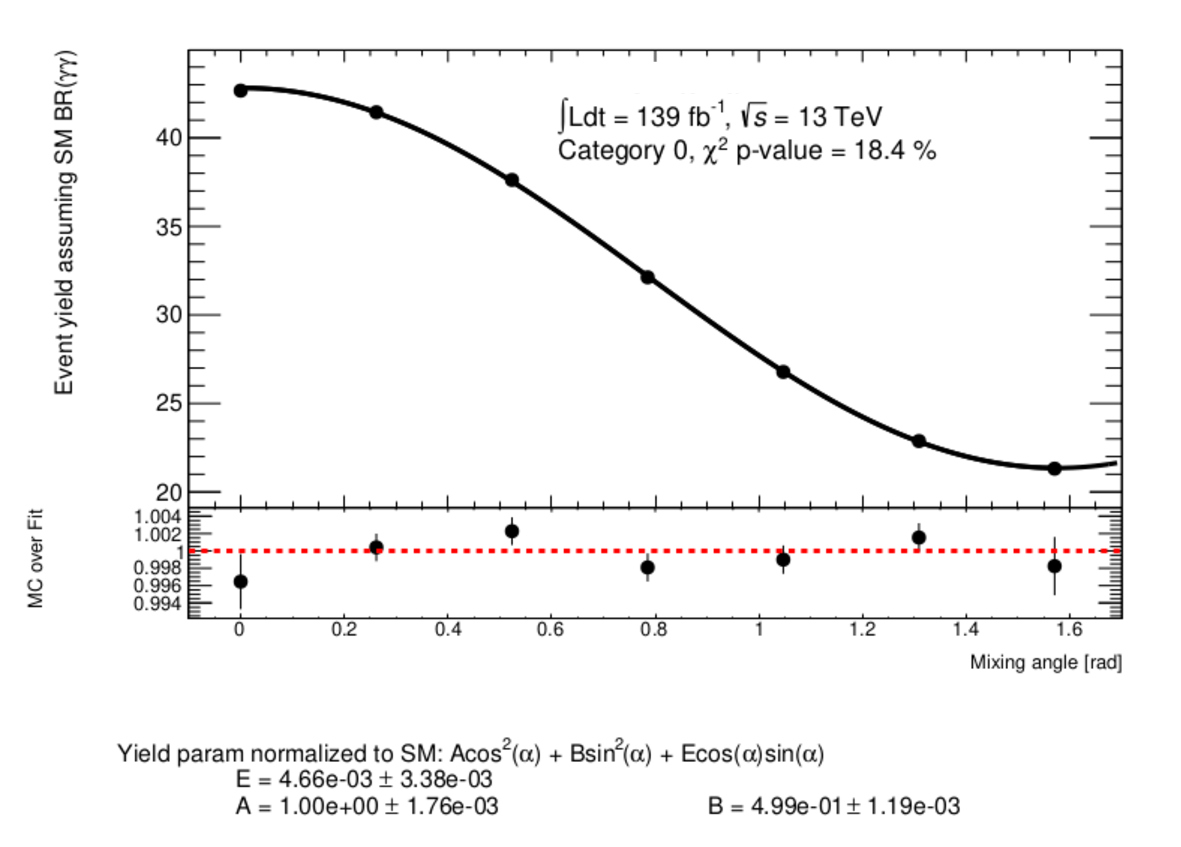
\includegraphics[width=\textwidth]{figures/tthcp_results/yield_ttH_0.pdf}
         \caption{$ttH$}
         \label{fig:ttHYield}
     \end{subfigure}
     \hfill
         \begin{subfigure}[b]{0.3\textwidth}
         \centering
         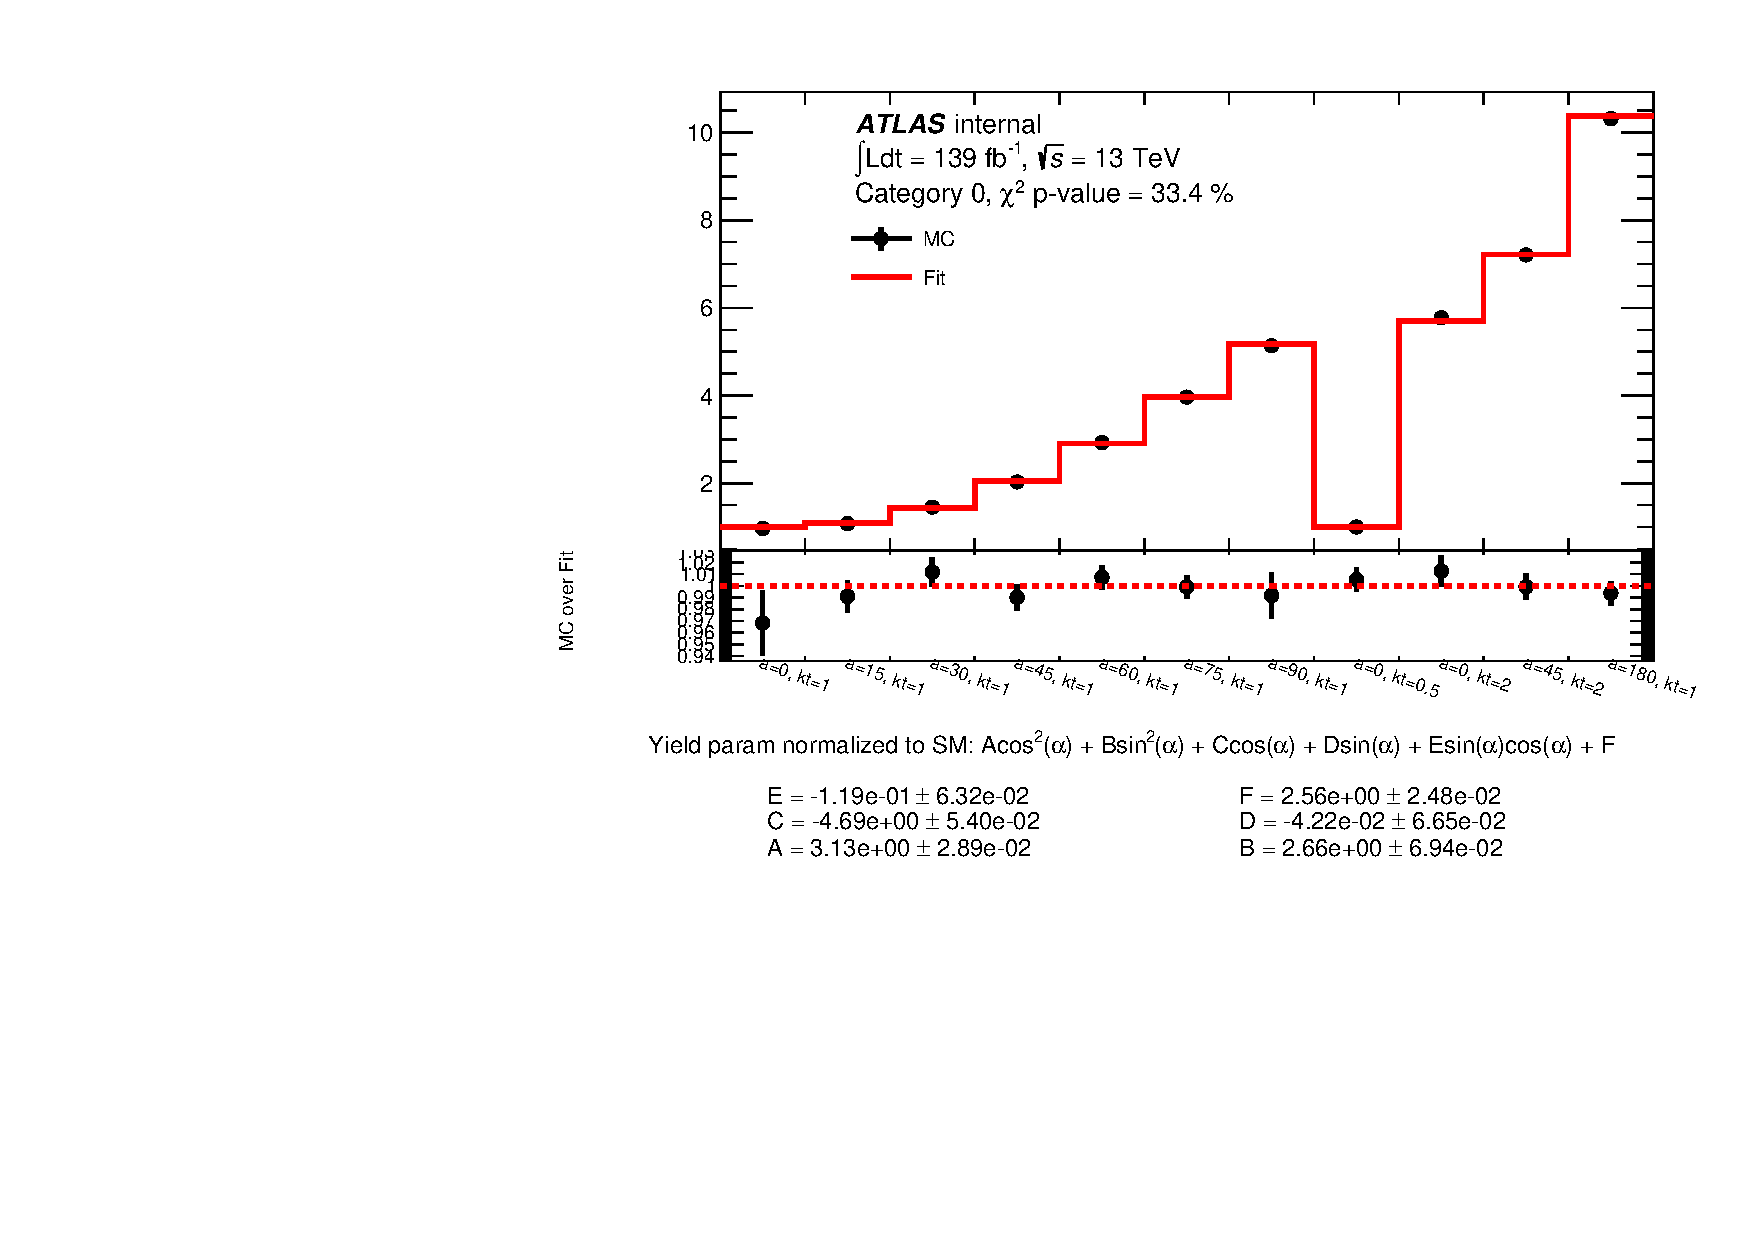
\includegraphics[width=\textwidth]{figures/tthcp_results/yield_tWH_0.pdf}
         \caption{$tWH$}
      \label{fig:tWHYield}
     \end{subfigure}
     \hfill 
        \begin{subfigure}[b]{0.3\textwidth}
         \centering
         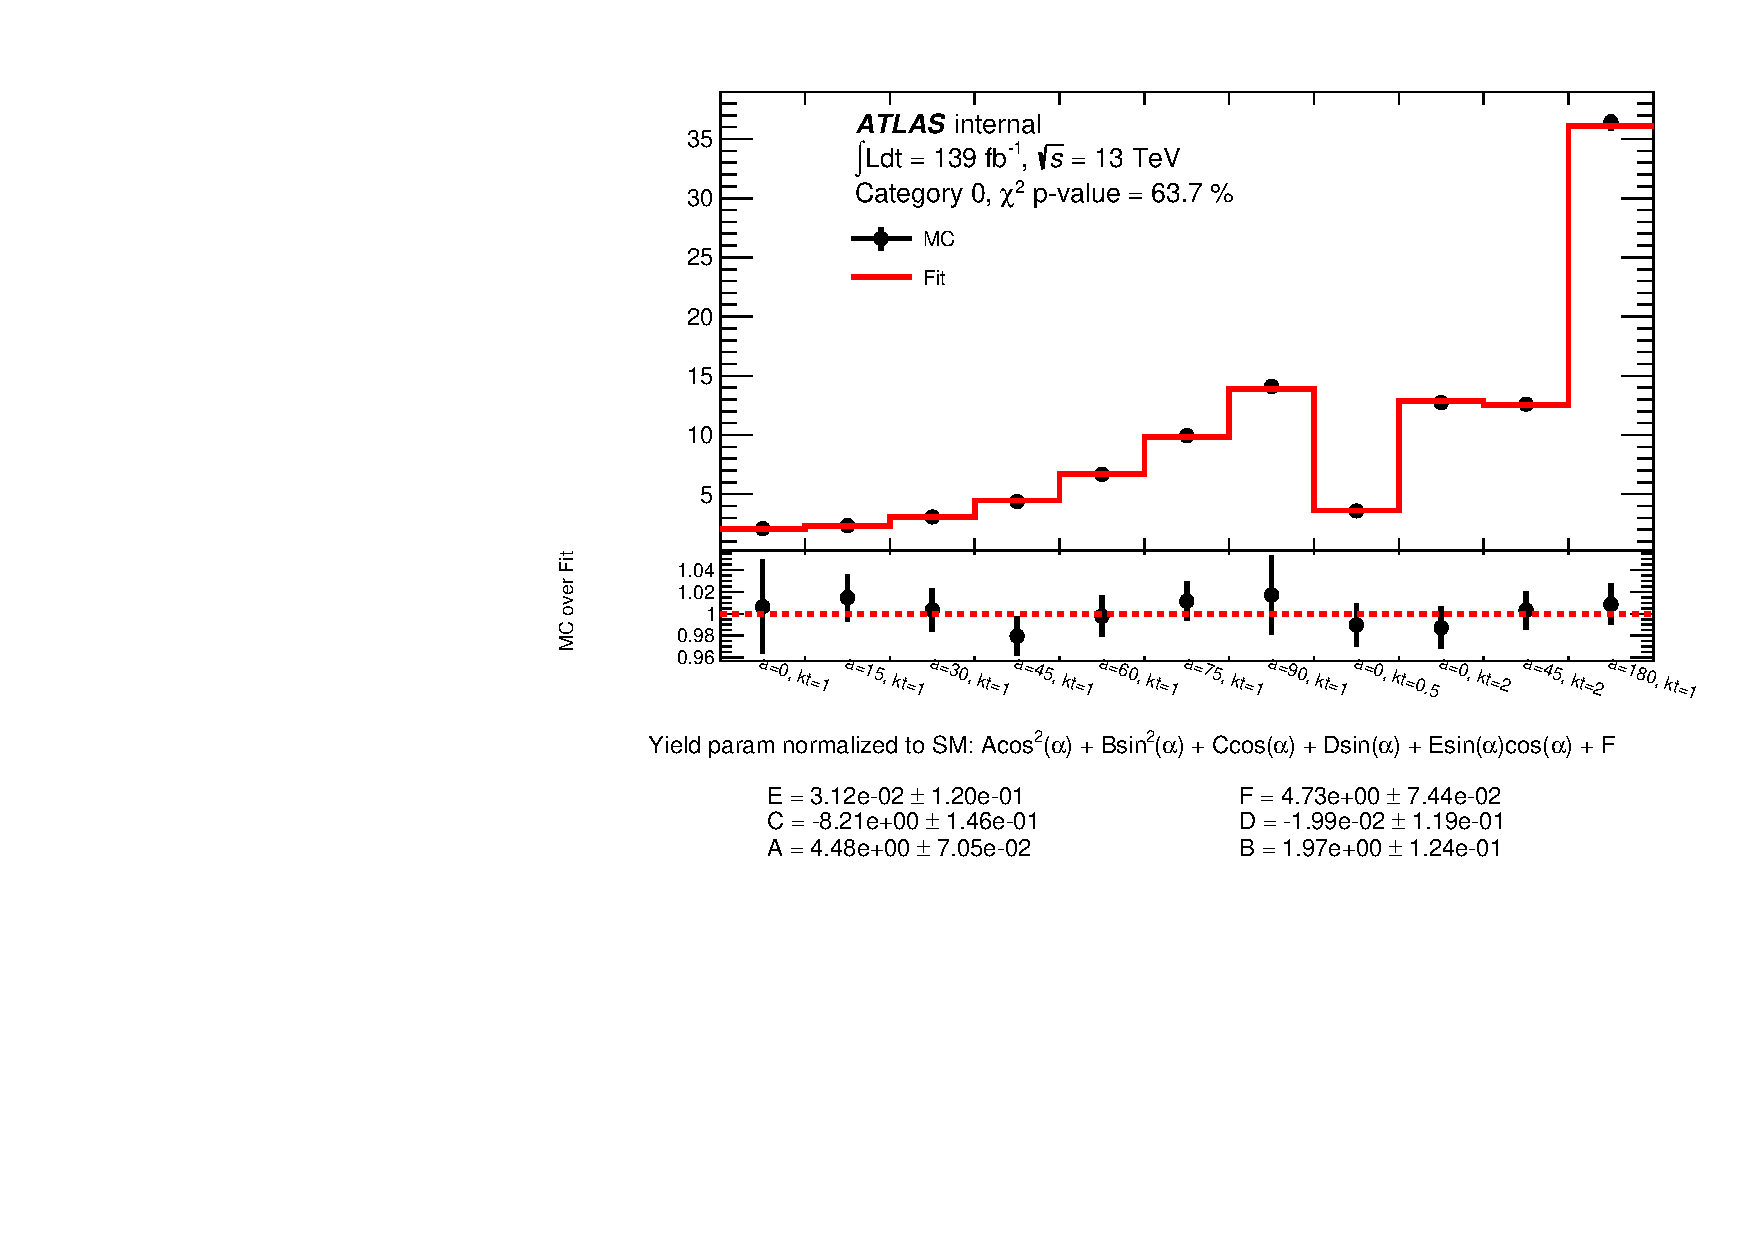
\includegraphics[width=\textwidth]{figures/tthcp_results/yield_tHjb_0.pdf}
         \caption{$tHjb$}
         \label{fig:tHjbYield}
     \end{subfigure}
     \hfill
  \label{fig:YieldParams}
  \caption{Inclusive yield parametrizations as a function of $\kappa_{t}$ and $\alpha$, normalized to $139 fb^{-1}$.}  
\end{figure}


The $ggF$ cross-section and $H \rightarrow \gamma \gamma$ branching ratio can also be parameterized in terms of $\kappa_{t}$ and $\alpha$; this is detailed more in section \ref{sec:results}

\section{Signal and Background Parameterization}

The signal and background shapes are parameterized according to the prescription in Chapter \ref{chap:sigbkgparam}, using a Double-Sided Crystal Ball function for the signal shape and following the spurious signal test procedure for the background parameterization. The DSCB shape does not vary noticeably with $\alpha$, so the Standard-Model Higgs signal DSCB parameterization is used for all $\alpha$ variations occurring in the analysis.

In all categories but one, the $tt\gamma\gamma$ Monte Carlo sample is used for the background template. However, in Hadronic Category 10, a fluctuation in the Monte Carlo causes the spurious signal test to fail- in this category, we choose NTI data as the source of the template due to its lower statistical uncertainty. DSCB parameterizations are given in Tables \ref{tab:sig_param1}-\ref{tab:sig_param2} , while the spurious signal values, template source, choice of functional forms, and fit $\chi^{2}$ probability are shown in Table \ref{tab:spuriousSignal_1}. $Z_{sp}$ denotes the max spurious signal over the statistical uncertainty on the background, while $\mu_{sp}$ denotes the max spurious signal over the expected signal yield in that category.

\begin{table}[!htp]
\begin{center}
\begin{tabular}{lrr}
        \hline
        {} & $\mu_{CB}$ [GeV] & $\sigma_{CB}$ [GeV]  \\
        \hline
        1 & 125.100 & 1.157 \\
        2 & 125.121 & 1.345 \\
        3 & 125.269 & 1.635 \\
        4 & 125.132 & 1.206 \\
        5 & 125.173 & 1.499 \\
        6 & 125.169 & 1.635 \\
        7 & 125.091 & 1.207 \\
        8 & 125.177 & 1.580 \\
        9 & 125.205 & 1.724 \\
        10 & 125.100 & 1.290  \\
        11 & 125.148 & 1.546 \\
        12 & 125.206 & 1.697 \\ \hline

        13 & 125.109 & 1.293 \\
        14 & 125.174 & 1.608 \\
        15 & 125.153 & 1.454 \\
        16 & 125.186 & 1.704 \\
        17 & 125.200 & 1.705 \\
        18 & 125.030 & 1.684 \\
        19 & 125.173 & 1.759 \\
        20 & 125.143 & 1.784 \\
        \hline
\end{tabular}
\caption{Best-fit parameter values for the DSCB Gaussian core in each of the 20 analysis categories.}
\label{tab:sig_param1}
\end{center}
\end{table}

\begin{table}[!htp]
\begin{center}
\begin{tabular}{lrrrr}
        \hline
        {} & $\alpha_{CB}^\text{low}$ & $\alpha_{CB}^{high}$ & $n_{CB}^\text{low}$ & $n_{CB}^{high}$ \\
        \hline
        1 & 1.616 & 1.484 & 6.226 & 15.519 \\
        2 & 1.752 & 1.456 & 4.127 & 15.476 \\
        3 & 1.715 & 1.719 & 4.516 & 11.878 \\
        4 & 1.583 & 1.530 & 4.782 & 5.702 \\
        5 & 1.660 & 1.481 & 6.853 & 15.048 \\
        6 & 1.611 & 1.420 & 8.027 & 35.892 \\
        7 & 1.615 & 1.494 & 5.570 & 11.610 \\
        8 & 1.619 & 1.700 & 5.801 & 7.585 \\
        9 & 1.710 & 1.676 & 4.356 & 12.189 \\
        10 & 1.804 & 1.597 & 13.580 & 7.932 \\
        11 & 1.700 & 1.594 & 4.740 & 7.589 \\
        12 & 1.531 & 1.530 & 8.478 & 13.347\\ \hline
        13 & 1.597& 1.546 & 6.806 & 11.117\\
        14 & 1.659 & 1.549 & 5.237 & 15.030\\
        15 & 1.600 & 1.633 & 5.741 & 5.970\\
        16 & 1.691 & 1.698 & 6.650 & 14.434 \\
        17 & 1.534 & 1.460 & 7.863 & 14.413 \\
        18 & 1.848 & 1.606 & 18.705 & 12.706 \\
        19 & 2.150 & 1.505 & 1.432 & 10.219\\
        20 & 1.553 & 1.578 & 10.752 & 14.703\\
        \hline
\end{tabular}
\caption{Best-fit parameter values for the DSCB exponential tails in each of the 20 analysis categories.}
\label{tab:sig_param2}
\end{center}
\end{table}


\begin{table}[ht]
  \centering
  \begin{tabular}{l l l c c c c c c c c c c c}
    \hline
    Category & Template & Function & $Z_{sp}$ [\%] &  $Z_{sp}^\text{relax}$ [\%] & $\mu_{sp}$ [\%] & $\mu_{sp}^\text{relax}$ [\%] & $N_{sp}$ & Prob($\chi^2$)\\ \hline
1 & $tt+\gamma\gamma$ & Exponential & 28.5 & 0 & 15 & 0 & 0.426 & 90\\
2 & $tt+\gamma\gamma$ & Power Law & -14.2 & 0 & -6.75 & 0 & -0.297 & 82\\
3 & $tt+\gamma\gamma$ & Exponential & 19.6 & 1.83 & 14.9 & 1.43 & 0.26 & 3\\
4 & $tt+\gamma\gamma$ & Exponential & 22.3 & 0 & 35.7 & 0 & 0.311 & 74\\
5 & $tt+\gamma\gamma$ & Power Law & -21.9 & 0 & -32.3 & 0 & -0.566 & 29\\
6 & $tt+\gamma\gamma$ & Exponential & 14.7 & 0 & 18.4 & 0 & 0.335 & 94\\
7 & $tt+\gamma\gamma$ & Exponential & 35.4 & 0 & 90.9 & 0 & 0.644 & 1\\
8 & $tt+\gamma\gamma$ & Exponential & -28.6 & 0 & -47.7 & 0 & -1.23 & 85\\
9 & $tt+\gamma\gamma$ & Power Law & -9.45 & 0 & -12.2 & 0 & -0.264 & 79\\
10 & NTI & Power Law & -89.5 & 0 & -1180 & -8.09 & -1.31 & 62\\
11 & $tt+\gamma\gamma$ & Exponential & 79 & 0 & 324 & 0 & 4.5 & 26\\
12 & $tt+\gamma\gamma$ & Exponential & 28.8 & 0 & 45 & 0 & 3.05 & 48\\ \hline
13 & $tt+\gamma\gamma$ & Exponential & 18 & 0.852 & 5.04 & 0.246 & 0.199 & 48\\
14 & $tt+\gamma\gamma$ & Exponential & 7.17 & 0 & 3.35 & 0 & 0.129 & 46\\
15 & $tt+\gamma\gamma$ & Power Law & -17.1 & 0 & -19.9 & 0 & -0.205 & 39\\
16 & $tt+\gamma\gamma$ & Exponential & 15.5 & 0 & 19.3 & 0 & 0.398 & 66\\
17 & $tt+\gamma\gamma$ & Power Law & -22 & -5.22 & -17.4 & -4.27 & -0.393 & 12\\
18 & $tt+\gamma\gamma$ & Exponential & 43.2 & 1.85 & 319 & 16.5 & 0.761 & 57\\
19 & $tt+\gamma\gamma$ & Power Law & -25.5 & 0 & -117 & 0 & -0.498 & 81\\
20 & $tt+\gamma\gamma$ & Exponential & 5.97 & 0 & -19.8 & 0 & -0.135 & 90\\ \hline
    \hline
  \end{tabular}
  \caption{Spurious signal test results in the 20 analysis categories.}
  \label{tab:spuriousSignal_1}
\end{table}

\section{Systematic Uncertainty}

Uncertainties can effect both the overall yield of a given physics process and the migration of events between categories. For non-top Higgs processes (excluding $ggF$), only the uncertainties on the overall yield are calculated; however, for $ttH$, $tWH$, $tHjb$, and $ggF$, several migration uncertainties are accounted for as well.

\subsection{Theory Systematics}

Theory systematic uncertainties are designed to account for the precision (or imprecision) of the knowledge with which the models used in the analysis are constructed. These take on a number of different forms, including uncertainties on the parton distribution functions (PDFs), uncertainties on the QCD renormalization and factorization scale, and mismodelling of processes containing final-state b-jets.

QCD Renormalization Scale and Factorization Scale uncertainties are both calculated by varying the relevant QCD scale up or down by a factor of two in the Monte Carlo generator, while the PDF and strong coupling constant $\alpha_{s}$ uncertainties are calculated by varying the parameters according to the relevant LHAPDF \cite{LHAPDF} or PDF4LHC \cite{PDF4LHC} prescriptions.

Inclusive parametrization of the QCD and PDF uncertainties on a given process can be used when the effects of category migration are expected to be negligible. The inclusive parameterization of the QCD and PDF uncertainties on non-top Standard Model Higgs processes ($VBF$, $WH$, $ZH$ and $bbH$) is taken from \cite{YellowReport4}. However, previous analyses (\cite{Wb} \cite{Zb} \cite{ttbb} \cite{HZZ4l}) have shown that  processes containing final-state b-jets are poorly-modelled even after applying these yield uncertainties, so we apply a conservative 100\% uncertainty on the yield of $VBF$, $WH$, $ZH$ and $ggF$ in our analysis. This 100\% heavy-flavor uncertainty is not applied to $bbH$ due to its negligible contribution to the overall signal yield in the targeted analysis categories.

Similarly, the underlying event and parton showering uncertainties (UEPS) governed by the choice of MC showering tool are chosen by utilizing the Monte Carlo samples generated with the Herwig7 \cite{Herwig} showering tool rather than the Pythia8 tool \cite{Pythia8.2}. The uncertainty is given by:

\begin{equation}
UEPS= \frac{n_{Herwig}-n_{Pythia}}{n_{Pythia}}
\end{equation}

for each process in each category.

Similarly, a Monte Carlo generator uncertainty is calculated for $ttH$ and $ggH$ by comparing the Madgraph5\_aMC@NLO and Powheg samples.

Finally, an additional nuisance parameter is included to account for the theoretical uncertainty on the $H \rightarrow \gamma \gamma$ branching ratio. The number of nuisance parameters corresponding to each of the theoretical uncertainties and the form of the constraint term for each is given in Table \ref{tab:theorysyst}.

\begin{table}[ht]
\begin{center}
\begin{tabular}{lccccc}
\hline
Source & Number of NPs & Constraint type \\ \hline
$ttH$ QCD scale & 1 & log normal \\
$ttH$ PDF+$\alpha_S$ & 1 & log normal \\
$ttH$ UEPS & 1 & log normal \\
$ttH$ hard-process generator & 1 & log normal \\ \hline
$tHjb$ QCD scale& 1 & log normal \\
$tHjb$ PDF+$\alpha_S$ & 1 & log normal \\
$tHjb$ UEPS & 1 & log normal \\ \hline
$tWH$ QCD scale& 1 & log normal \\
$tWH$ PDF+$\alpha_S$ & 1 & log normal \\
$tWH$ UEPS & 1 & log normal \\ \hline
$ggH$ UEPS & 1 & log normal \\
$ggH$ hard-process generator & 1 & log normal \\
$bbH$ YR4 QCD scale & 1 & asymmetric \\
$bbH$ YR4 PDF + $\alpha_S$ & 1 & asymmetric \\
Non-top Heavy Flavor & 3 ($ggH$, $VBF$, $VH$) & log normal \\
$H\rightarrow\gamma\gamma$ BR & 1 & asymmetric \\
\hline
\end{tabular}
\end{center}
\vspace{-0.5cm}
\caption{A summary of the theory uncertainties used in the likelihood model.}
\label{tab:theorysyst}
\end{table}

\subsection{Experimental Systematics}

Due to the complexity of reconstructing physics objects, a large number of experimental systematics must also be calculated.
These include:

\begin{itemize}
\item Beam luminosity uncertainty \cite{ATLAS-CONF-2019-021}
\item Trigger uncertainty \cite{trigger} \cite{triggerperformance}
\item Pileup reweighting
\item Jet uncertainties: energy scale, energy resolution,  flavor-tagging and flavor composition \cite{jetuncs1} \cite{jetuncs2} \cite{jetuncs3} \cite{jetuncs4}
\item Photon uncertainties: energy scale and resolution (which modify the DSCB parameters as per Chapter \ref{chap:sigbkgparam}), photon ID, photon isolation \cite{CERN-EP-2019-145} \cite{photuncs}
\item Electron/muon uncertainties: energy scale, energy resolution, electron/muon ID, electron/muon isolation \cite{CERN-EP-2019-145} \cite{photuncs} \cite{elID-CERN-EP-2018-273} \cite{CERN-EP-2016-033}
\item $E_T^{miss}$ uncertainties: \cite{MET1} \cite{MET2}
\item Higgs mass: \cite{Higgsmass}
\item Background modelling uncertainty: Calculated from spurious signal procedure discussed in Chapter \ref{chap:sigbkgparam}
\end{itemize}

Due to the number of experimental uncertainties considered, a merging scheme is adopted for photon energy scale and resolution systematics to take advantage of similar energy scale and resolution in certain regions of the detector.

The list of theoretical uncertainties and the form of the constraint term for each is given in Table \ref{tab:expsyst}.

\begin{table}[ht]
\begin{center}
\begin{tabular}{lccccc}
\hline
Source & Number of NPs & Constraint type \\ \hline
Yield \\ \hline
Luminosity & 1 & log normal  \\
Photon efficiency & 3 (ID, isolation, trigger) & asymmetric \\
\hline
Yield and Migration \\ \hline
Flavor tagging & 12 & asymmetric \\
Jets & 25 & asymmetric \\
Jet flavor composition and response & 14 & asymmetric \\
Electrons & 2 & asymmetric \\
Muons & 7 & asymmetric\\
Missing $E_{T}$ & 3 & asymmetric\\
Pileup & 1 & asymmetric \\
\hline
Shape \\ \hline
Photon energy scale & 40 (merged scheme) & Gaussian  \\
Photon energy resolution & 5 (merged scheme) & log normal \\
Spurious signal & 20 (1 per category) & Gaussian \\
Measured $m_H$ & 1 & Gaussian \\
\end{tabular}
\end{center}
\vspace{-0.5cm}
\caption{A summary of the experimental uncertainties used in the likelihood model.}
\label{tab:expsyst}
\end{table}

\begin{table}[ht]
\begin{center}
\begin{tabular}{lllll}
Category & QCD (up) & QCD (down) & PDF (up) & PDF (down) \\ \hline
1  &     0.060 &      -0.094 &   0.020 &    -0.020 \\
2  &     0.055 &      -0.089 &   0.016 &    -0.016 \\
3  &     0.028 &      -0.074 &   0.015 &    -0.015 \\
4  &     0.077 &      -0.103 &   0.022 &    -0.022 \\
5  &     0.061 &      -0.092 &   0.017 &    -0.017 \\
6  &     0.058 &      -0.089 &   0.014 &    -0.014 \\
7  &     0.091 &      -0.109 &   0.020 &    -0.020 \\
8  &     0.062 &      -0.092 &   0.016 &    -0.016 \\
9  &     0.062 &      -0.091 &   0.015 &    -0.015 \\
10 &     0.095 &      -0.109 &   0.024 &    -0.024 \\
11 &     0.073 &      -0.099 &   0.019 &    -0.019 \\
12 &     0.060 &      -0.090 &   0.015 &    -0.015 \\ \hline
13 &     0.068 &      -0.097 &   0.017 &    -0.017 \\
14 &     0.067 &      -0.094 &   0.015 &    -0.015 \\
15 &     0.066 &      -0.095 &   0.017 &    -0.017 \\
16 &     0.045 &      -0.082 &   0.014 &    -0.014 \\
17 &     0.048 &      -0.079 &   0.013 &    -0.013 \\
18 &     0.061 &      -0.089 &   0.014 &    -0.014 \\
19 &     0.047 &      -0.081 &   0.013 &    -0.013 \\
20 &     0.040 &      -0.071 &   0.014 &    -0.014 \\ \hline
\hline
\end{tabular}
\end{center}
\vspace{-0.5cm}
\caption{Relative QCD renormalization and factorization scale ($\mu_R$, $\mu_F$) and PDF uncertainties on the Standard Model $ttH$ sample.}
\label{tab:qcdpdf_ttH}
\end{table}

 \begin{table}[ht]
 \begin{center}
 \begin{tabular}{lllll}
 Category & QCD (up) & QCD (down) & PDF (up) & PDF (down) \\ \hline
1  &     0.026 &      -0.048 &   0.028 &    -0.028 \\
2  &     0.092 &      -0.155 &   0.029 &    -0.029 \\
3  &     0.264 &      -0.397 &   0.026 &    -0.026 \\
4  &     0.017 &      -0.025 &   0.028 &    -0.028 \\
5  &     0.052 &      -0.091 &   0.023 &    -0.023 \\
6  &     0.125 &      -0.197 &   0.020 &    -0.020 \\
7  &     0.021 &      -0.027 &   0.030 &    -0.030 \\
8  &     0.048 &      -0.074 &   0.025 &    -0.025 \\
9  &     0.090 &      -0.140 &   0.024 &    -0.024 \\
10 &     0.047 &      -0.046 &   0.033 &    -0.033 \\
11 &     0.021 &      -0.026 &   0.029 &    -0.029 \\
12 &     0.038 &      -0.045 &   0.022 &    -0.022 \\ \hline
13 &     0.036 &      -0.046 &   0.027 &    -0.027 \\
14 &     0.139 &      -0.219 &   0.021 &    -0.021 \\
15 &     0.018 &      -0.026 &   0.028 &    -0.028 \\
16 &     0.045 &      -0.038 &   0.020 &    -0.020 \\
17 &     0.028 &      -0.037 &   0.021 &    -0.021 \\
18 &     0.037 &      -0.037 &   0.029 &    -0.029 \\
19 &     0.012 &      -0.010 &   0.022 &    -0.022 \\
20 &     0.048 &      -0.070 &   0.021 &    -0.021 \\ \hline
 \hline
 \end{tabular}
 \end{center}
 \vspace{-0.5cm}
 \caption{Relative QCD renormalization and factorization scale ($\mu_R$, $\mu_F$) and PDF uncertainties on the Standard Model $tWH$ Madgraph sample.}
 \label{tab:qcdpdf_tWH}
 \end{table}



 \begin{table}[ht]
 \begin{center}
 \begin{tabular}{lllll}
 Category & QCD (up) & QCD (down) & PDF (up) & PDF (down) \\ \hline
1  &     0.070 &      -0.077 &   0.023 &    -0.023 \\
2  &     0.036 &      -0.044 &   0.026 &    -0.026 \\
3  &     0.131 &      -0.108 &   0.013 &    -0.013 \\
4  &     0.116 &      -0.105 &   0.013 &    -0.013 \\
5  &     0.083 &      -0.081 &   0.039 &    -0.039 \\
6  &     0.012 &      -0.026 &   0.024 &    -0.024 \\
7  &     0.068 &      -0.075 &   0.025 &    -0.025 \\
8  &     0.044 &      -0.057 &   0.070 &    -0.070 \\
9  &     0.035 &      -0.042 &   0.050 &    -0.050 \\
10 &     0.070 &      -0.078 &   0.055 &    -0.055 \\
11 &     0.071 &      -0.077 &   0.013 &    -0.013 \\
12 &     0.028 &      -0.047 &   0.010 &    -0.010 \\ \hline
13 &     0.028 &      -0.051 &   0.022 &    -0.022 \\
14 &     0.006 &      -0.021 &   0.015 &    -0.015 \\
15 &     0.097 &      -0.094 &   0.021 &    -0.021 \\
16 &     0.052 &      -0.062 &   0.018 &    -0.018 \\
17 &     0.054 &      -0.057 &   0.015 &    -0.015 \\
18 &     0.072 &      -0.079 &   0.016 &    -0.016 \\
19 &     0.077 &      -0.080 &   0.013 &    -0.013 \\
20 &     0.023 &      -0.037 &   0.035 &    -0.035 \\ \hline
 \hline
 \end{tabular}
 \end{center}
 \vspace{-0.5cm}
 \caption{Relative QCD renormalization and factorization scale ($\mu_R$, $\mu_F$) and PDF uncertainties on the Standard Model $tHjb$ Madgraph sample.}
 \label{tab:qcdpdf_tHjb}
 \end{table}

\begin{table}[ht]
\begin{center}
\begin{tabular}{lllll}
Category & $ttH$ & $tHjb$ & $tWH$ & $ggF$ \\ \hline
1  &       -0.063 &         0.091 &        0.106 &    -0.067 \\
2  &       -0.014 &        -0.195 &       -0.133 &     0.537 \\
3  &        0.074 &         0.000 &       -0.074 &    -0.502 \\
4  &       -0.054 &        -0.407 &       -0.361 &     0.307 \\
5  &       -0.006 &        -0.452 &       -0.150 &     0.273 \\
6  &        0.061 &        -0.241 &       -0.358 &    -0.967 \\
7  &       -0.088 &        -0.215 &       -0.143 &    -0.015 \\
8  &        0.008 &        -0.123 &       -0.028 &     1.035 \\
9  &        0.060 &         0.479 &       -0.054 &     0.207 \\
10 &       -0.027 &         0.441 &       -0.267 &     0.292 \\
11 &       -0.050 &        -0.120 &        0.081 &     0.292 \\
12 &        0.001 &        -0.111 &        0.026 &     0.588 \\ \hline
13 &       -0.046 &        -0.350 &       -0.082 &     0.096 \\
14 &        0.046 &        -0.373 &        0.024 &     0.586 \\
15 &       -0.109 &        -0.141 &       -0.065 &     0.071 \\
16 &       -0.010 &        -0.192 &       -0.239 &     0.000 \\
17 &       -0.022 &         0.354 &        0.157 &    -1.000 \\
18 &       -0.091 &         0.215 &       -0.184 &     1.117 \\
19 &       -0.079 &         0.277 &       -0.131 &    -0.736 \\
20 &       -0.025 &        -0.240 &        0.253 &    -0.125 \\ \hline
\hline
\end{tabular}
\end{center}
\vspace{-0.5cm}
\caption{Relative effect [(Varied-Nominal)/Nominal] of the underlying event and parton showering (UEPS) theoretical uncertainties for $ttH$, $tHjb$, $tWH$ and $ggF$.}
\label{tab:ueps}
\end{table}

\begin{table}[ht]
\begin{center}
\begin{tabular}{llll}
Category & $ggF$ & $ttH$ \\ \hline
\hline
1  &     -0.870 &      0.014 \\
2  &     -0.515 &     -0.043 \\
3  &      0.000 &     -0.097 \\
4  &     -0.160 &      0.025 \\
5  &      0.281 &     -0.056 \\
6  &     -0.772 &     -0.072 \\
7  &     -0.124 &      0.053 \\
8  &      0.004 &     -0.057 \\
9  &      0.070 &     -0.078 \\
10 &     -0.382 &     -0.018 \\
11 &     -0.188 &      0.022 \\
12 &      0.190 &     -0.031 \\ \hline
13 &     -0.969 &      0.035 \\
14 &      0.000 &     -0.026 \\
15 &     -0.356 &      0.088 \\
16 &      0.000 &      0.005 \\
17 &      0.000 &      0.009 \\
18 &     -2.032 &      0.075 \\
19 &      0.943 &      0.056 \\
20 &     -0.866 &      0.034 \\ \hline
\end{tabular}
\end{center}
\vspace{-0.5cm}
\caption{Generator uncertainties on $ggF$ (aMCnloPy8 $ggF$ - PowhegPy8 $ggF$)/(PowhegPy8 $ggF$) and $ttH$ (PowhegPy8 $ttH$ - aMCnloPy8 $ttH$)/(aMCnloPy8 $ttH$) in each analysis category. }
\label{tab:mcgen}
\end{table}

\section{Results and Interpretations}\label{sec:results}

The fitted diphoton mass spectrum in each category and inclusively (weighted by $ln(1+S/B)$ to visually enhance the contributions of signal-enriched categories) is shown in Figures \ref{fig:invmass_had1}-\ref{fig:invmass_tot}. We observe that the Higgs signal peak is strongest in the more CP-even sensitive categories (3, 6, 9, 12, 14, 17, and 20), rather than the more CP-odd sensitive ones (1, 4, 7, 10, 13, 16, and 19), thus lending credence to the Standard Model prediction. Numerically, we can extract a number of key metrics:

\begin{itemize}
\item Observed and expected $ttH$ significance
\item Observed and expected upper limits on $tH$ significance
\item 2D limits on the ($\kappa_{t} cos(\alpha)$, $\kappa_{t} sin(\alpha)$) plane
\item 1D limits on $\alpha$, setting $\kappa_{t} = 1$
\end{itemize}

Two potential interpretations of the final two metrics are given in order to properly treat the dependence of $ggF$ and $H \rightarrow \gamma \gamma$ on $\alpha$.

In the first interpretation, existing measurements of $\kappa_{g}$ and $\kappa_{\gamma}$ \cite{couplings80fb} can be used to constrain the $ggF$ and $H \rightarrow \gamma \gamma$ terms. 

In the second, $\kappa_{g}$ and $\kappa_{\gamma}$ are parameterized as in \cite{Ellis} in order to allow them to vary in the fit:

\begin{align}
\begin{aligned}
\kappa_{g}^{2} = 1.11\kappa_{t}^{2}cos(\alpha)^{2} + 2.6\kappa_{t}^{2}sin(\alpha)^{2} - 0.11\kappa_{t}cos(\alpha) \\
\kappa_{\gamma}^{2} = 0.08\kappa_{t}^{2}cos(\alpha)^{2} + 0.18\kappa_{t}^{2}sin(\alpha)^{2} - 0.72\kappa_{t}cos(\alpha) + 1.64
\end{aligned}
\end{align}

The total yields are observed in Figure \ref{fig:yields} and Table \ref{tab:yields}.  

\begin{figure}[htbp]
  \centering
  \subfloat[Category 1: $m_{\gamma\gamma}$ (GeV)]{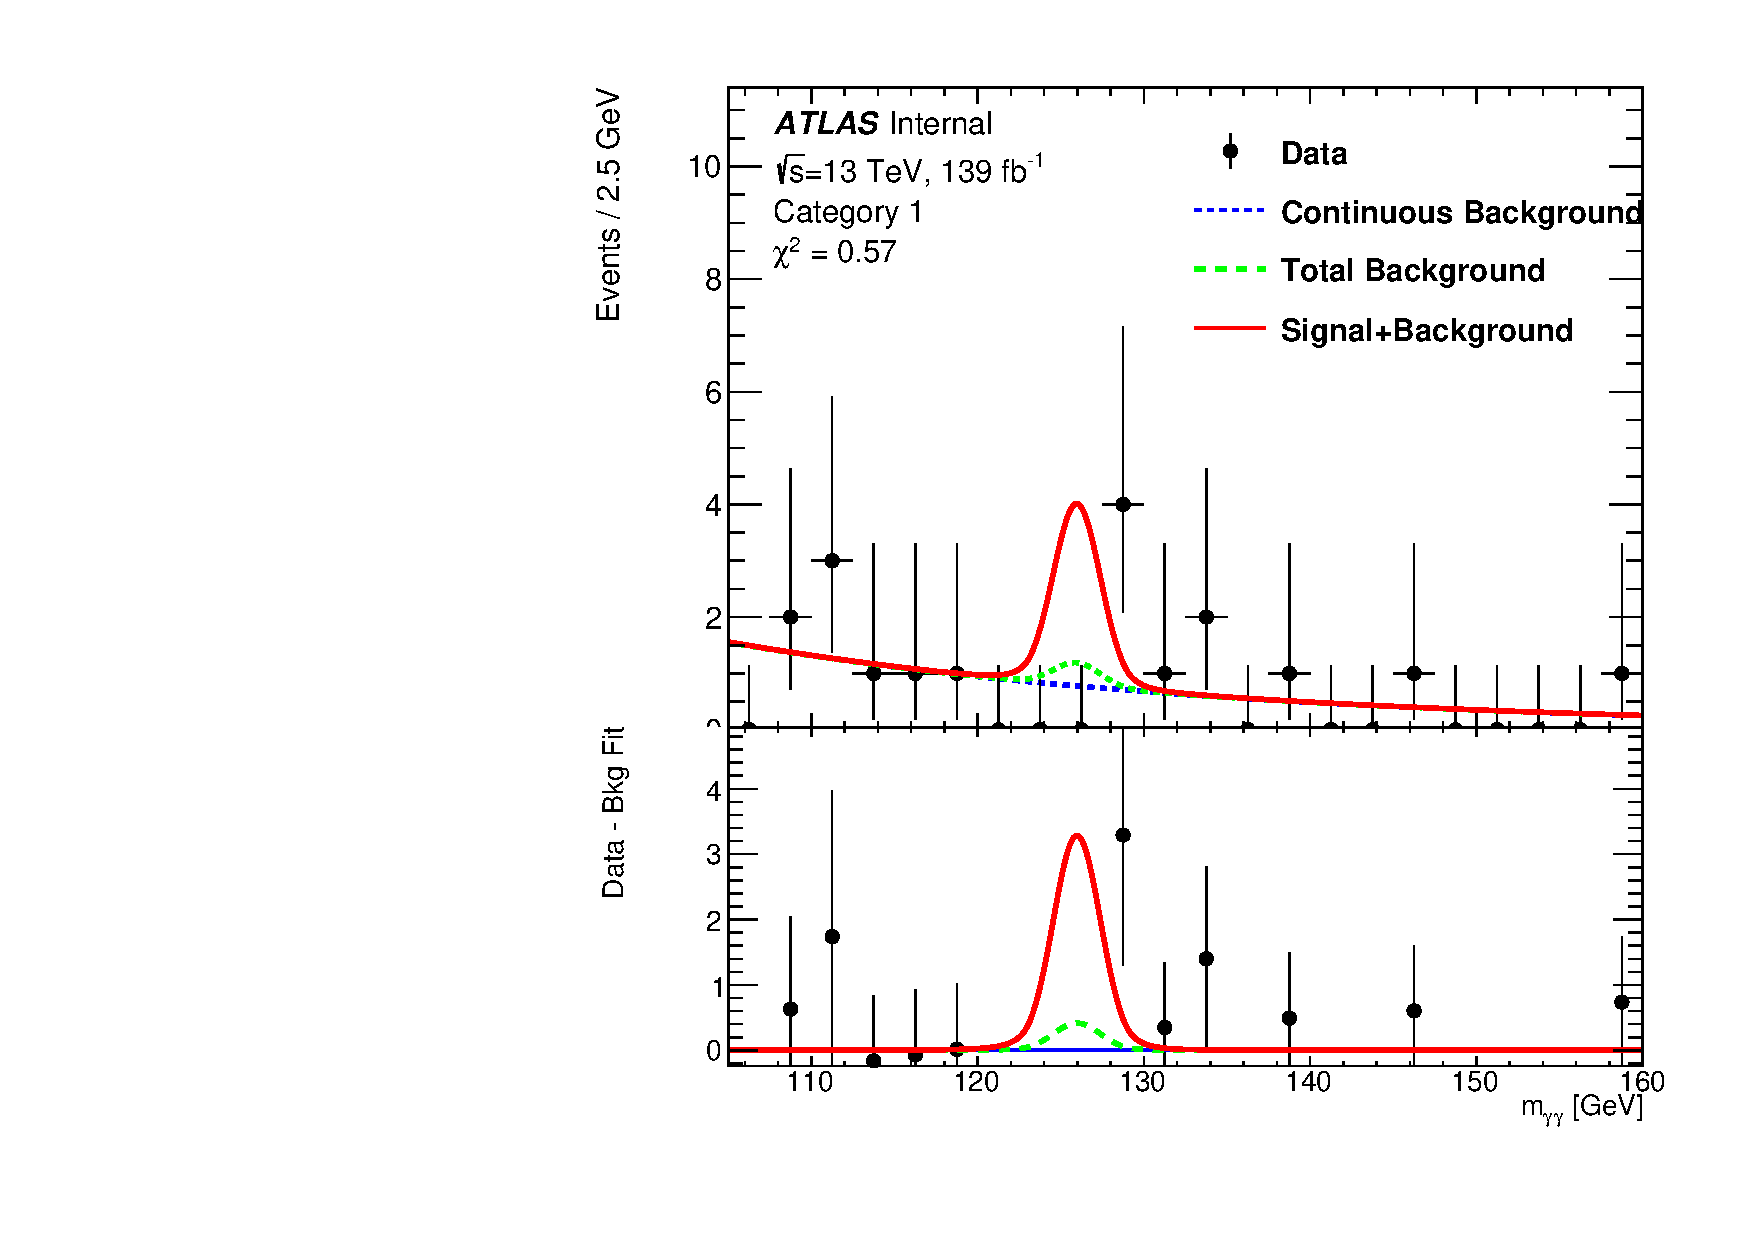
\includegraphics[width=0.3\textwidth]{figures/tthcp_results/Had_1_1.pdf}}
  \subfloat[Category 2: $m_{\gamma\gamma}$ (GeV)]{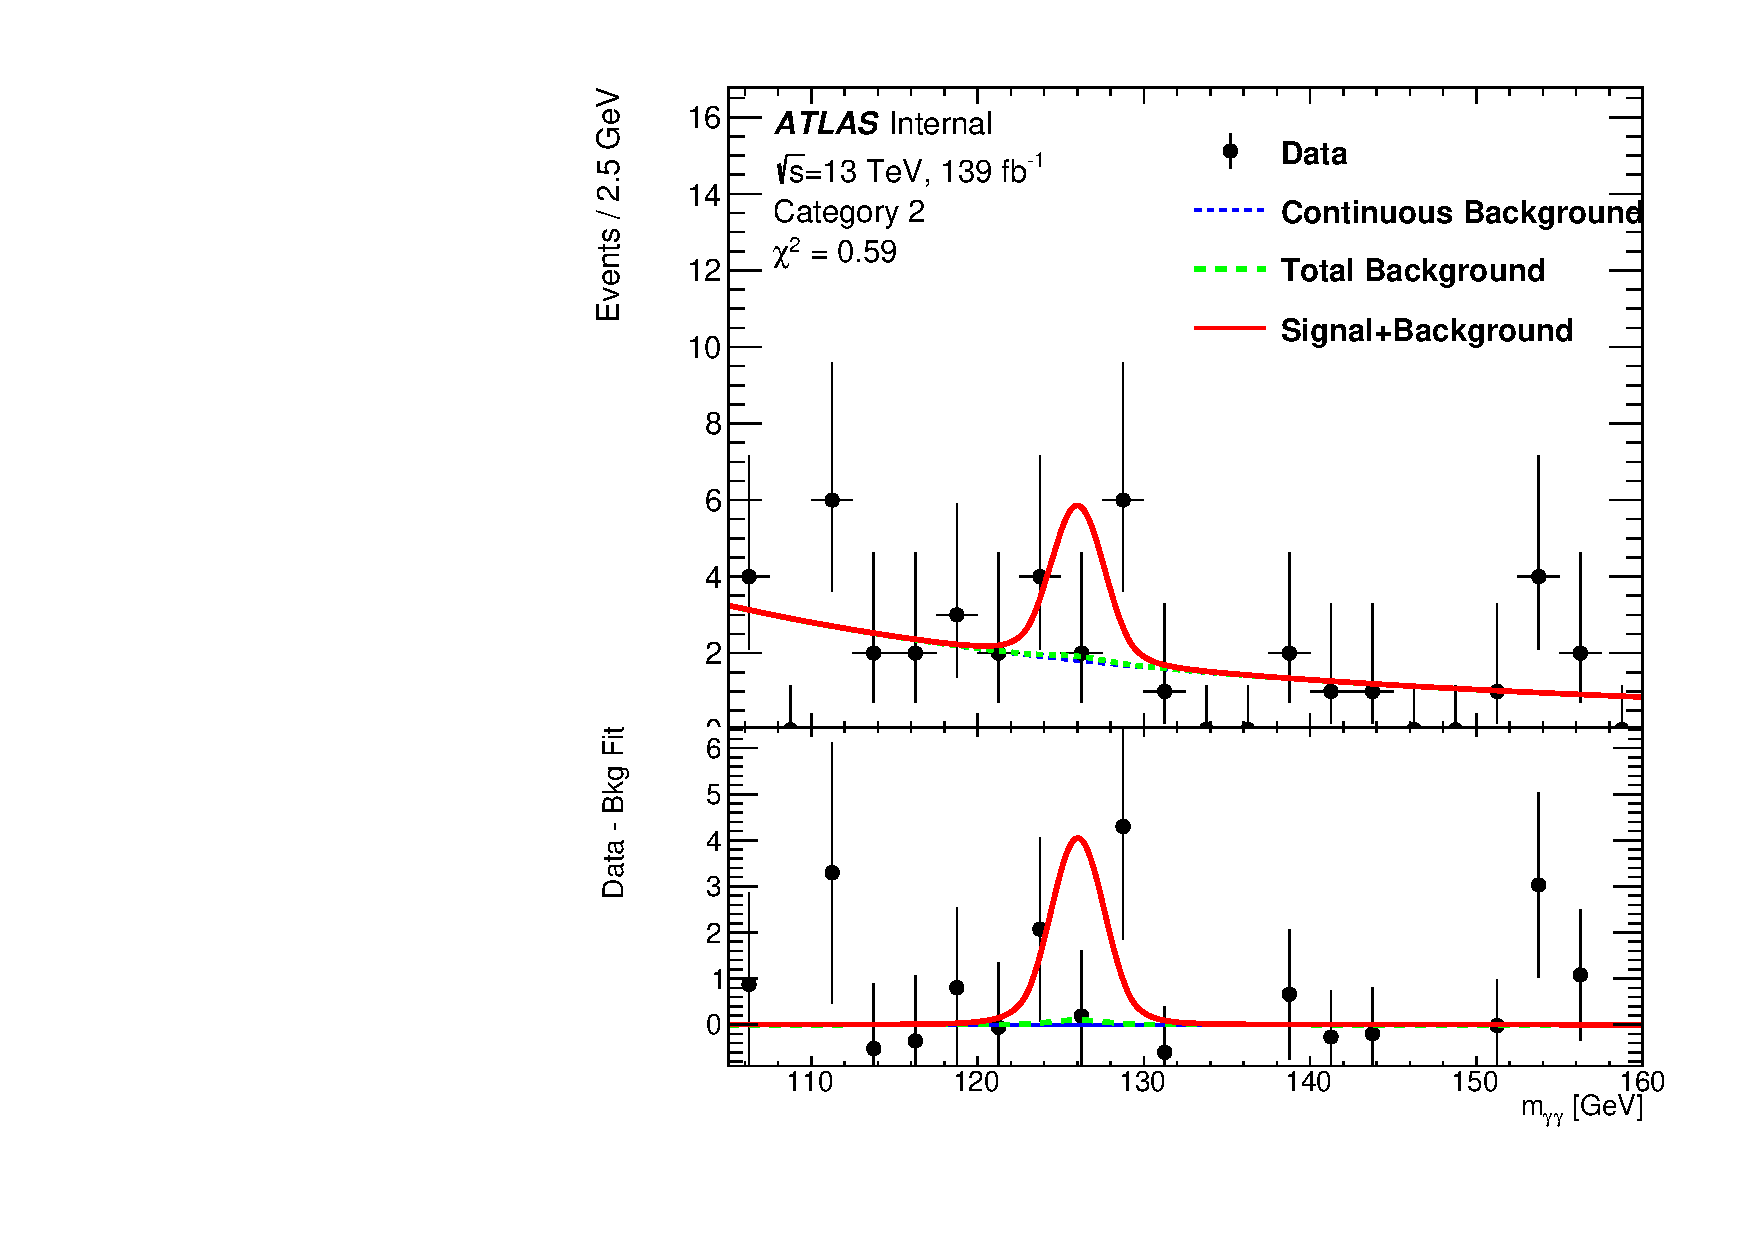
\includegraphics[width=0.3\textwidth]{figures/tthcp_results/Had_1_2.pdf}}
  \subfloat[Category 3: $m_{\gamma\gamma}$ (GeV)]{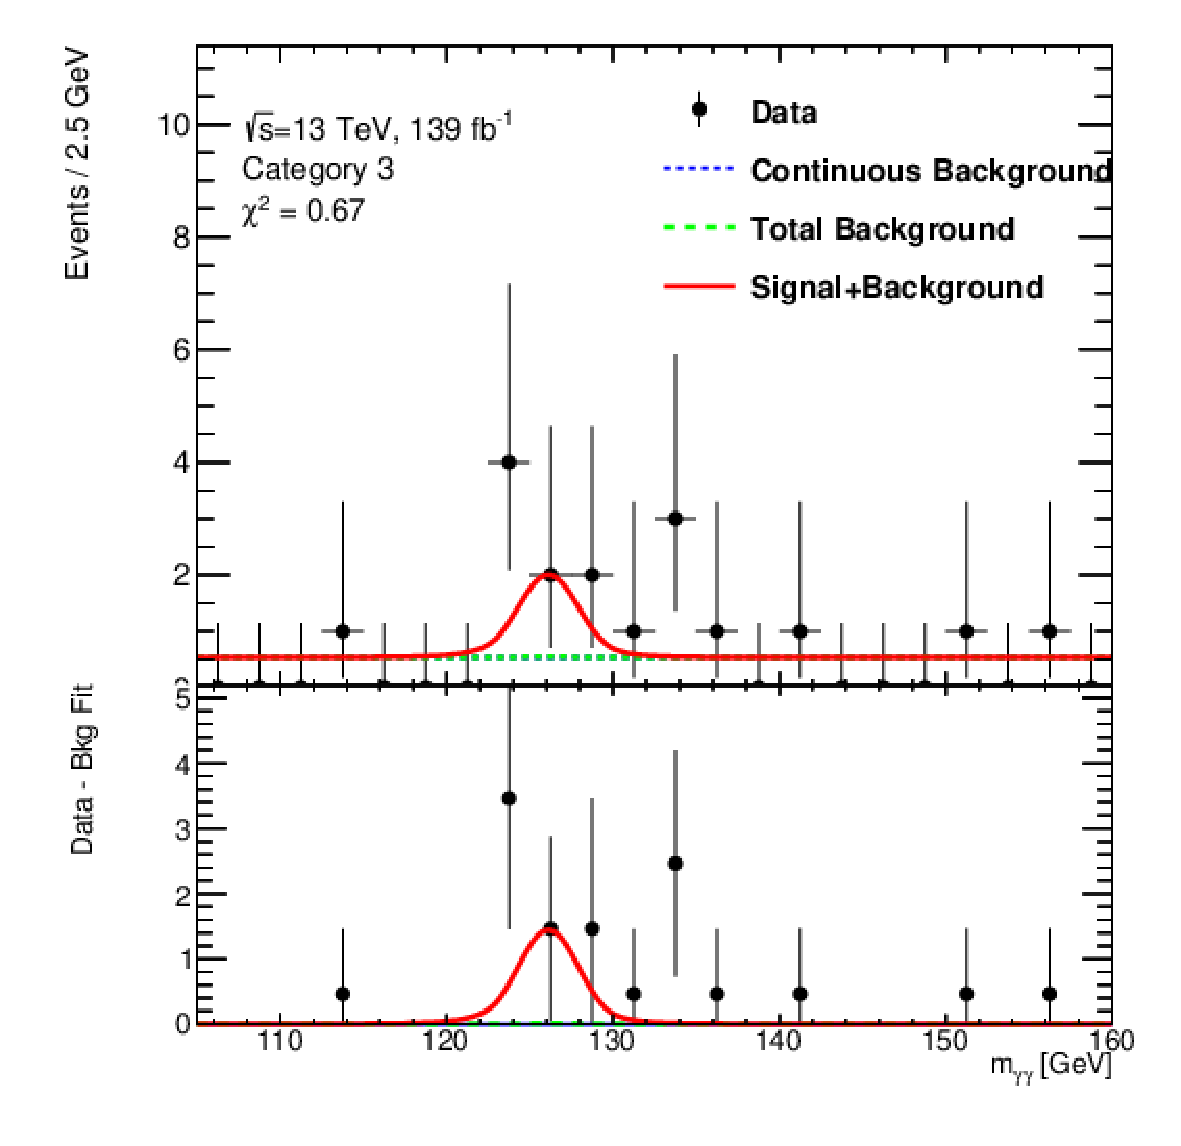
\includegraphics[width=0.3\textwidth]{figures/tthcp_results/Had_1_3.pdf}}\\
  \subfloat[Category 4: $m_{\gamma\gamma}$ (GeV)]{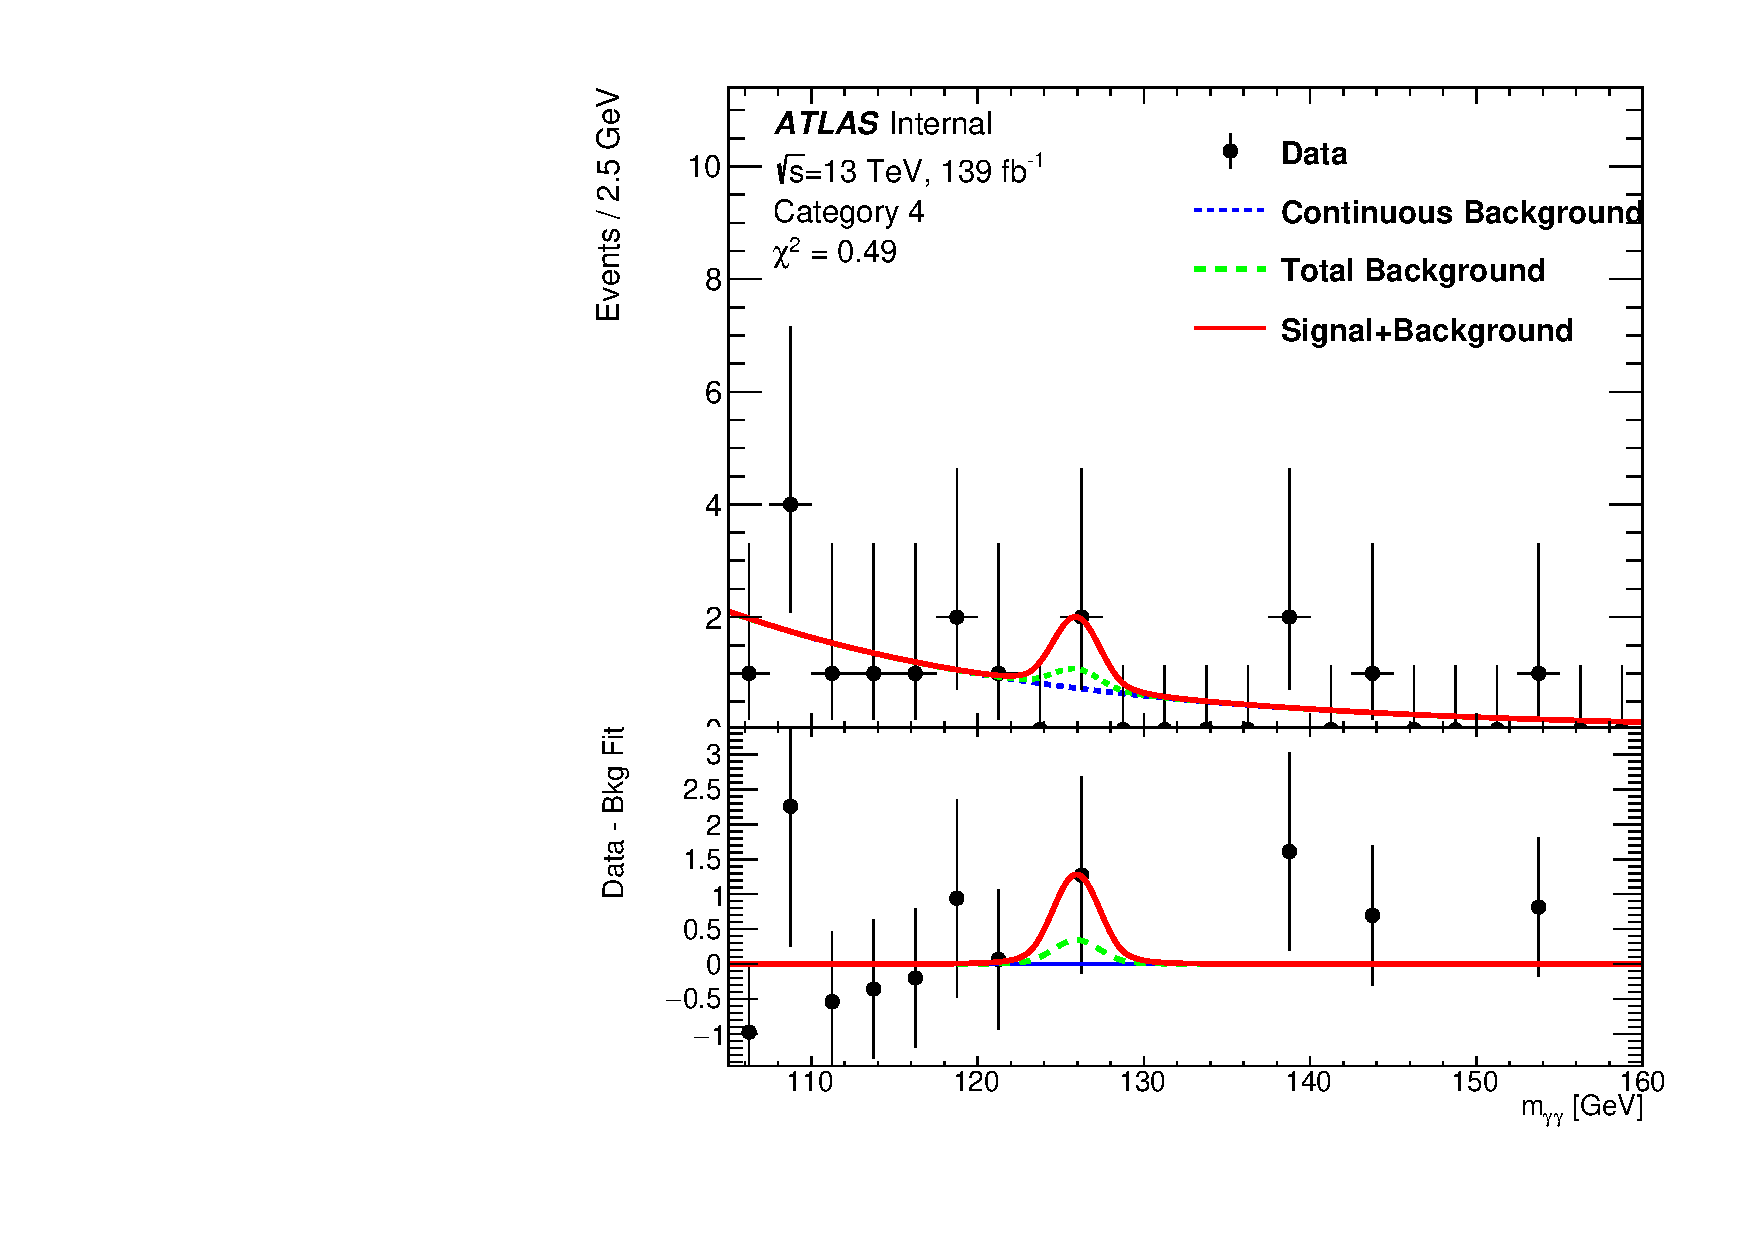
\includegraphics[width=0.3\textwidth]{figures/tthcp_results/Had_2_1.pdf}}
  \subfloat[Category 5: $m_{\gamma\gamma}$ (GeV)]{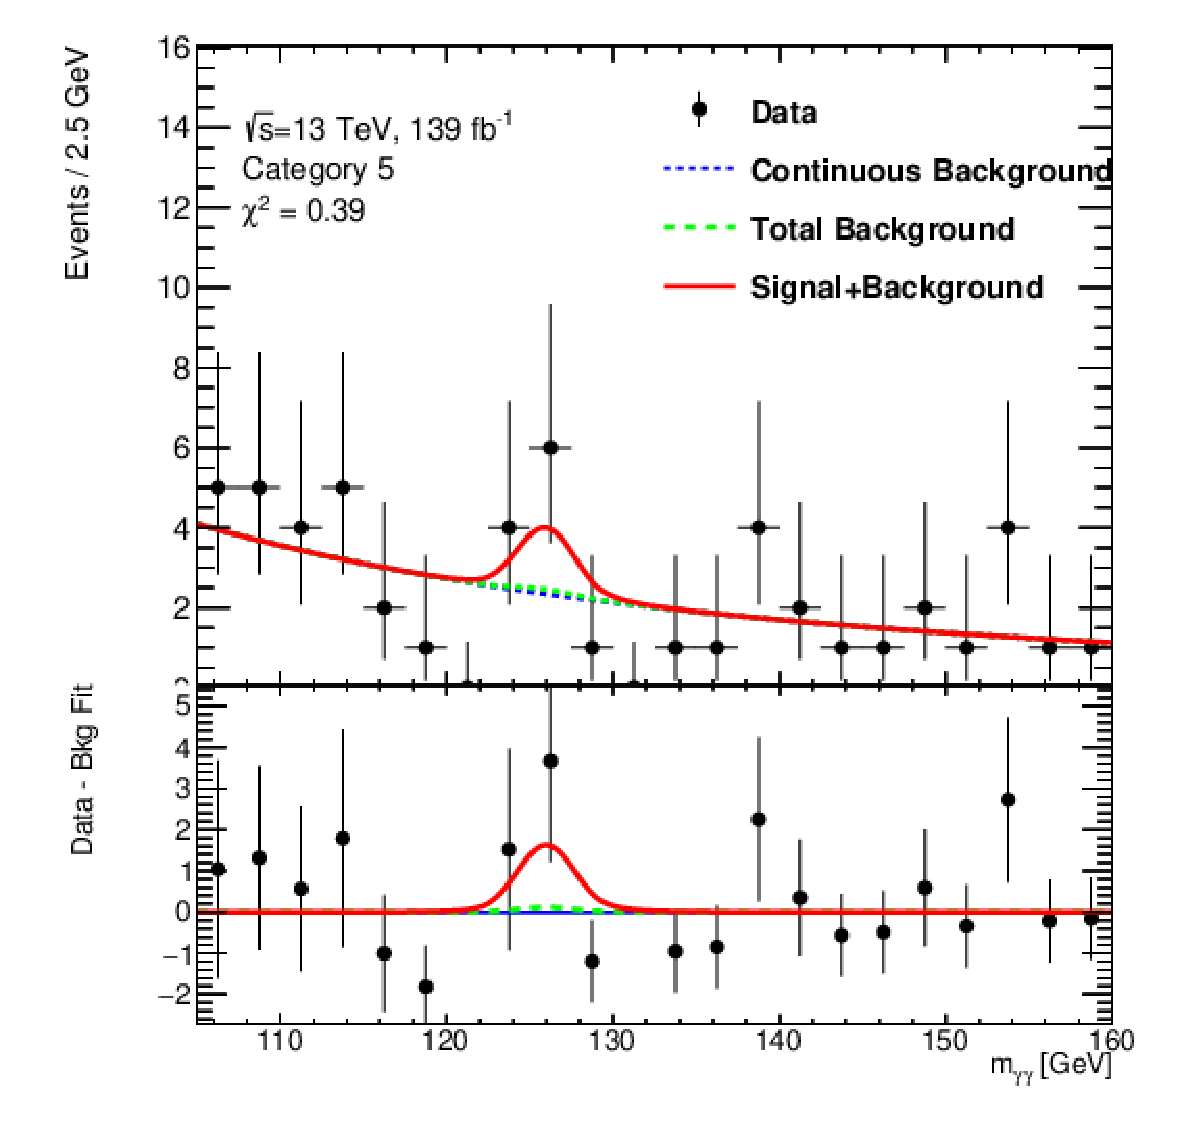
\includegraphics[width=0.3\textwidth]{figures/tthcp_results/Had_2_2.pdf}}
  \subfloat[Category 6: $m_{\gamma\gamma}$ (GeV)]{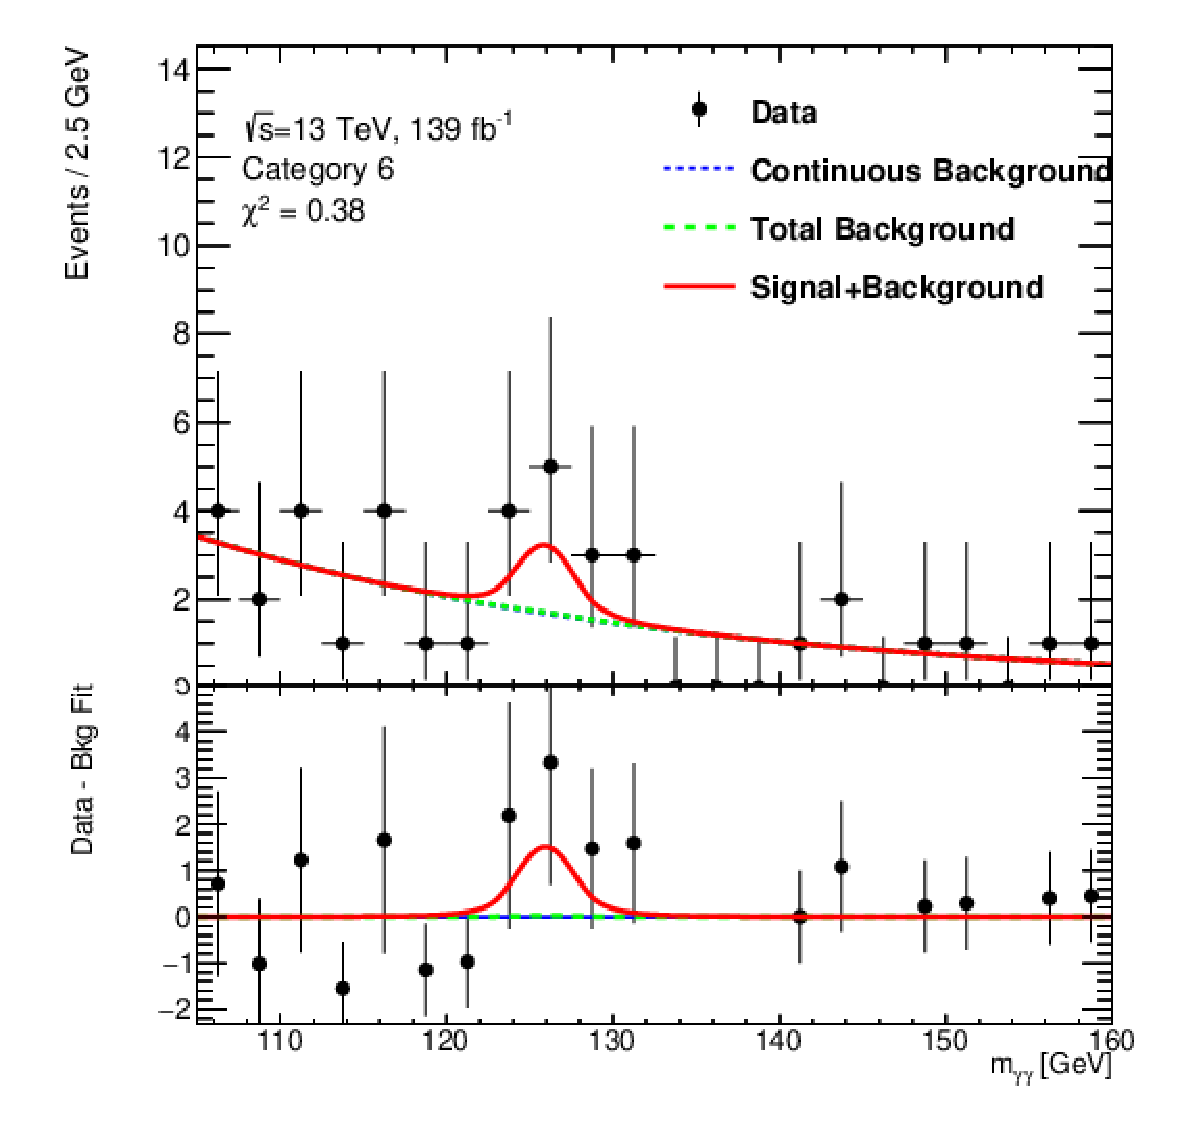
\includegraphics[width=0.3\textwidth]{figures/tthcp_results/Had_2_3.pdf}}
  \caption{Diphoton invariant mass spectrum ($m_{\gamma\gamma}$) in the first six hadronic categories. The fitted continuum background is shown in blue the, total background including non-top Higgs processes is shown in green, and total fitted signal plus background is shown in red.}
    \label{fig:invmass_had1}
\end{figure}

\begin{figure}[htbp]
  \centering
  \subfloat[Category 7: $m_{\gamma\gamma}$ (GeV)]{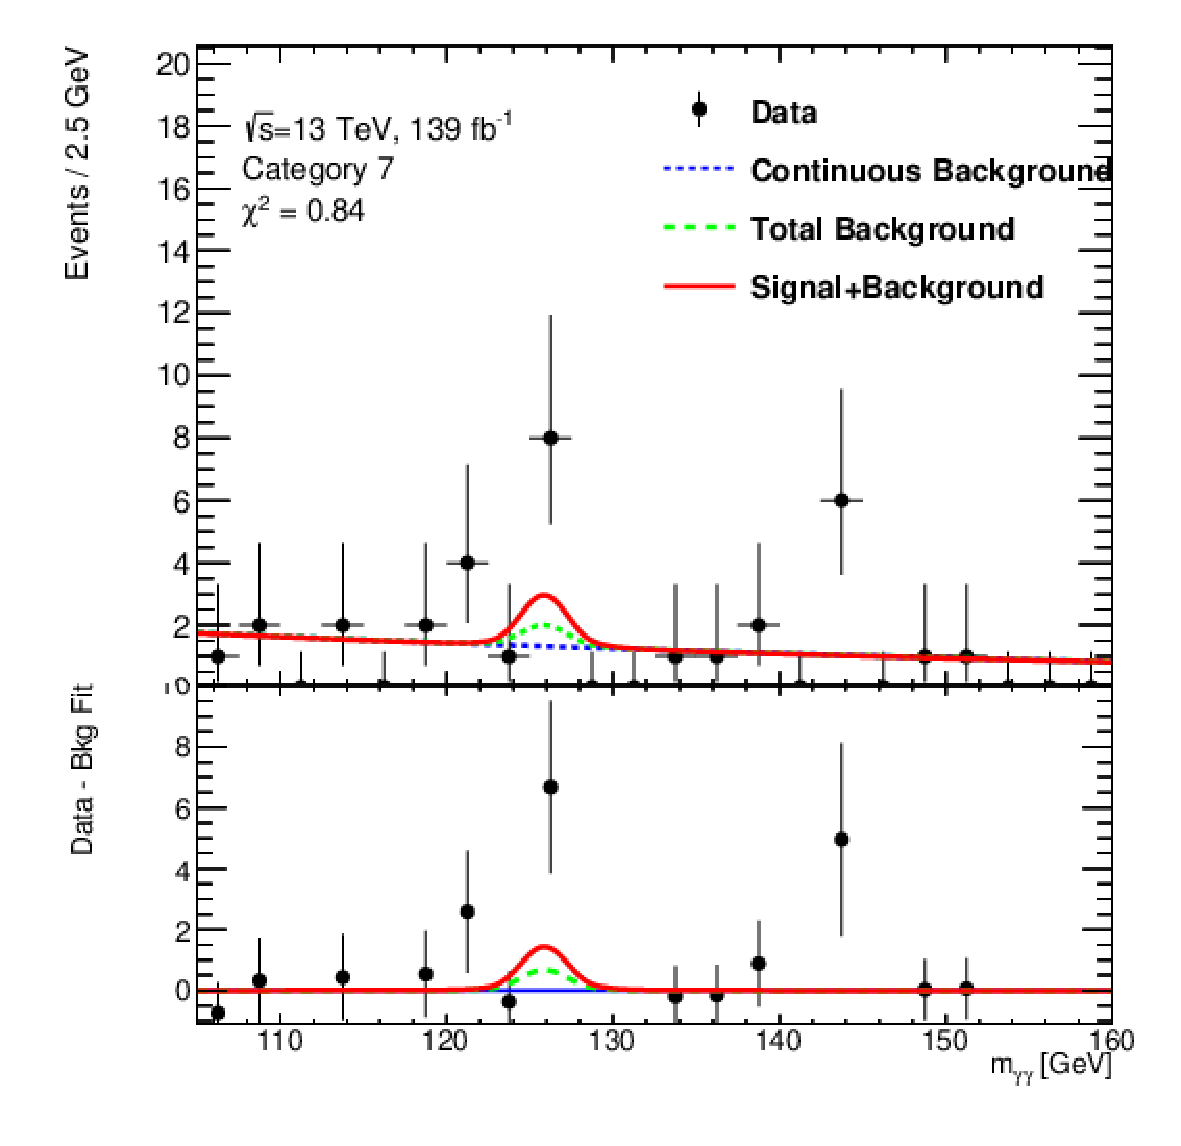
\includegraphics[width=0.3\textwidth]{figures/tthcp_results/Had_3_1.pdf}}
  \subfloat[Category 8: $m_{\gamma\gamma}$ (GeV)]{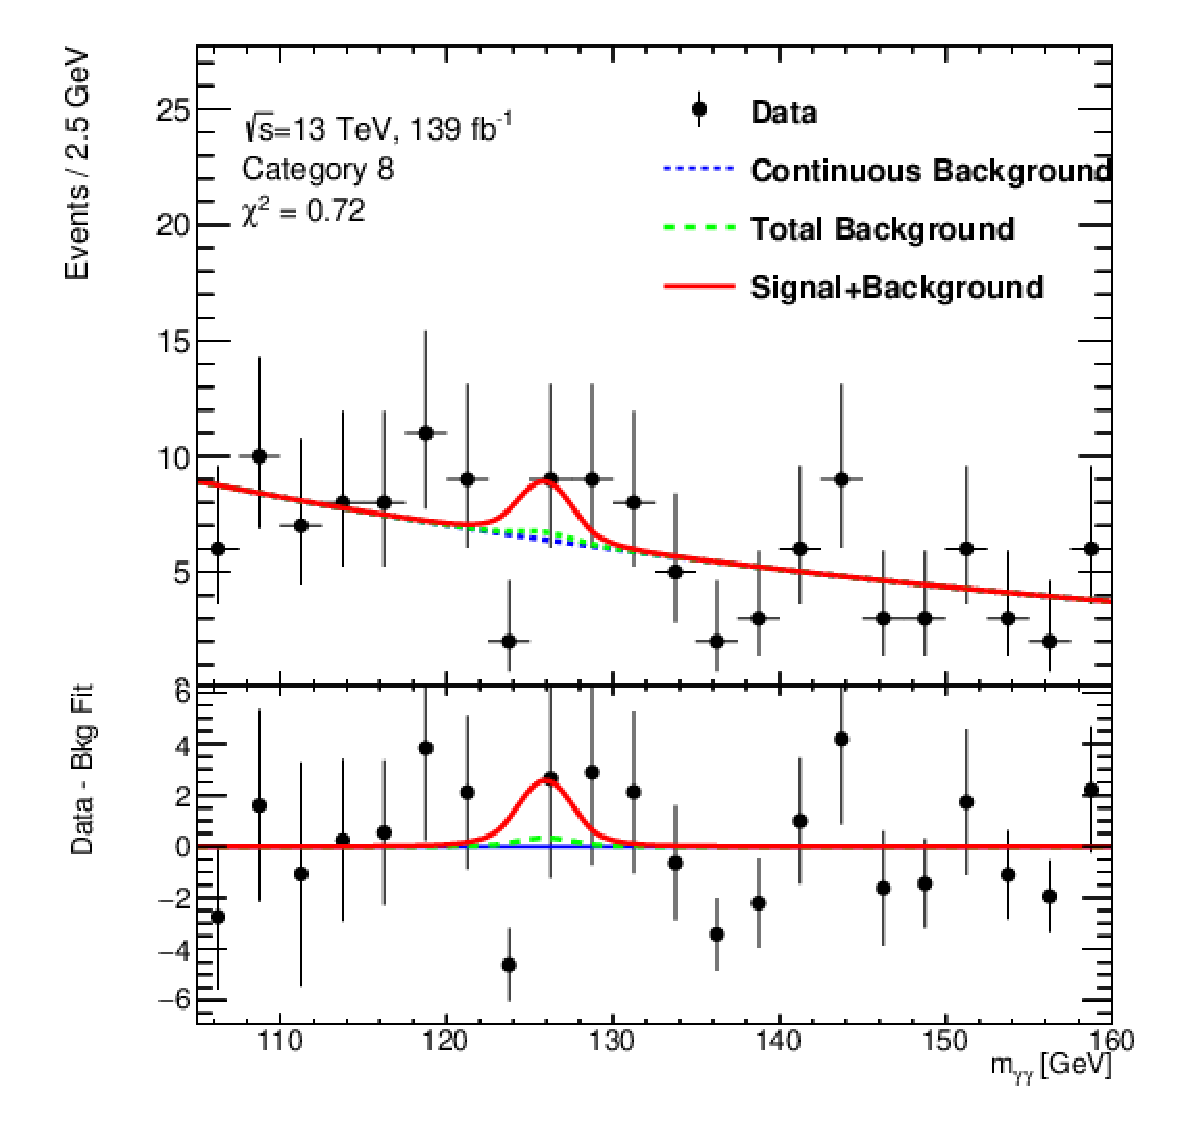
\includegraphics[width=0.3\textwidth]{figures/tthcp_results/Had_3_2.pdf}}
  \subfloat[Category 9: $m_{\gamma\gamma}$ (GeV)]{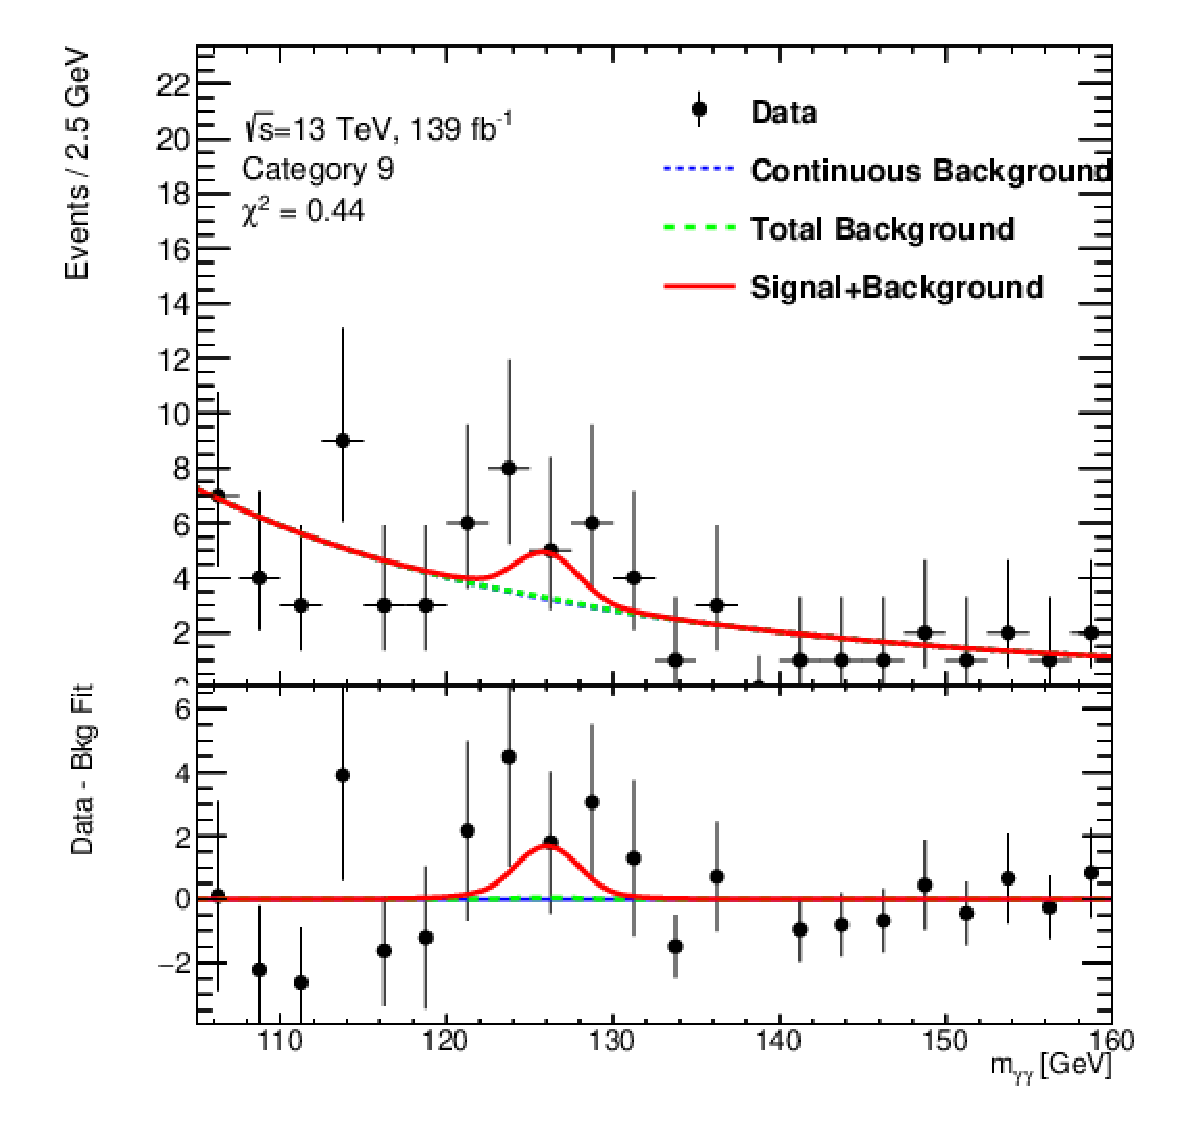
\includegraphics[width=0.3\textwidth]{figures/tthcp_results/Had_3_3.pdf}}\\
  \subfloat[Category 10: $m_{\gamma\gamma}$ (GeV)]{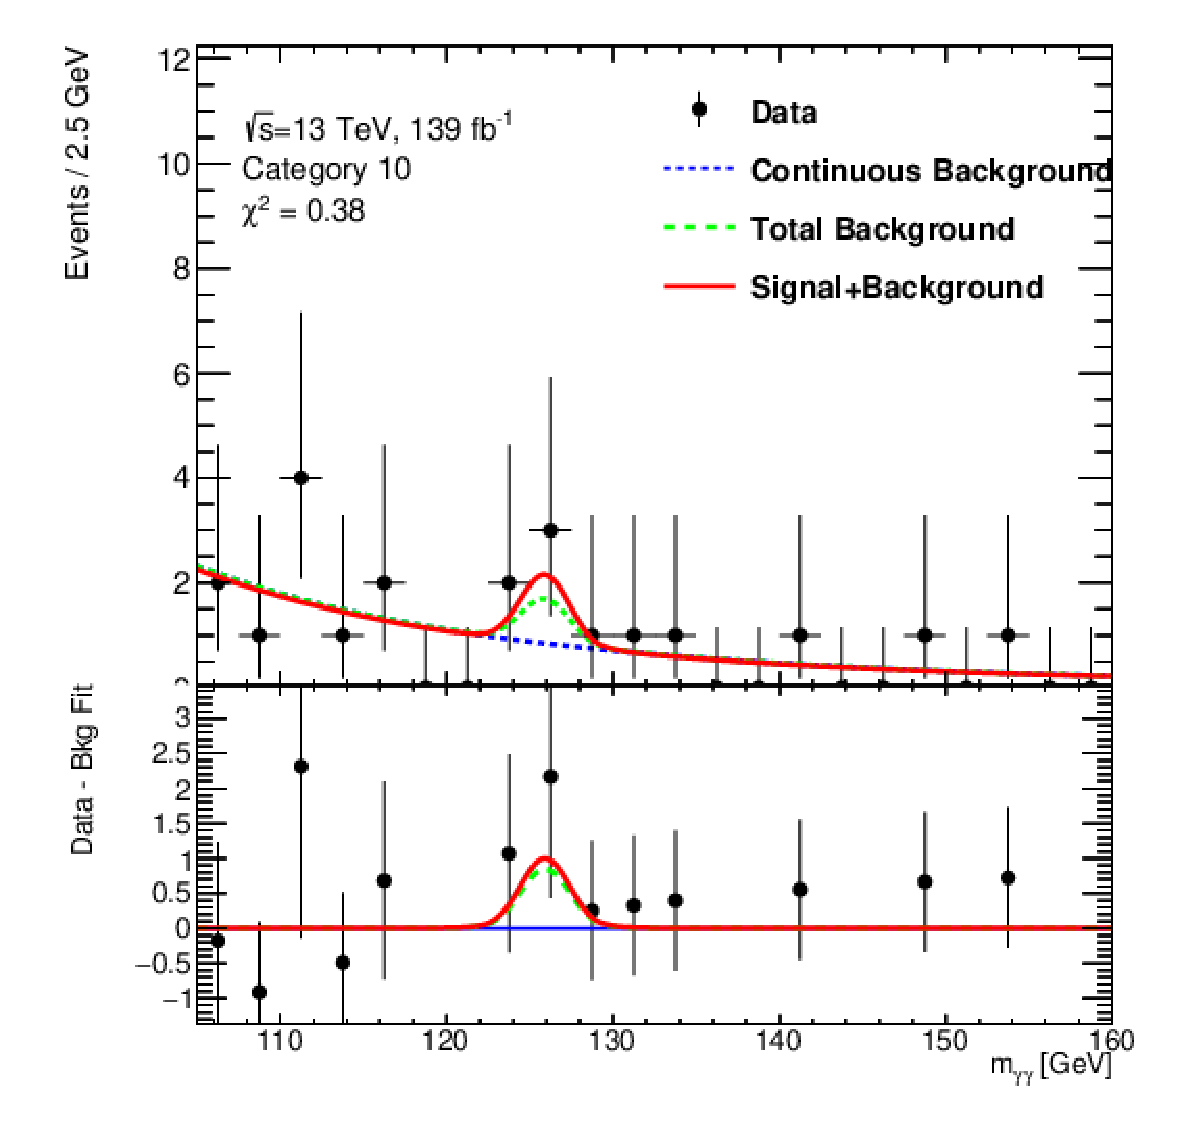
\includegraphics[width=0.3\textwidth]{figures/tthcp_results/Had_4_1.pdf}}
  \subfloat[Category 11: $m_{\gamma\gamma}$ (GeV)]{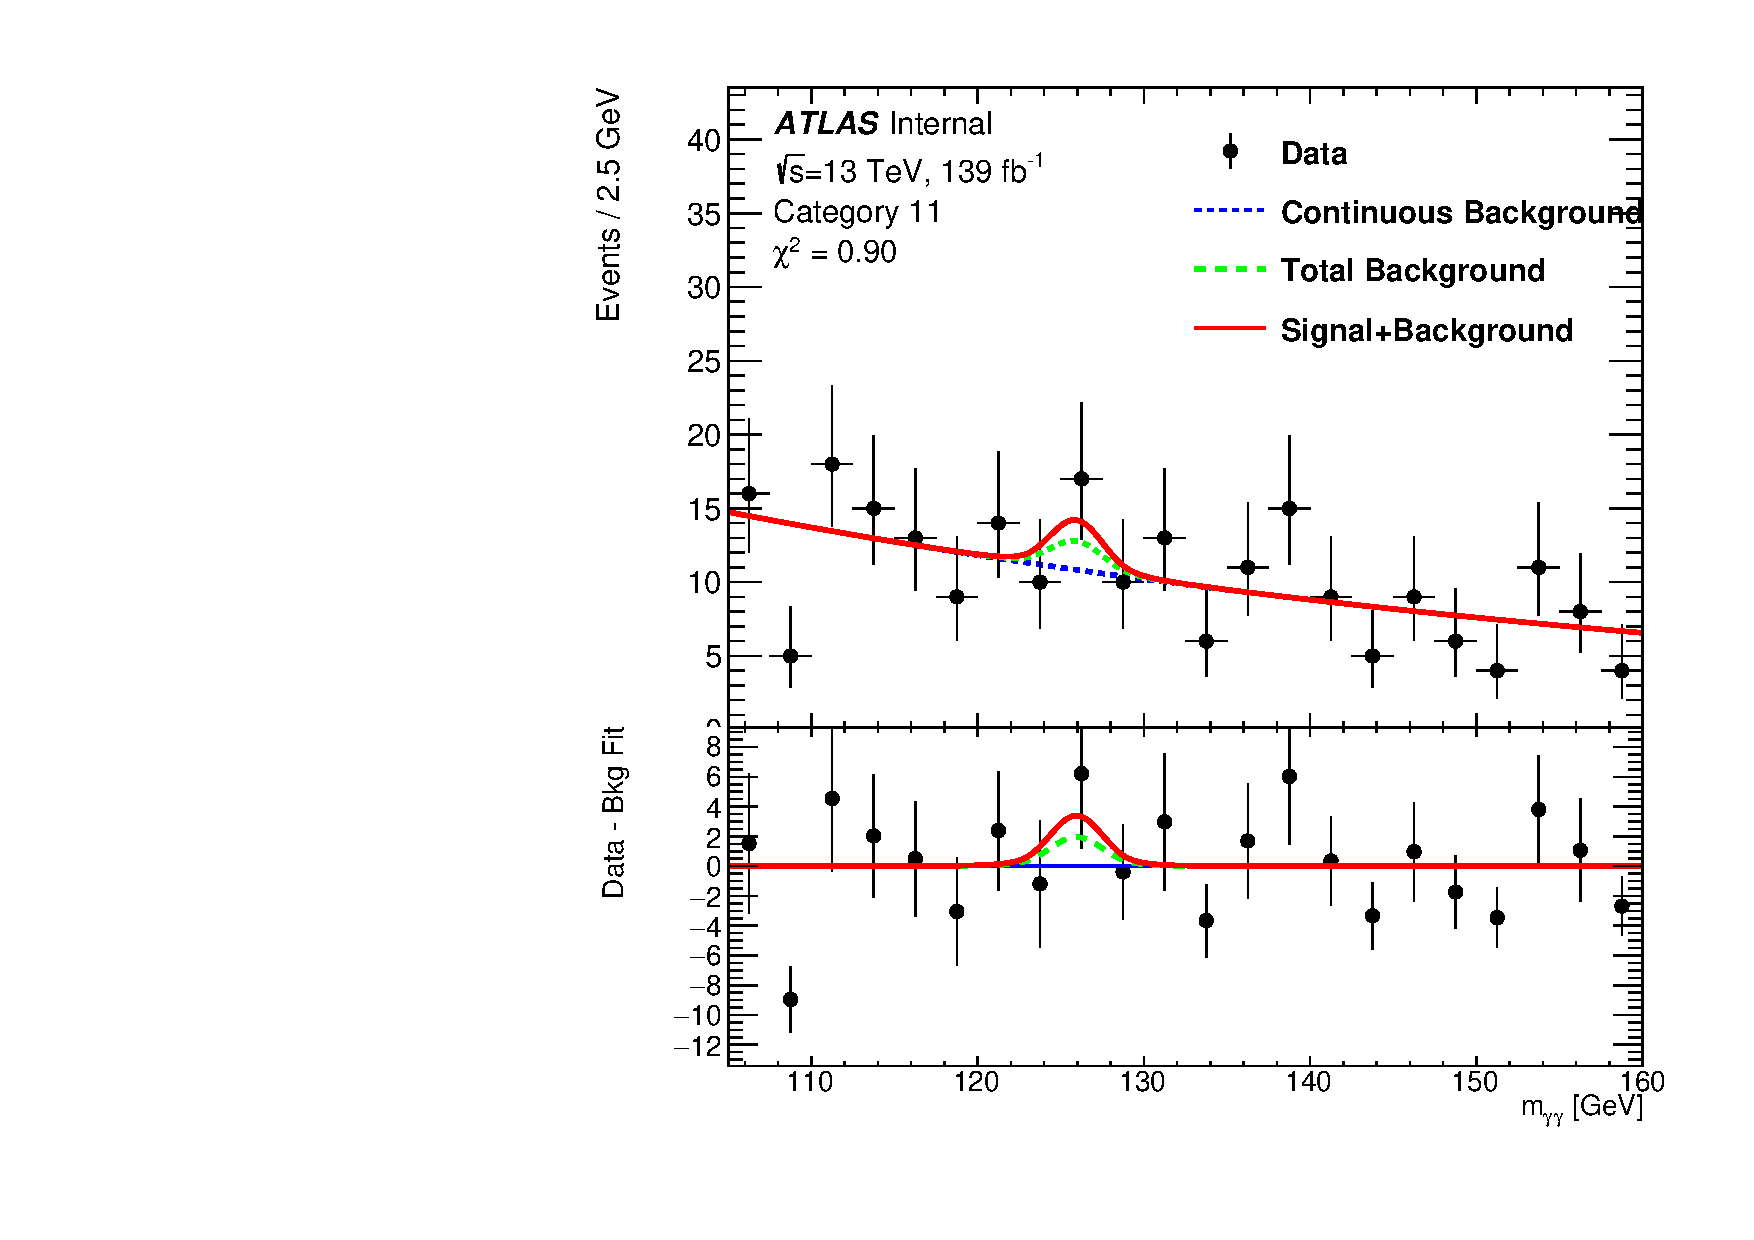
\includegraphics[width=0.3\textwidth]{figures/tthcp_results/Had_4_2.pdf}}
  \subfloat[Category 12: $m_{\gamma\gamma}$ (GeV)]{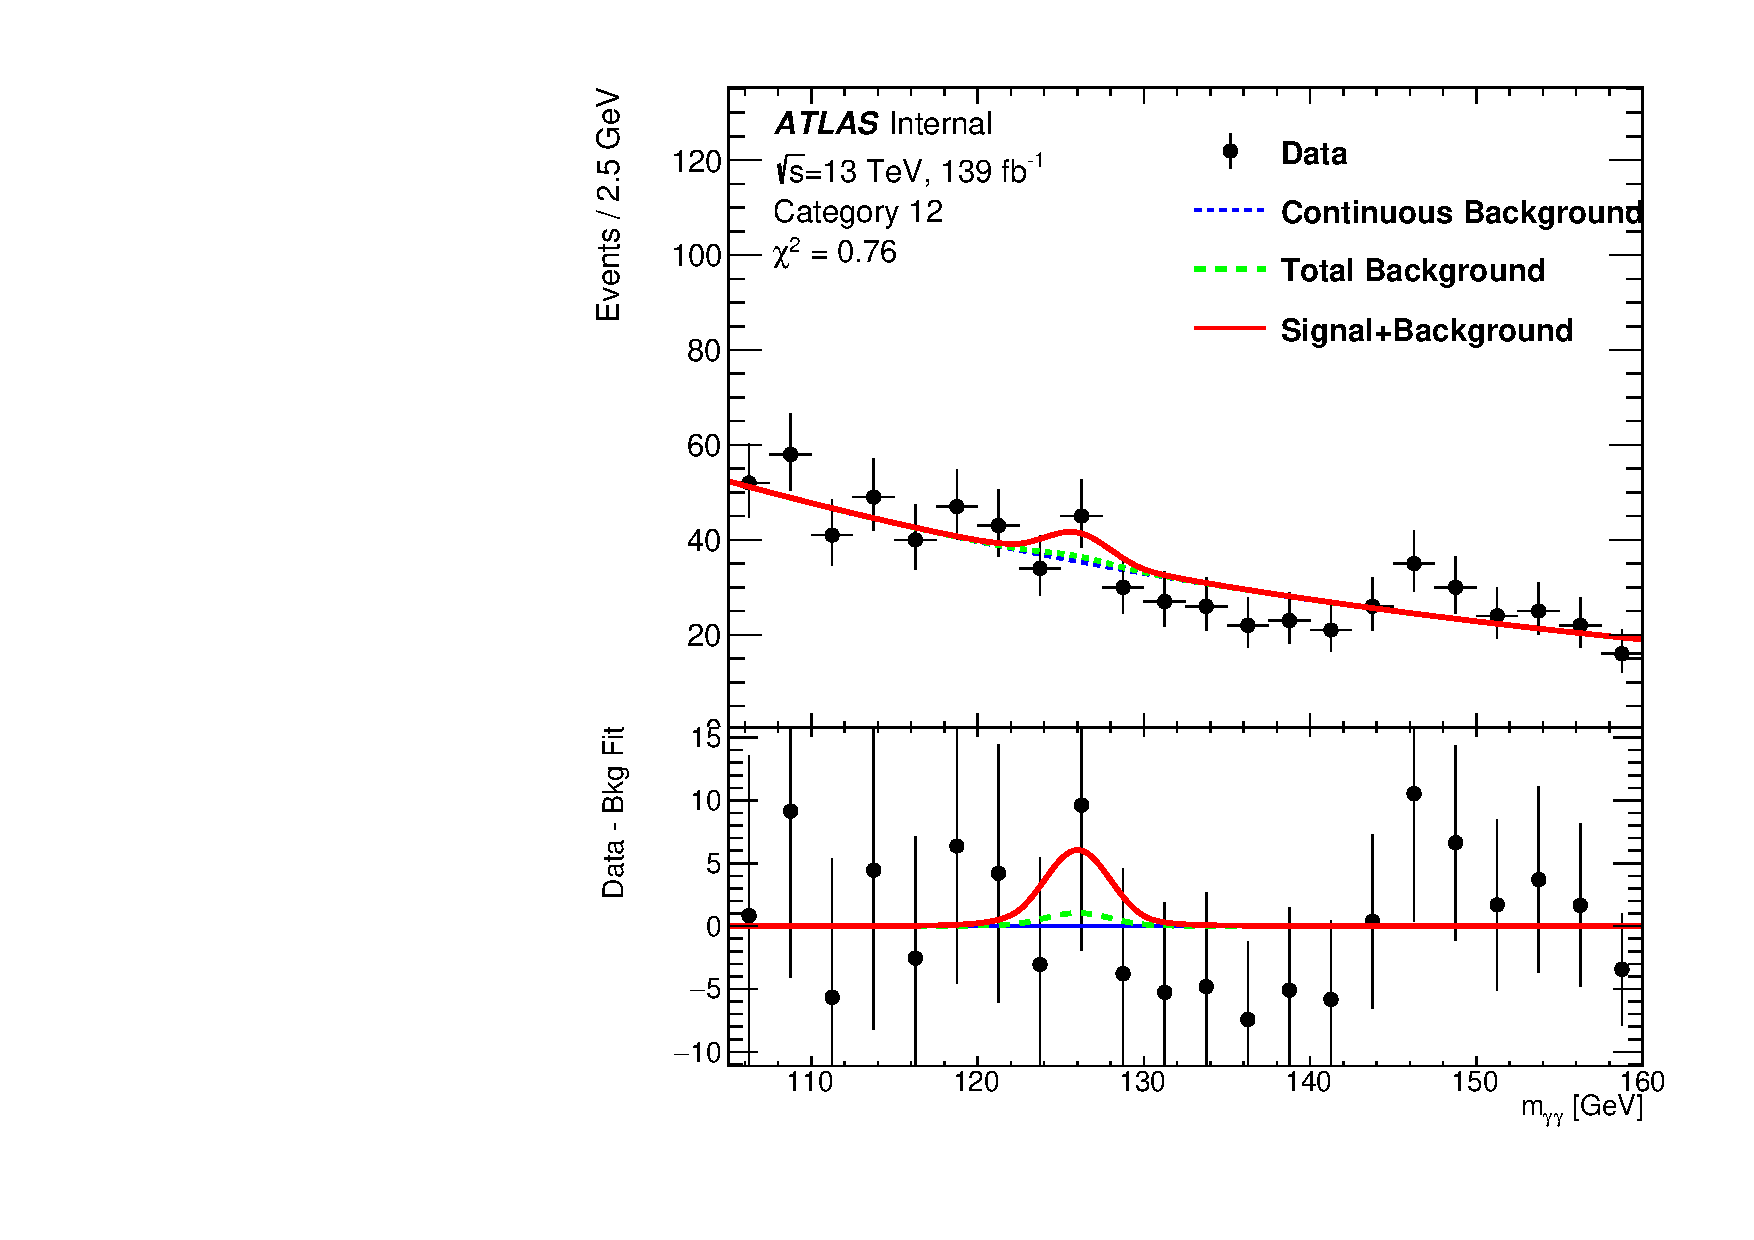
\includegraphics[width=0.3\textwidth]{figures/tthcp_results/Had_4_3.pdf}}
  \caption{Diphoton invariant mass spectrum ($m_{\gamma\gamma}$) in the second six hadronic categories. The fitted continuum background is shown in blue the, total background including non-top Higgs processes is shown in green, and total fitted signal plus background is shown in red.}
  \label{fig:invmass_had2}
\end{figure}

\begin{figure}[htbp]
  \centering
  \subfloat[Category 13: $m_{\gamma\gamma}$ (GeV)]{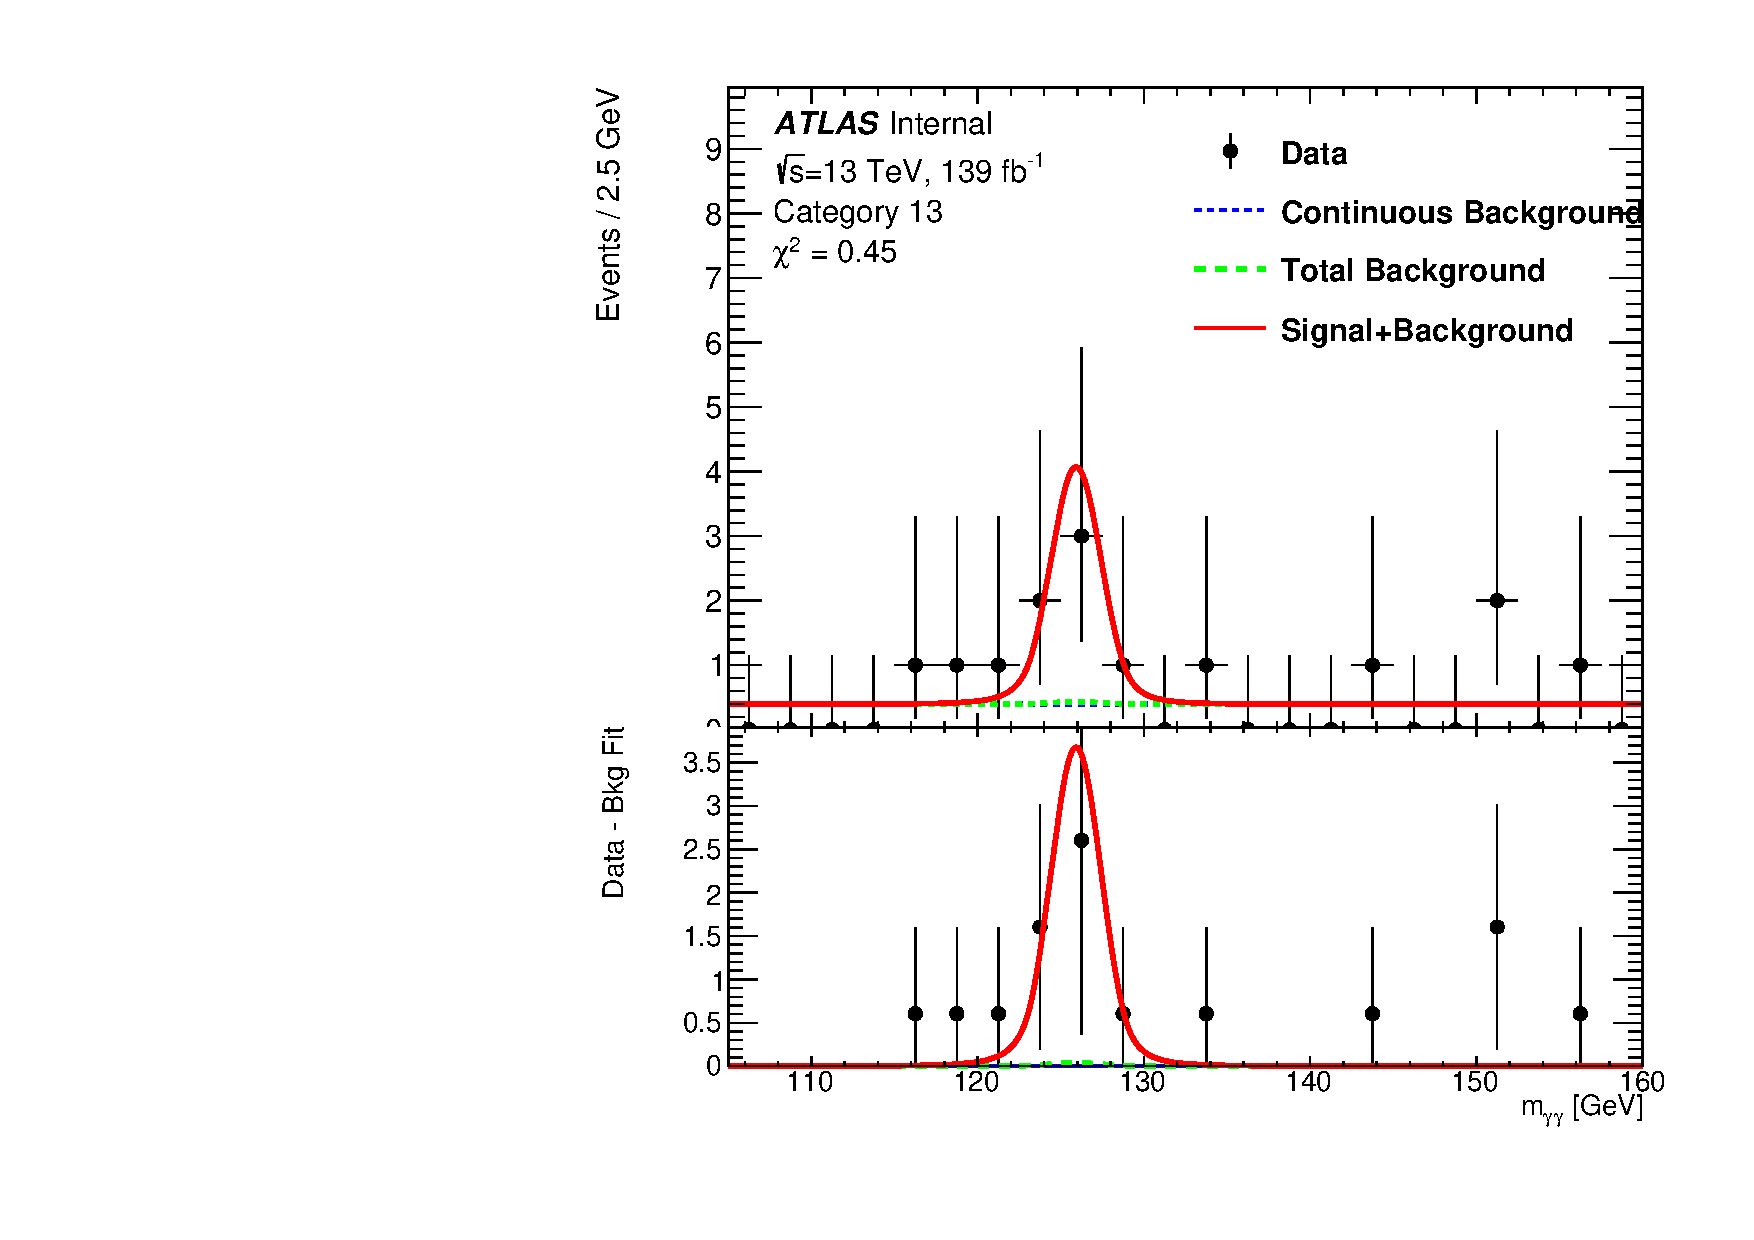
\includegraphics[width=0.3\textwidth]{figures/tthcp_results/Lep_1_1.pdf}}
  \subfloat[Category 14: $m_{\gamma\gamma}$ (GeV)]{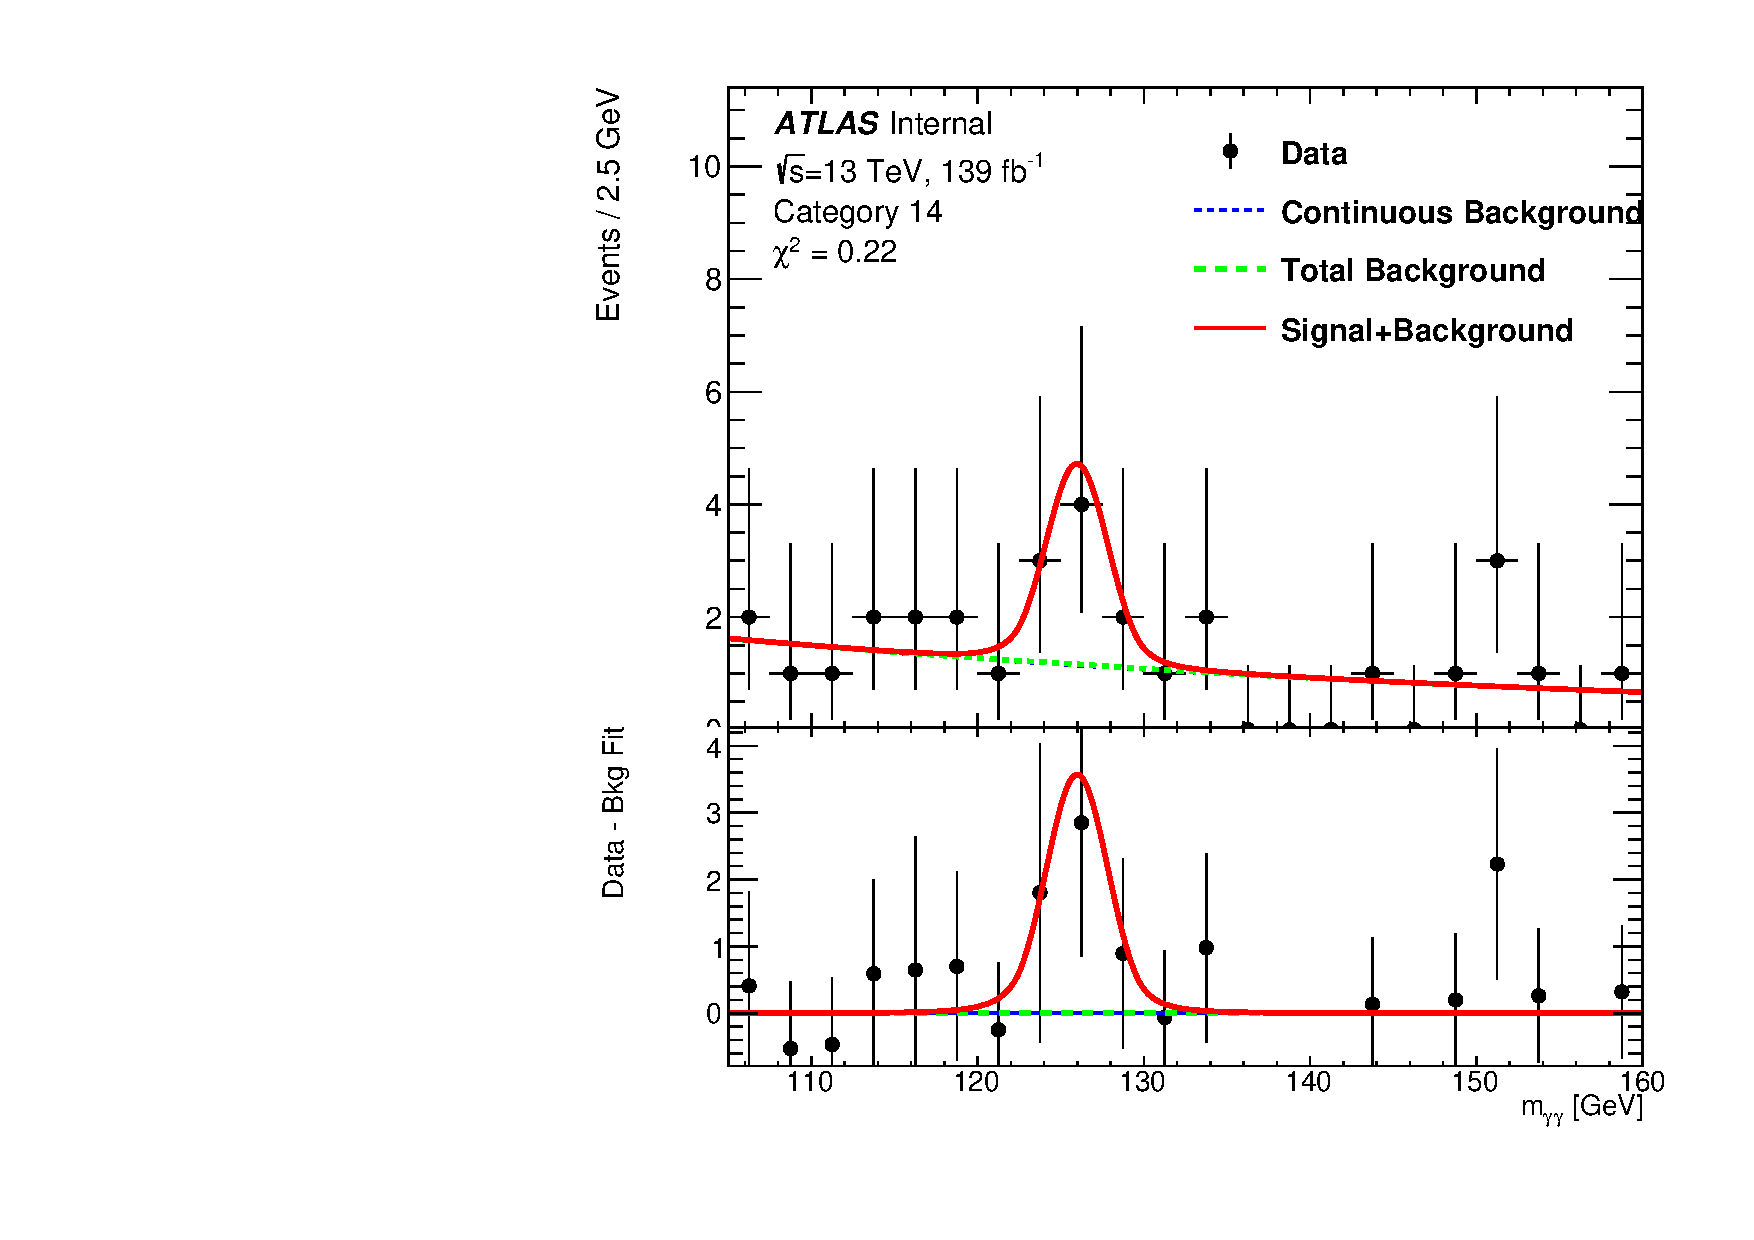
\includegraphics[width=0.3\textwidth]{figures/tthcp_results/Lep_1_2.pdf}}\\
  \subfloat[Category 15: $m_{\gamma\gamma}$ (GeV)]{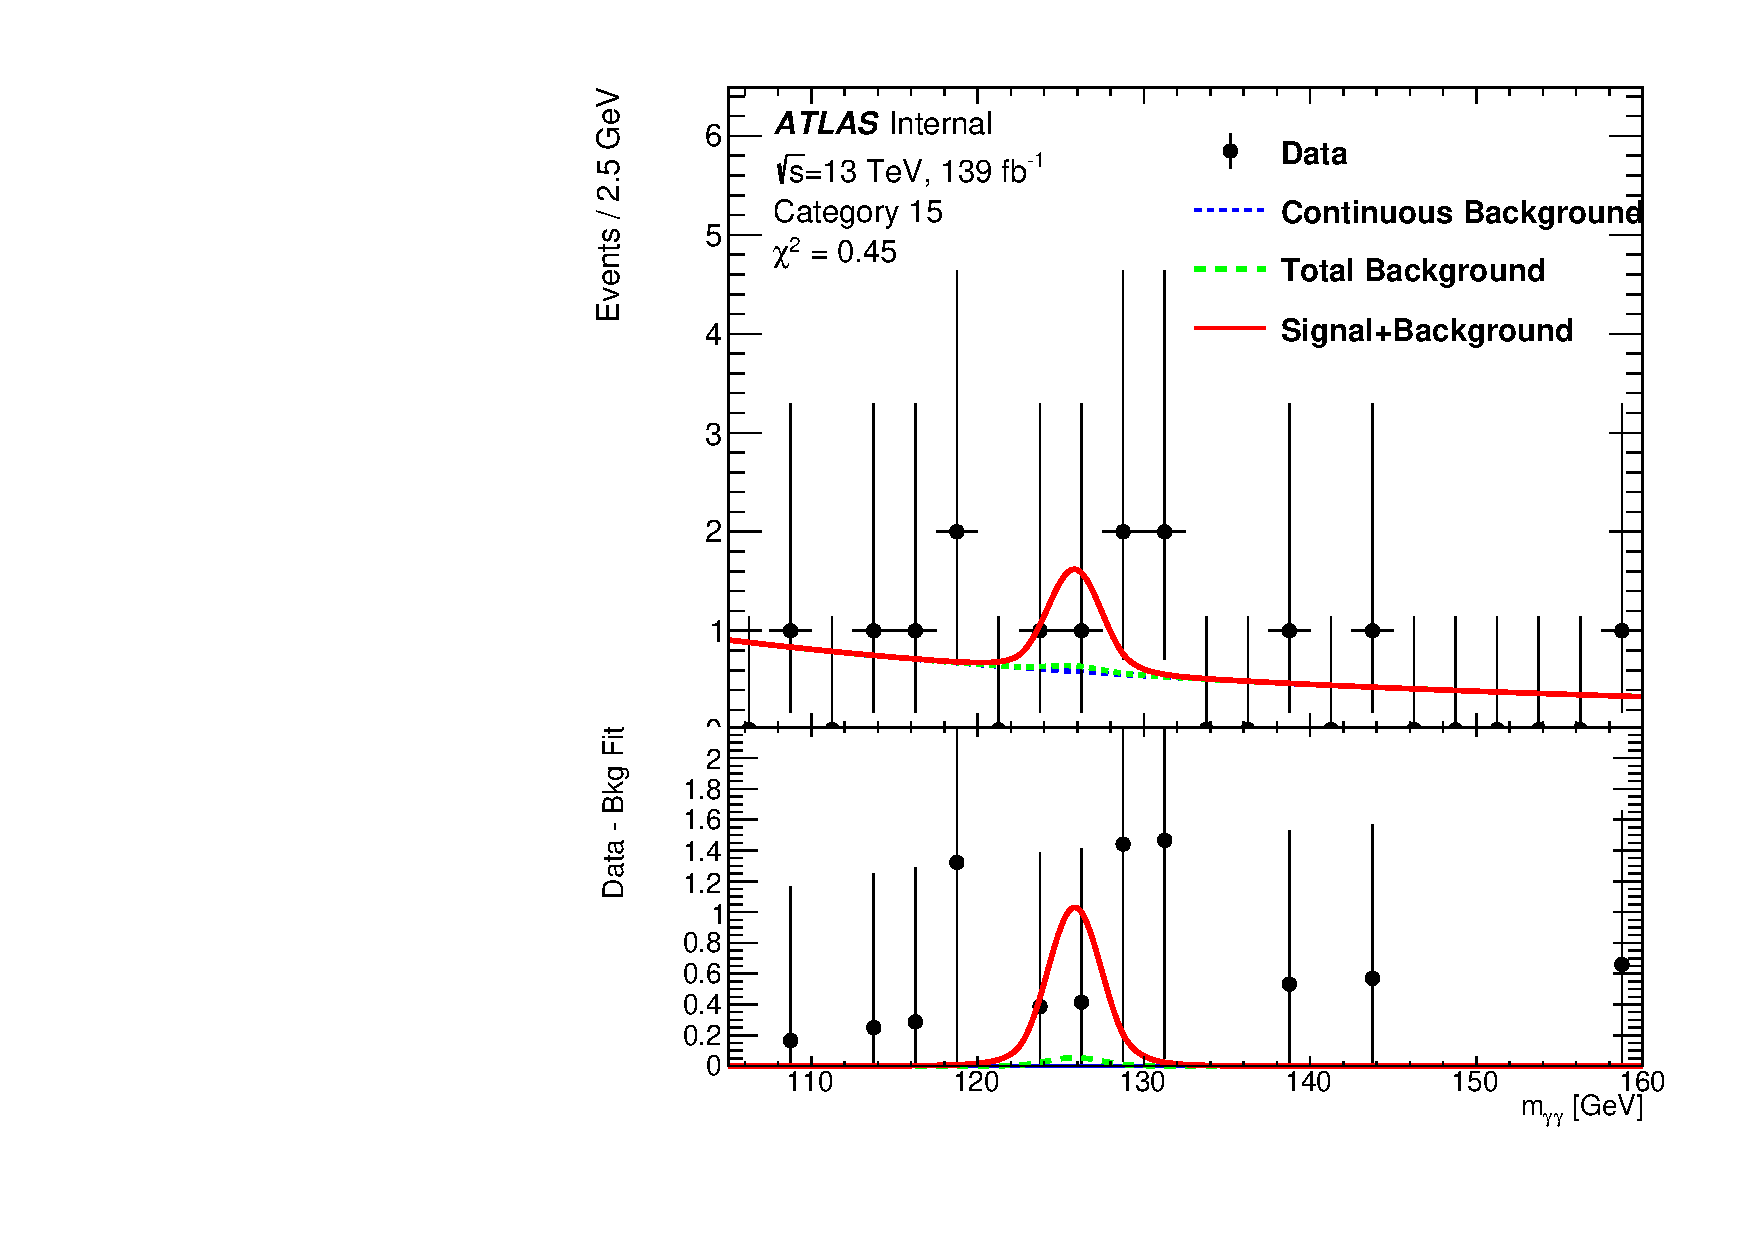
\includegraphics[width=0.3\textwidth]{figures/tthcp_results/Lep_2_1.pdf}}
  \subfloat[Category 16: $m_{\gamma\gamma}$ (GeV)]{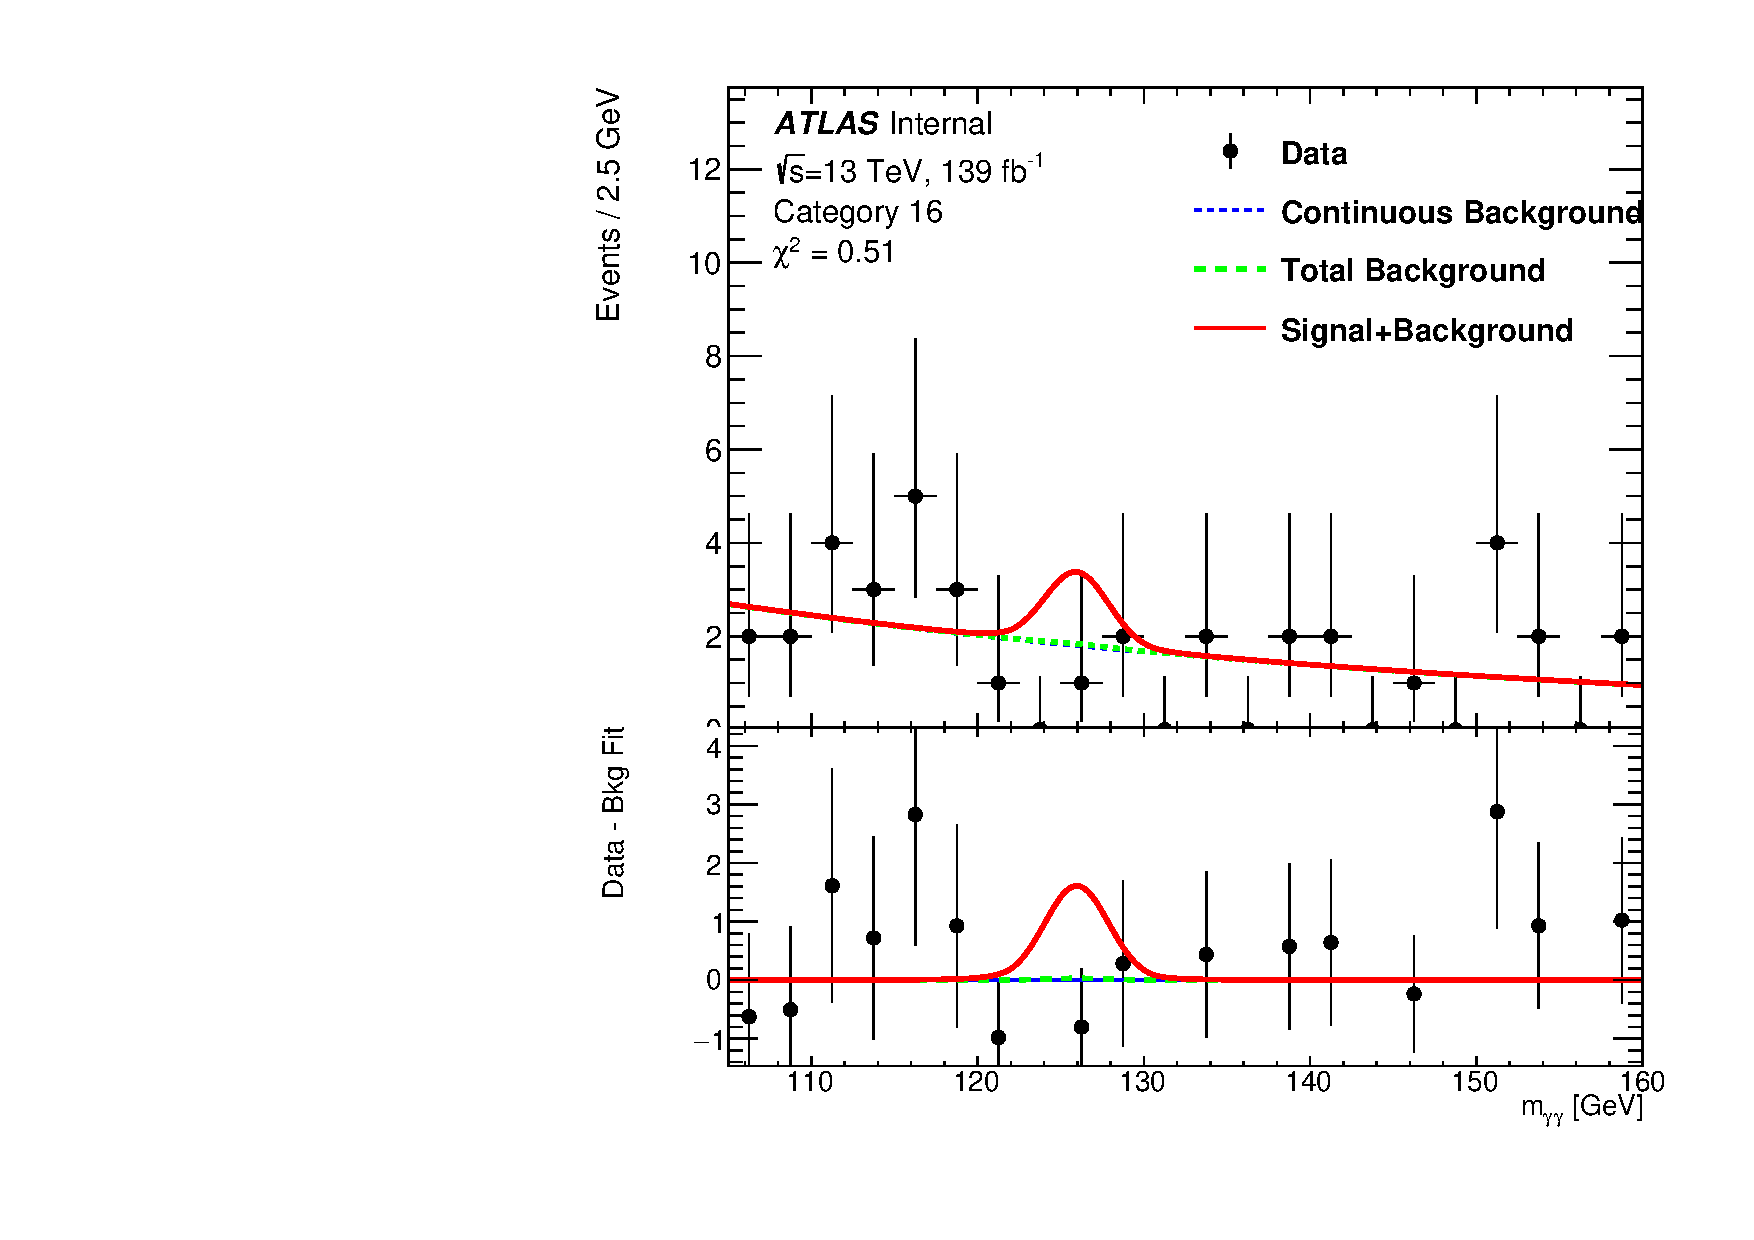
\includegraphics[width=0.3\textwidth]{figures/tthcp_results/Lep_2_2.pdf}}
  \subfloat[Category 17: $m_{\gamma\gamma}$ (GeV)]{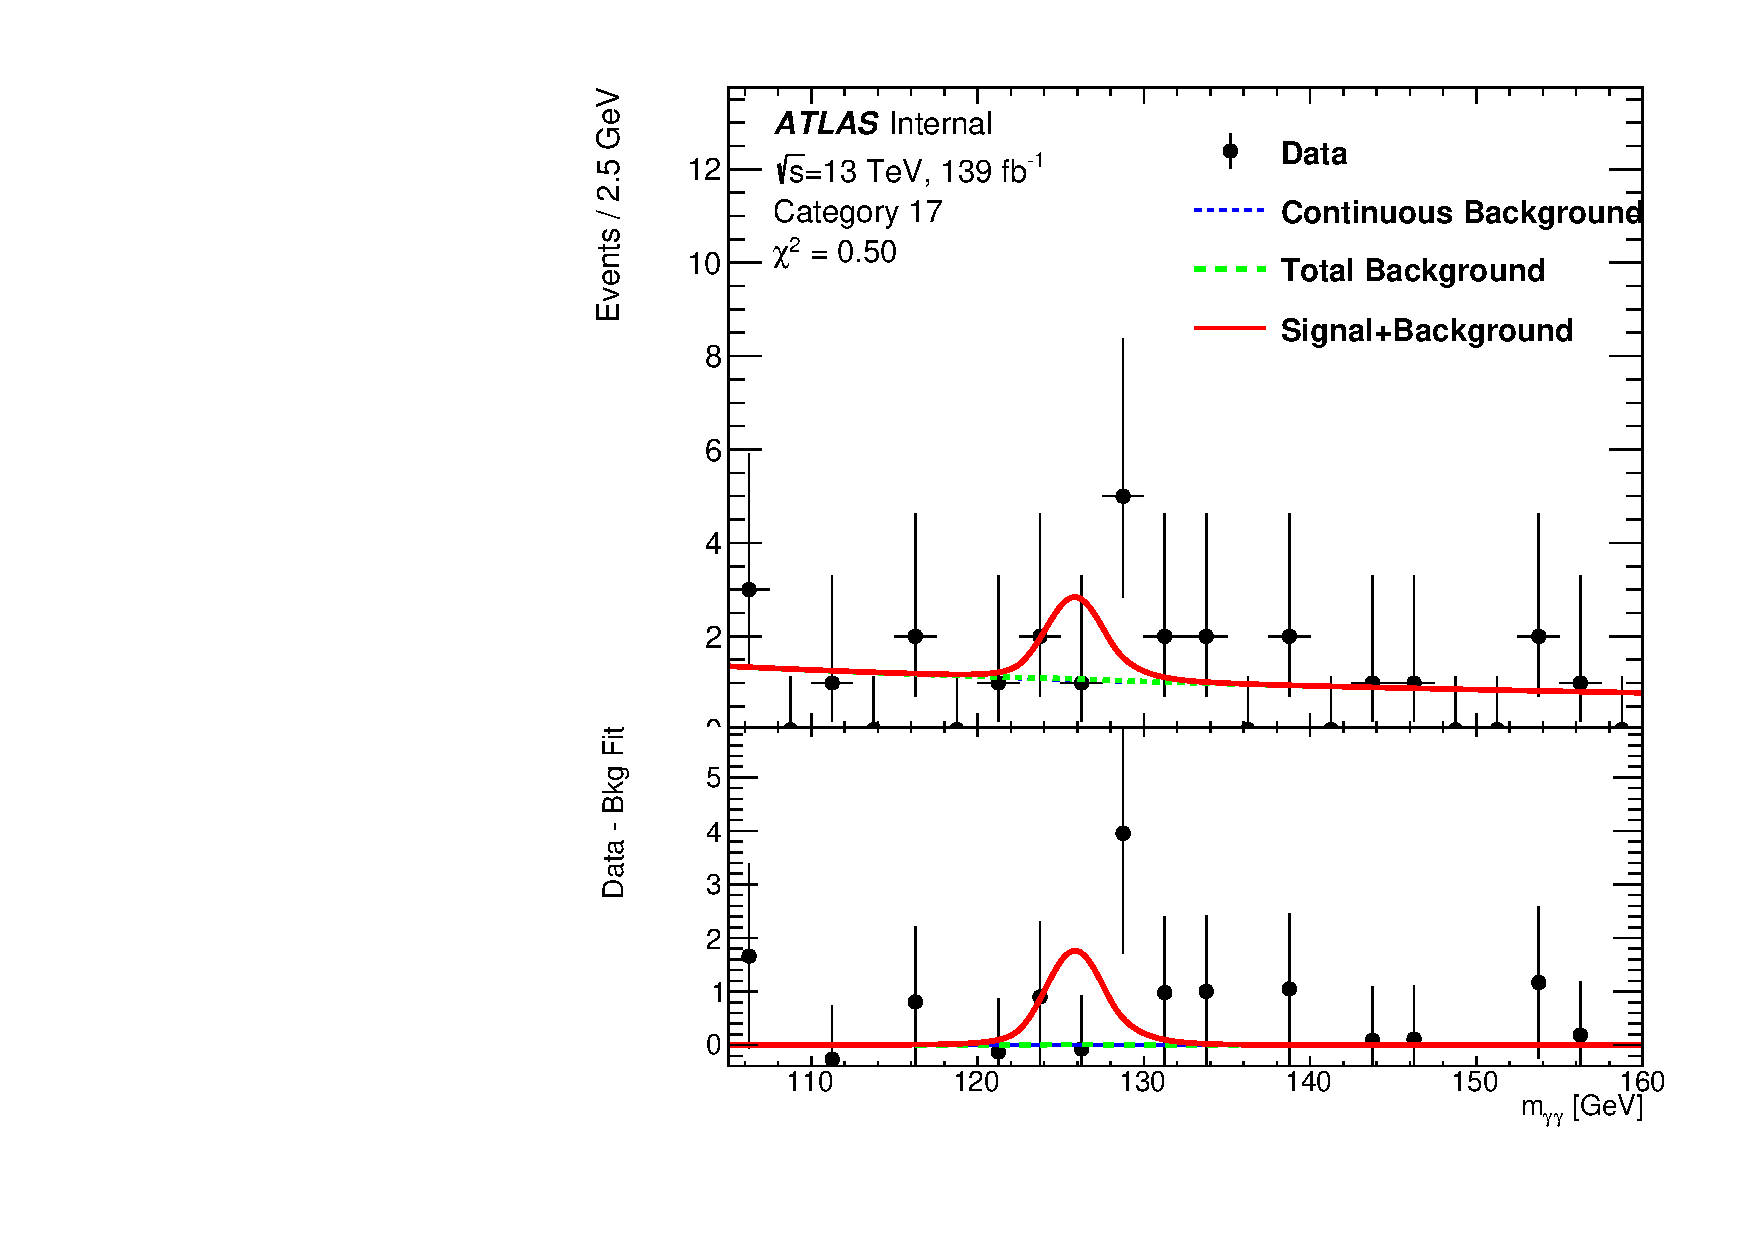
\includegraphics[width=0.3\textwidth]{figures/tthcp_results/Lep_2_3.pdf}}\\
  \subfloat[Category 18: $m_{\gamma\gamma}$ (GeV)]{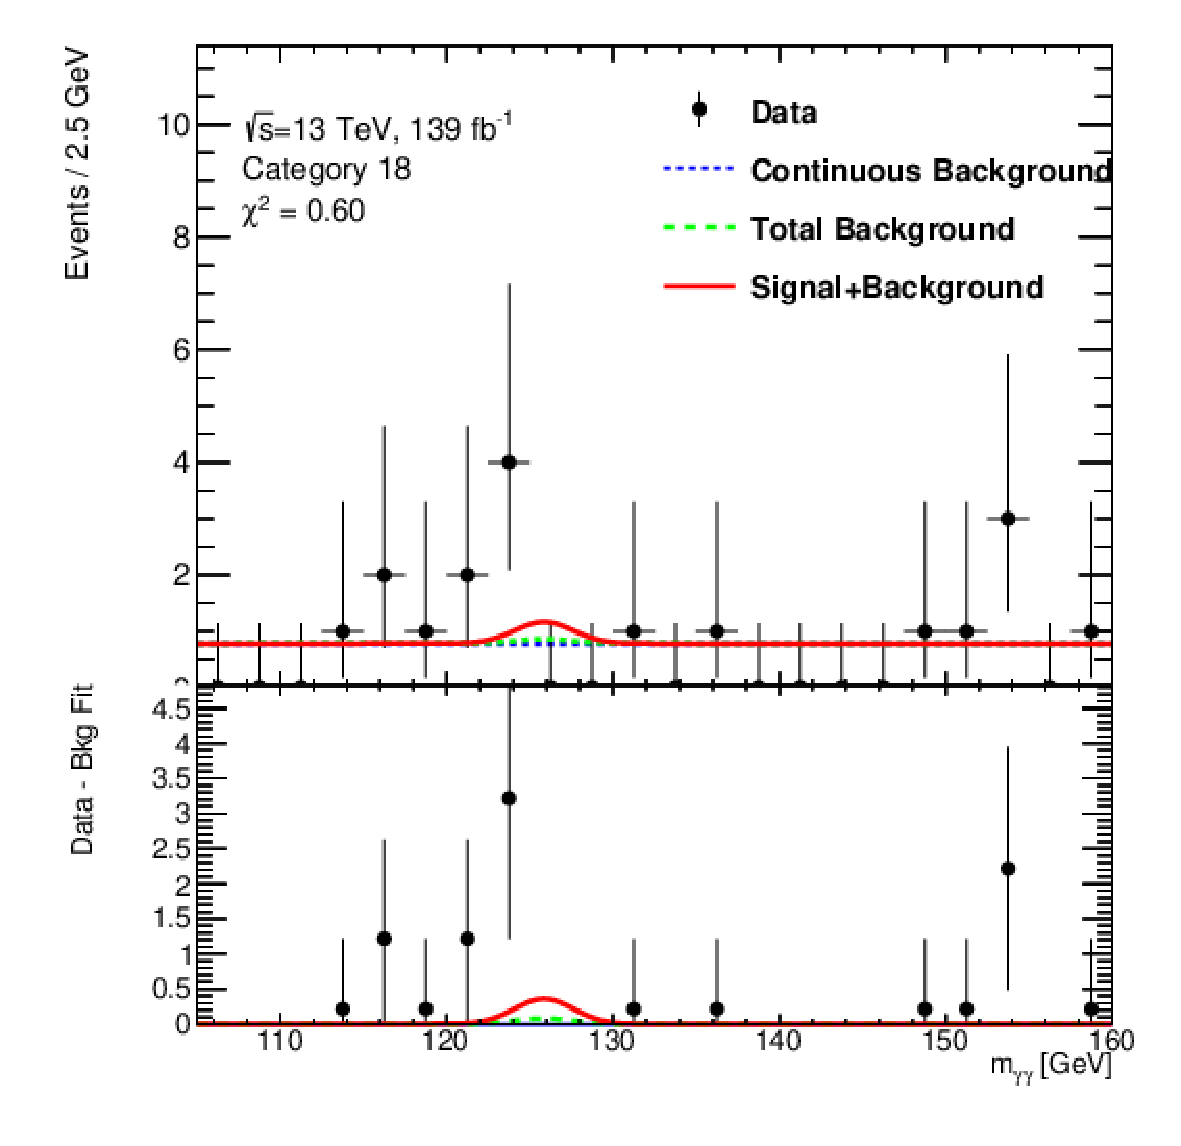
\includegraphics[width=0.3\textwidth]{figures/tthcp_results/Lep_3_1.pdf}}
  \subfloat[Category 19: $m_{\gamma\gamma}$ (GeV)]{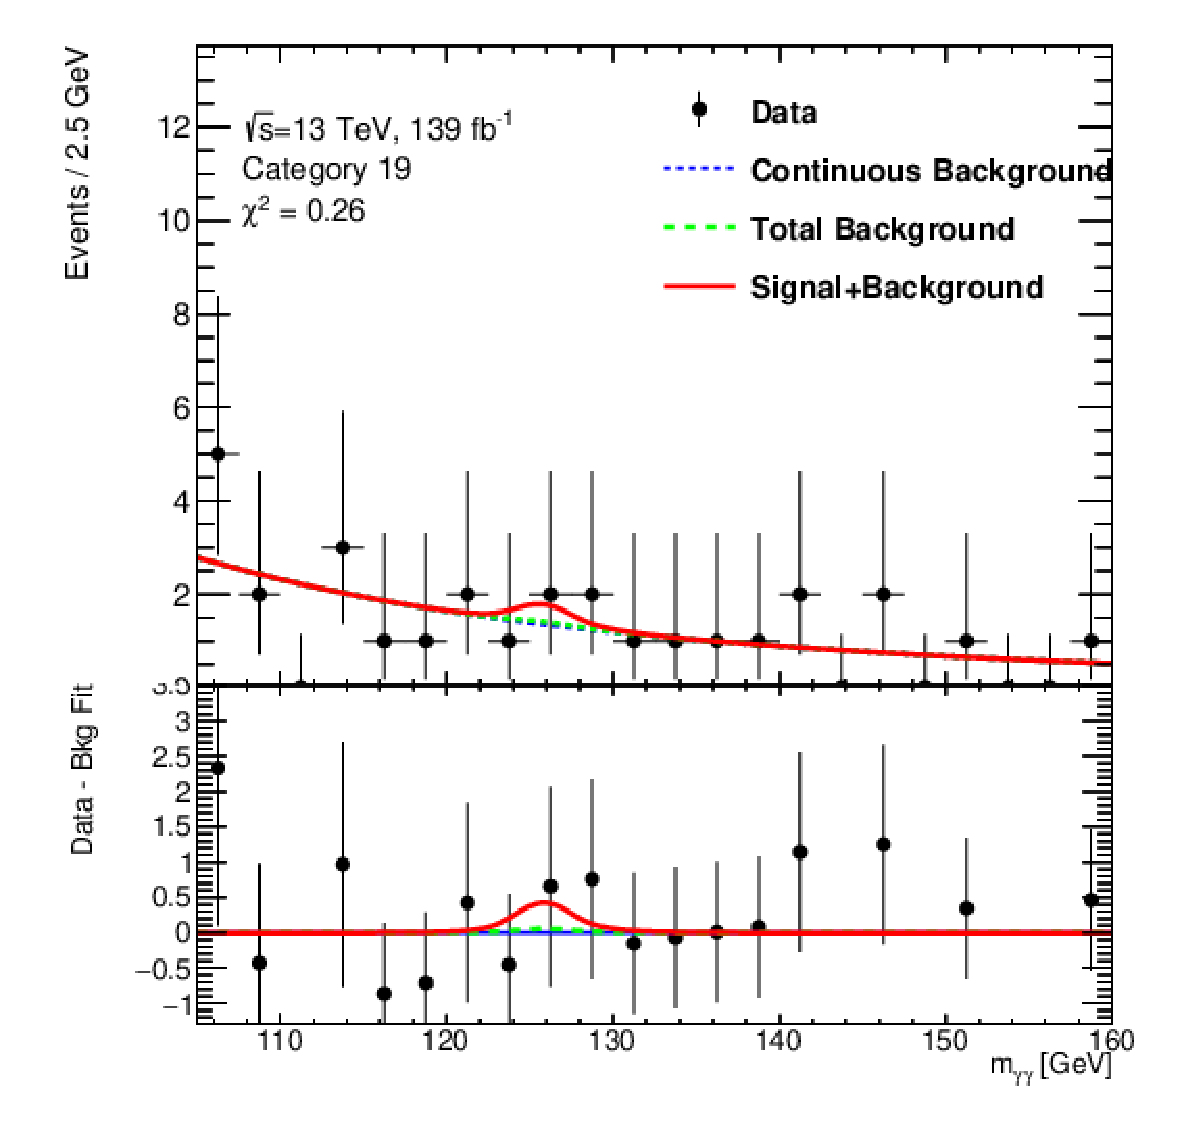
\includegraphics[width=0.3\textwidth]{figures/tthcp_results/Lep_3_2.pdf}}
  \subfloat[Category 20: $m_{\gamma\gamma}$ (GeV)]{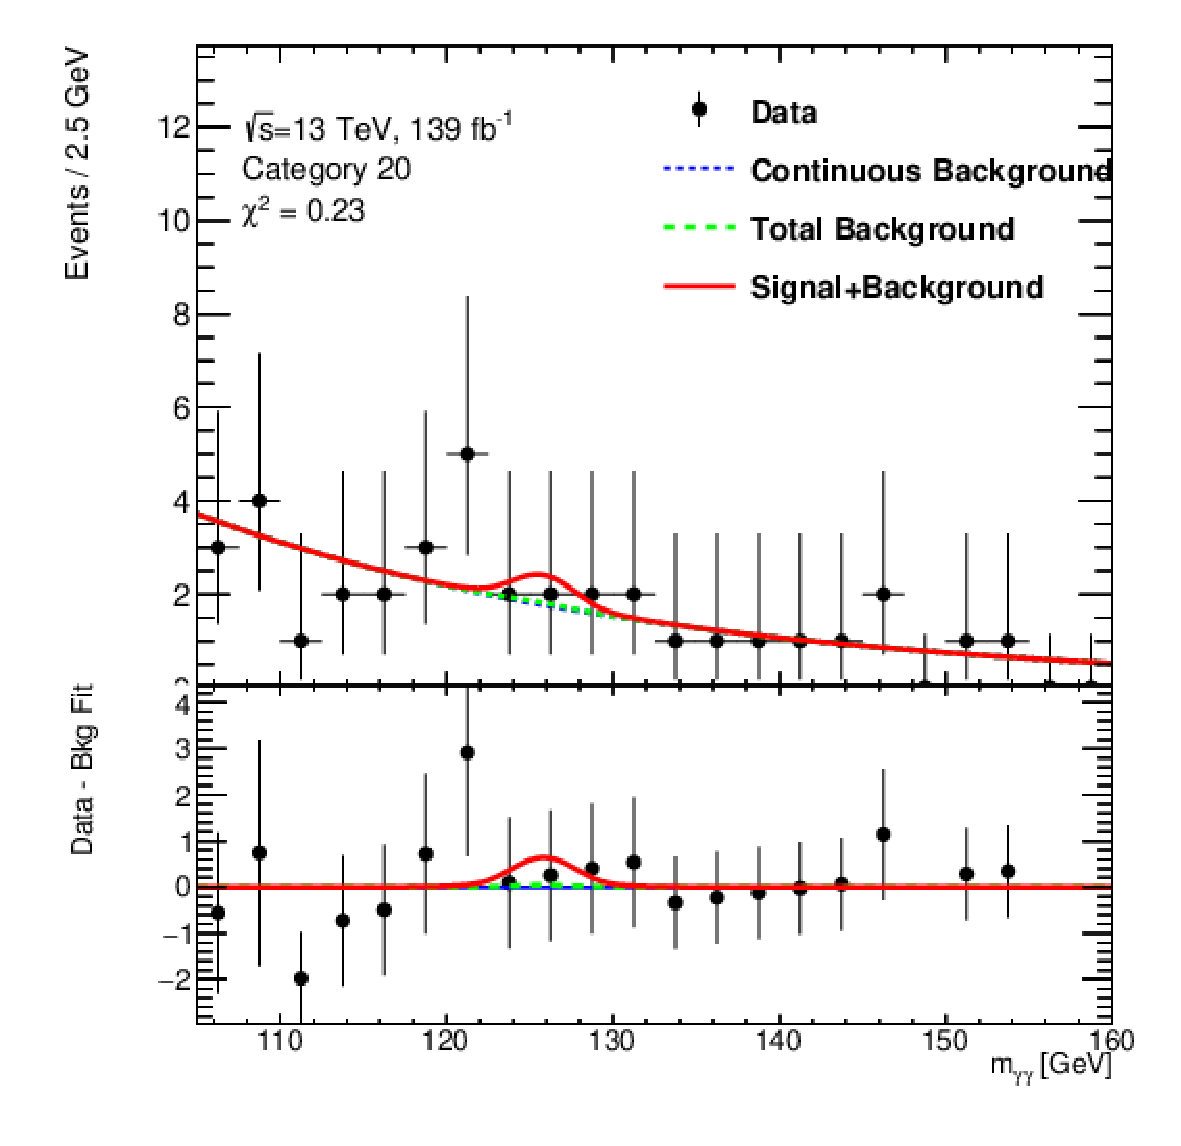
\includegraphics[width=0.3\textwidth]{figures/tthcp_results/Lep_3_3.pdf}}\
  \caption{Diphoton invariant mass spectrum ($m_{\gamma\gamma}$) in the eight leptonic categories. The fitted continuum background is shown in blue the, total background including non-top Higgs processes is shown in green, and total fitted signal plus background is shown in red.}
    \label{fig:invmass_lep}
\end{figure}

\begin{figure}[htbp]
  \centering
  \subfloat[Sum of categories (unweighted): $m_{\gamma\gamma}$ (GeV)]{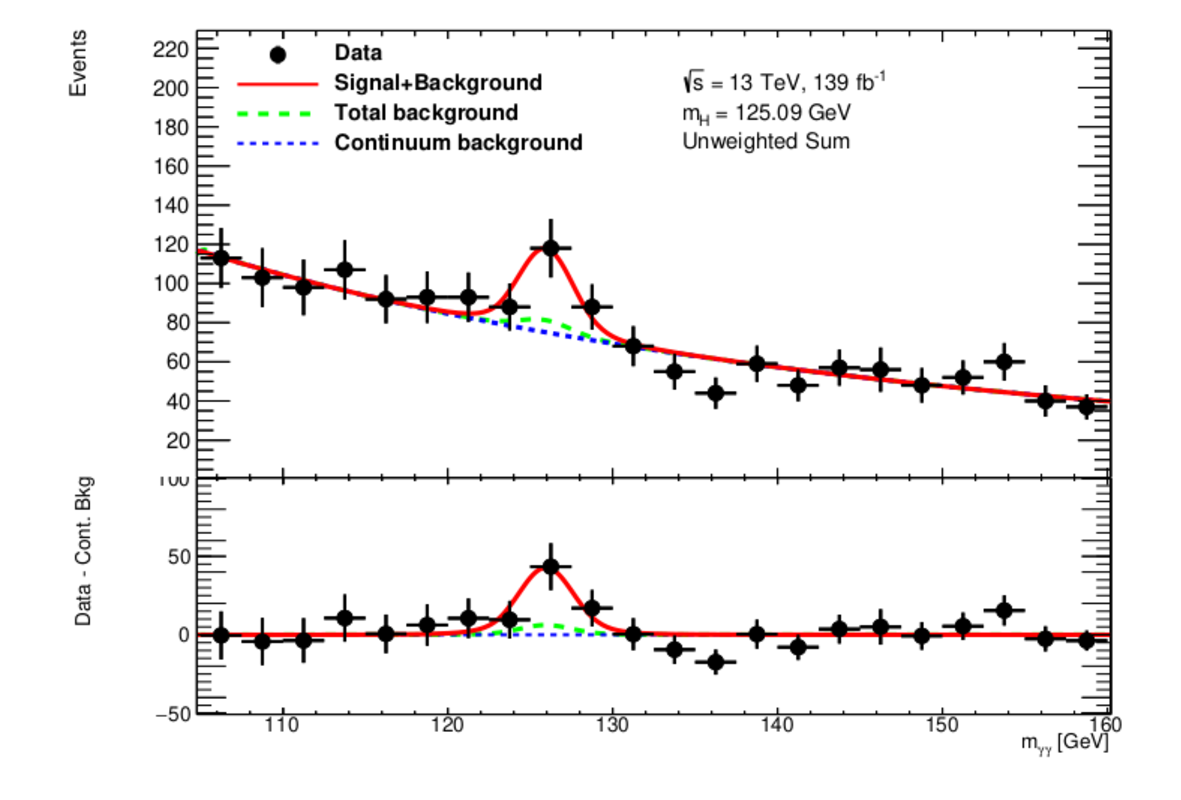
\includegraphics[width=0.3\textwidth]{figures/tthcp_results/hunwt.pdf}}
  \subfloat[Sum of categories (weighted): $m_{\gamma\gamma}$ (GeV)]{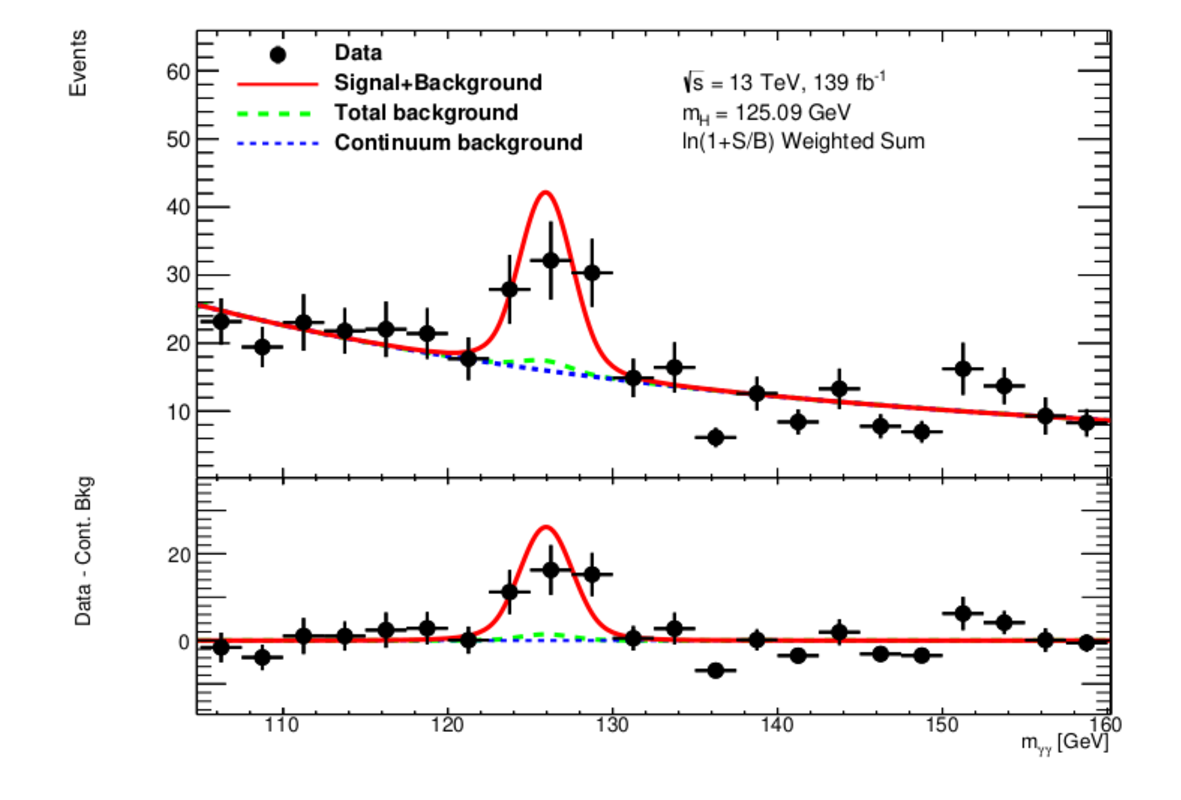
\includegraphics[width=0.3\textwidth]{figures/tthcp_results/hwt.pdf}}
    \caption{The weighted and unweighted sum of all twenty analysis categories. In the weighted plot, events are weighted by $\ln(1+S/B)$, where $S$ and $B$ are calculated in the window $m_H\pm3$ GeV.}
\label{fig:invmass_tot}
\end{figure}



\begin{sidewaystable}[ht]
\begin{center}
\begin{tabular}{ l | ll | ll | ll | l | l | l }
\hline
\multicolumn{1}{p{1.5cm}}{\centering Category} & \multicolumn{2}{p{2.5cm}}{\centering Expected \\$\kappa_t=1$, $\alpha=0^\circ$}&\multicolumn{2}{p{2.5cm}}{\centering Expected \\$\kappa_t=1$, $\alpha=45^\circ$}&  \multicolumn{2}{p{2.5cm}}{\centering Expected \\$\kappa_t=1$, $\alpha=90^\circ$} &\multicolumn{1}{p{2.5cm}}{\centering Expected \\Resonant Bkg} & \multicolumn{1}{p{1.5cm}}{\centering Continuum Bkg} & \multicolumn{1}{p{1.5cm}}{\centering Data} \\ \hline
& $t\bar{t}H$ & $tH$ & $t\bar{t}H$ & $tH$ & $t\bar{t}H$ & $tH$ & & \\ \hline
1 & 2.12 & 0.141 & 2.33 & 0.549 & 2.53 & 1.67 & 0.404 & 1.37 & 0 \\
2 & 3.52 & 0.0665 & 2.42 & 0.125 & 1.35 & 0.377 & 0.121 & 3.92 & 6 \\
3 & 1.59 & 0.00713 & 0.928 & 0.0150 & 0.215 & 0.0396 & 0.0601 & 1.30 & 8 \\
4 & 0.629 & 0.116 & 0.720 & 0.285 & 0.790 & 0.849 & 0.373 & 1.46 & 2 \\
5 & 1.49 & 0.0634 & 1.07 & 0.0906 & 0.627 & 0.281 & 0.226 & 5.36 & 11 \\
6 & 1.61 & 0.0256 & 0.946 & 0.0230 & 0.256 & 0.0709 & 0.100 & 4.36 & 11 \\
7 & 0.515 & 0.117 & 0.601 & 0.389 & 0.701 & 1.16 & 1.06 & 2.53 & 9  \\
8 & 2.27 & 0.123 & 1.66 & 0.224 & 1.04 & 0.593 & 0.418 & 15.22 & 16 \\
9 & 1.95 & 0.04626 & 1.143 & 0.0454 & 0.311 & 0.106& 0.110 & 8.35 & 20 \\
10 & 0.0943 & 0.0636 & 0.121 & 0.303 & 0.146 & 1.02 & 1.53 & 1.58 & 5 \\
11 & 1.08 & 0.376 & 1.15 & 0.796 & 1.22 & 2.35 & 2.65 & 23.70 & 31 \\
12 & 5.76 & 0.385 & 3.74 & 0.518 & 1.72 & 1.40 & 1.77 & 93.51 & 104 \\ \hline
13 & 2.89 & 0.152 & 2.70 & 0.416 & 2.55 & 1.21 & 0.0424 & 0.789 & 5 \\
14 & 3.93 & 0.0519 & 2.43 & 0.0734 & 0.862 & 0.175 & 0.0130 & 2.86 & 8 \\
15 & 0.728 & 0.195 & 0.750 & 0.463 & 0.778 & 1.34 & 0.0749 & 1.30 & 3 \\
16 & 1.75 & 0.127 & 1.26 & 0.174 & 0.759 & 0.496 & -0.0298 & 4.54 & 3 \\
17 & 1.86 & 0.0481 & 1.12 & 0.0574 & 0.349 & 0.110 & 0.0237 & 2.93 & 4 \\
18 & 0.181 & 0.148 & 0.168 & 0.364 & 0.152 & 1.17 & 0.166 & 1.783 & 4 \\
19 & 0.324 & 0.117 & 0.249 & 0.183 & 0.174 & 0.446 & 0.0922 & 3.70 & 4 \\
20 & 0.683 & 0.0788 & 0.427 & 0.07941 & 0.177 & 0.212 & 0.0759 & 4.75 & 5 \\
\hline
\end{tabular}

\end{center}
\vspace{-0.5cm}
\caption{Observed and expected $t\bar{t}H$ and $tH=tHjb+tWH$ yields per category, calculated in the smallest $m_{\gamma\gamma}$ window containing 90\% of the fitted signal. Expected yields assume $\kappa_{t}=1$.}
\label{tab:yields}
\end{sidewaystable}

\begin{figure}[htbp]
  \centering
\subfloat[Expected Signal]{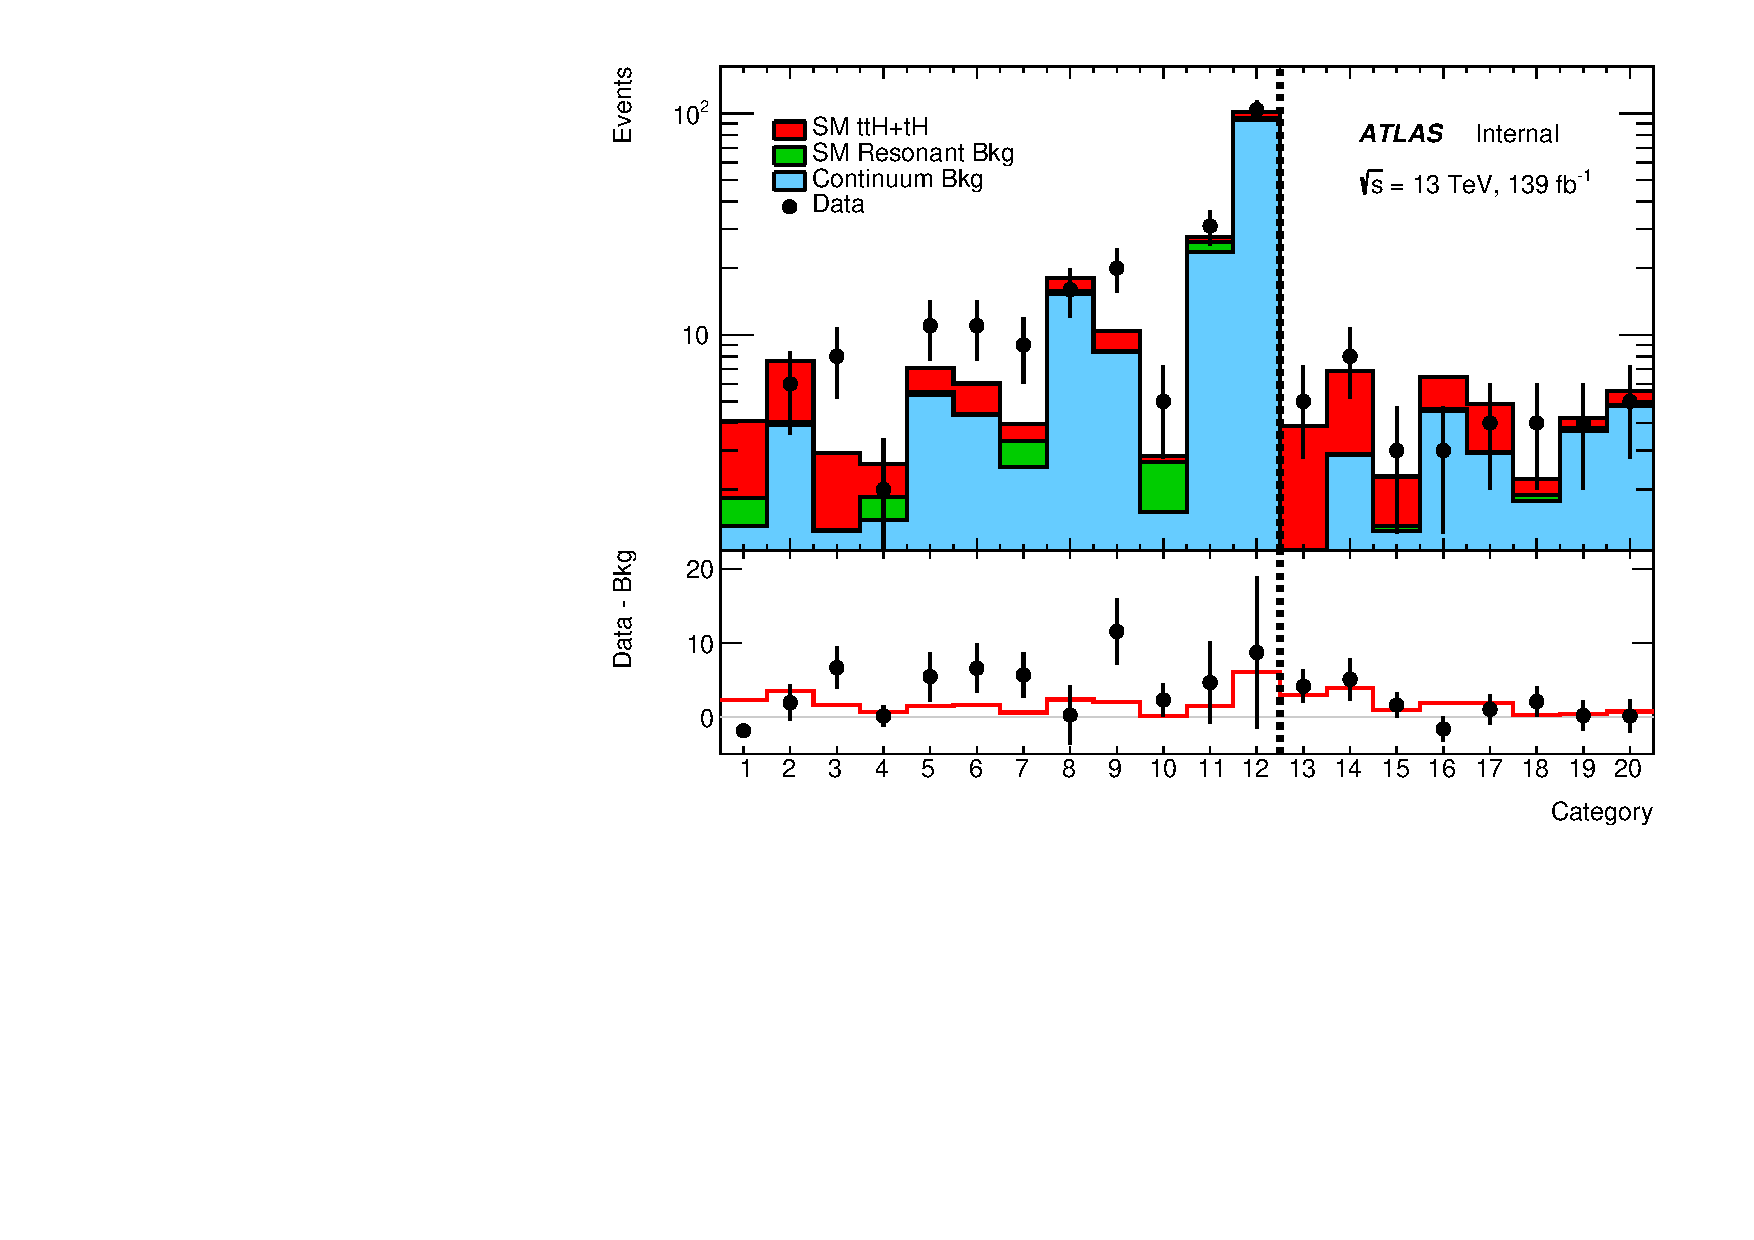
\includegraphics[width=0.6\textwidth]{figures/tthcp_results/yield_S90_exp.pdf}}\\
\subfloat[Fitted Signal]{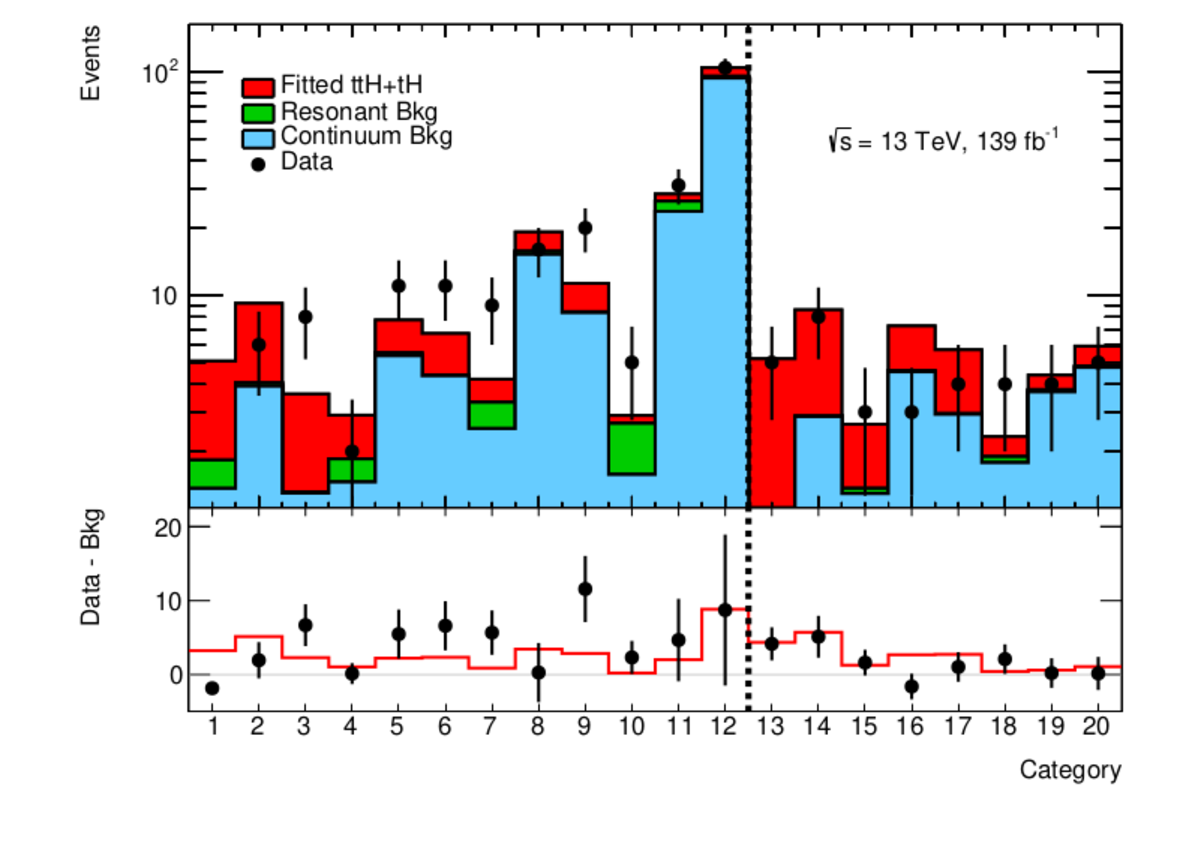
\includegraphics[width=0.6\textwidth]{figures/tthcp_results/yield_S90_obs.pdf}}
    \caption{The signal and background yields calculated in the smallest $m_{\gamma\gamma}$ window containing 90\% of fitted signal in each category. Signal is comprised of $ttH+tHjb+tWH$ and normalized to the Standard Model expectation (a) or the best fit value (b). The data events in this range are overlaid in black points.
\label{fig:yields}}
\end{figure}



\subsection{Observed and Expected $ttH$ Significance}

Expected $ttH$ significance is evaluated using post-fit Asimov data for which the yield of all non-$ttH$ processes is set to the Standard Model value and a Standard Model CP-Even Yukawa Coupling is assumed. The expected $ttH$ significance is 4.4$\sigma$, with an expected signal strength of:
 
\begin{equation}
\mu_{ttH}^exp = 1.00^{+0.32}_{-0.28}
\end{equation}

The observed $ttH$ significance is 5.2$\sigma$ (5.6$\sigma$ if systematics are neglected), corresponding to a signal strength of:

\begin{equation}
\mu_{ttH}^obs = 1.43^{+0.39}_{-0.35}(stat)^{+0.20}_{-0.16}(syst)
\end{equation}
 

This analysis thus marks the first ever single-channel observation of $ttH$ in the diphoton channel with ATLAS: while $ttH$ has been observed in a combination of channels on ATLAS \cite{ttH} and has been observed in the diphoton channel with CMS \cite{ttHCMS}, previous single-channel $ttH$ ATLAS measurements were below the 5.0$\sigma$ threshold needed to constitute a discovery. 
 
\subsection{Upper Limit on $tH$}

Though the small cross-section of the $tH$ process makes it unlikely to be detected in ATLAS Run-2 data alone, it is nonetheless possible to set an upper limit on how large any deviation from the Standard Model must be, given current analysis sensitivity. This is done using the CLs model, a conservative method of setting such limits \cite{CLs}.

Expected $tH$ significance is evaluated using post-fit Asimov data for which the yield of all non-$tH$ or -$ttH$ processes is set to the Standard Model value and a Standard Model CP-Even Yukawa Coupling is assumed. The signal strength terms $\mu_{ttH}$, $\mu_{tWH}$, and $\mu_{tHjb}$ are then allowed to float in the fit. The expected limit is 11.7 $\times$ SM , and the observed limit is 11.6 $\times$ SM (10.5 $\times$ SM neglecting systematics).

\subsection{Limits on $\kappa_{t}$ and $\alpha$}

\subsubsection{2-D Constraint Using Previous Measurements}

A fit is performed using the recent Run-2 Couplings combination result \cite{PhysRevD.101.012002} to constrain the values of $\kappa_{g}$ and $\kappa_{\gamma}$. Because the dataset used for the CP analysis is a subset of the dataset used for the previous Run-2 Couplings combination result, the $ttH$ and $tH$ categories of the analysis are excluded to ensure orthogonal selection and the constraint terms are re-derived for the CP analysis. The constraint terms are:

\begin{equation}
\kappa_{g} = 1.034 \pm 0.067
\kappa_{\gamma} = 0.984 \pm 0.064
\rho(\kappa_{g}, \kappa_{\gamma}) = -0.47
\end{equation}

Where the $\rho$ term governs the correlation between the two \cite{kappaFW}. 

The two-dimensional contour for $\kappa_{g}$ and $\kappa_{\gamma}$ used to perform the constraint is given in Figure \ref{fig:combkgky}. The contours for $\kappa_{t}cos(\alpha)$ and $\kappa_{t}sin(\alpha)$ are shown in Figure \ref{fig:s2:contours}.

\begin{figure}[htbp]
  \centering
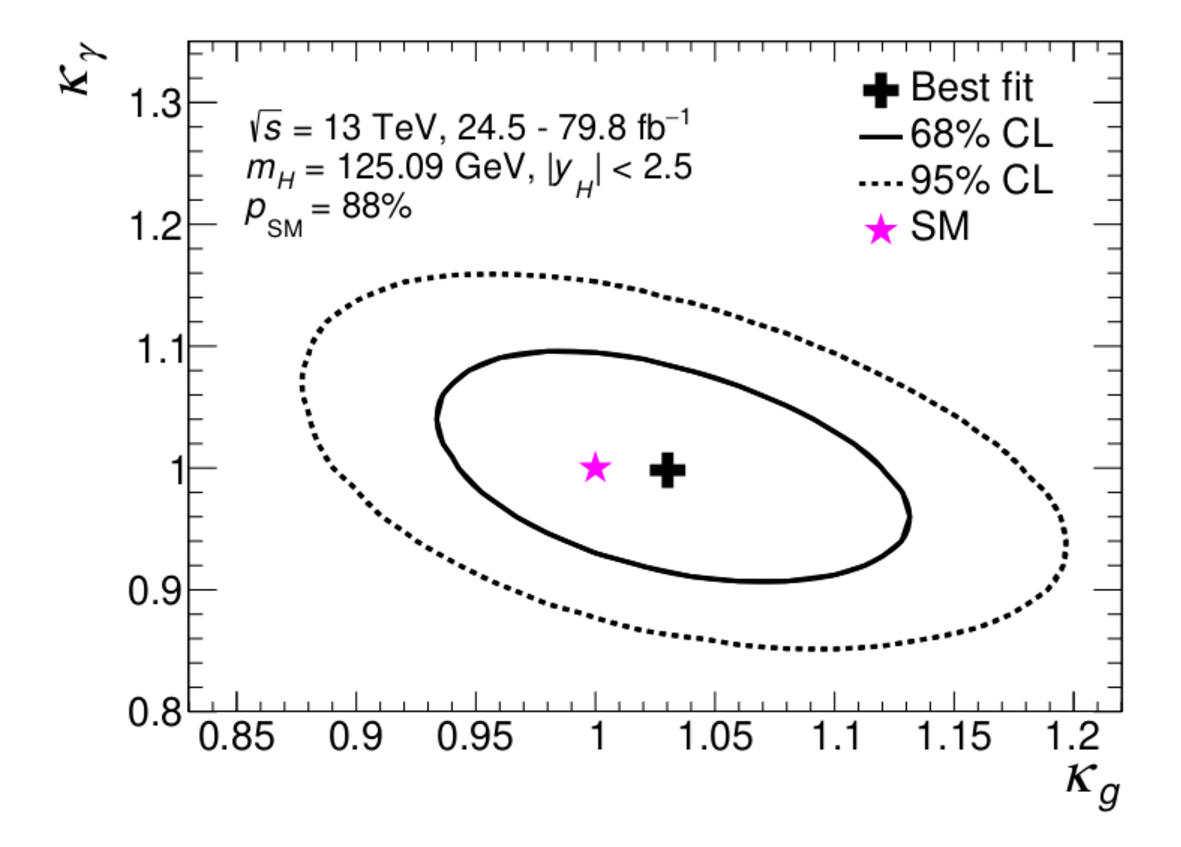
\includegraphics[width=0.5\textwidth]{figures/tthcp_results/combination_kgky.pdf}
\caption{Two-dimensional contour from the ATLAS Higgs coupling combination. The best fit value of $(\kappa_g,\kappa_\gamma)$ is shown with 1 and 2$\sigma$ contours. This is used as a constraint on $ggF$ and $H \rightarrow \gamma\gamma$ in the fit. \label{fig:combkgky}}
\end{figure}

\begin{figure}[htbp]
  \centering
  \subfloat[Expected]{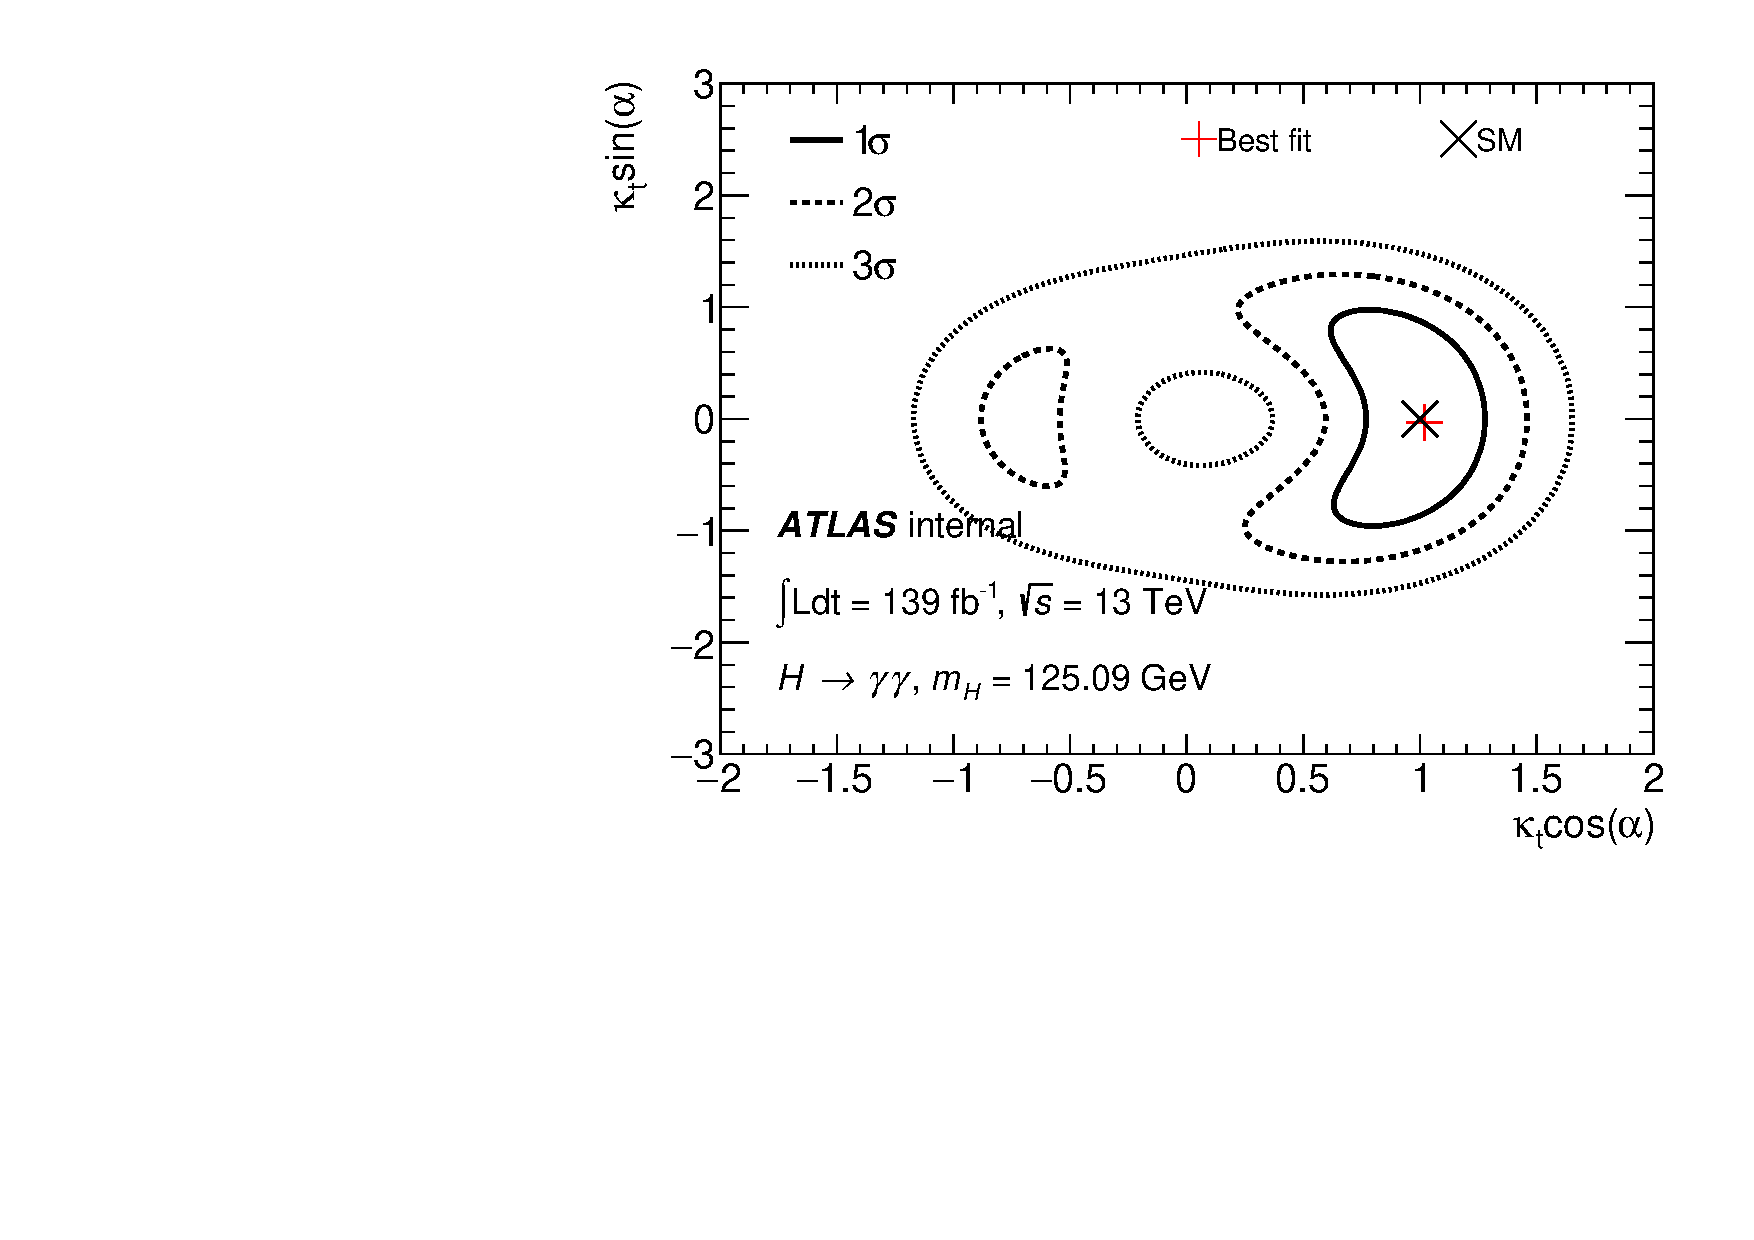
\includegraphics[width=0.4\textwidth]{figures/tthcp_results/kt_even_kt_odd_scale_exp.pdf}}
  \subfloat[Observed]{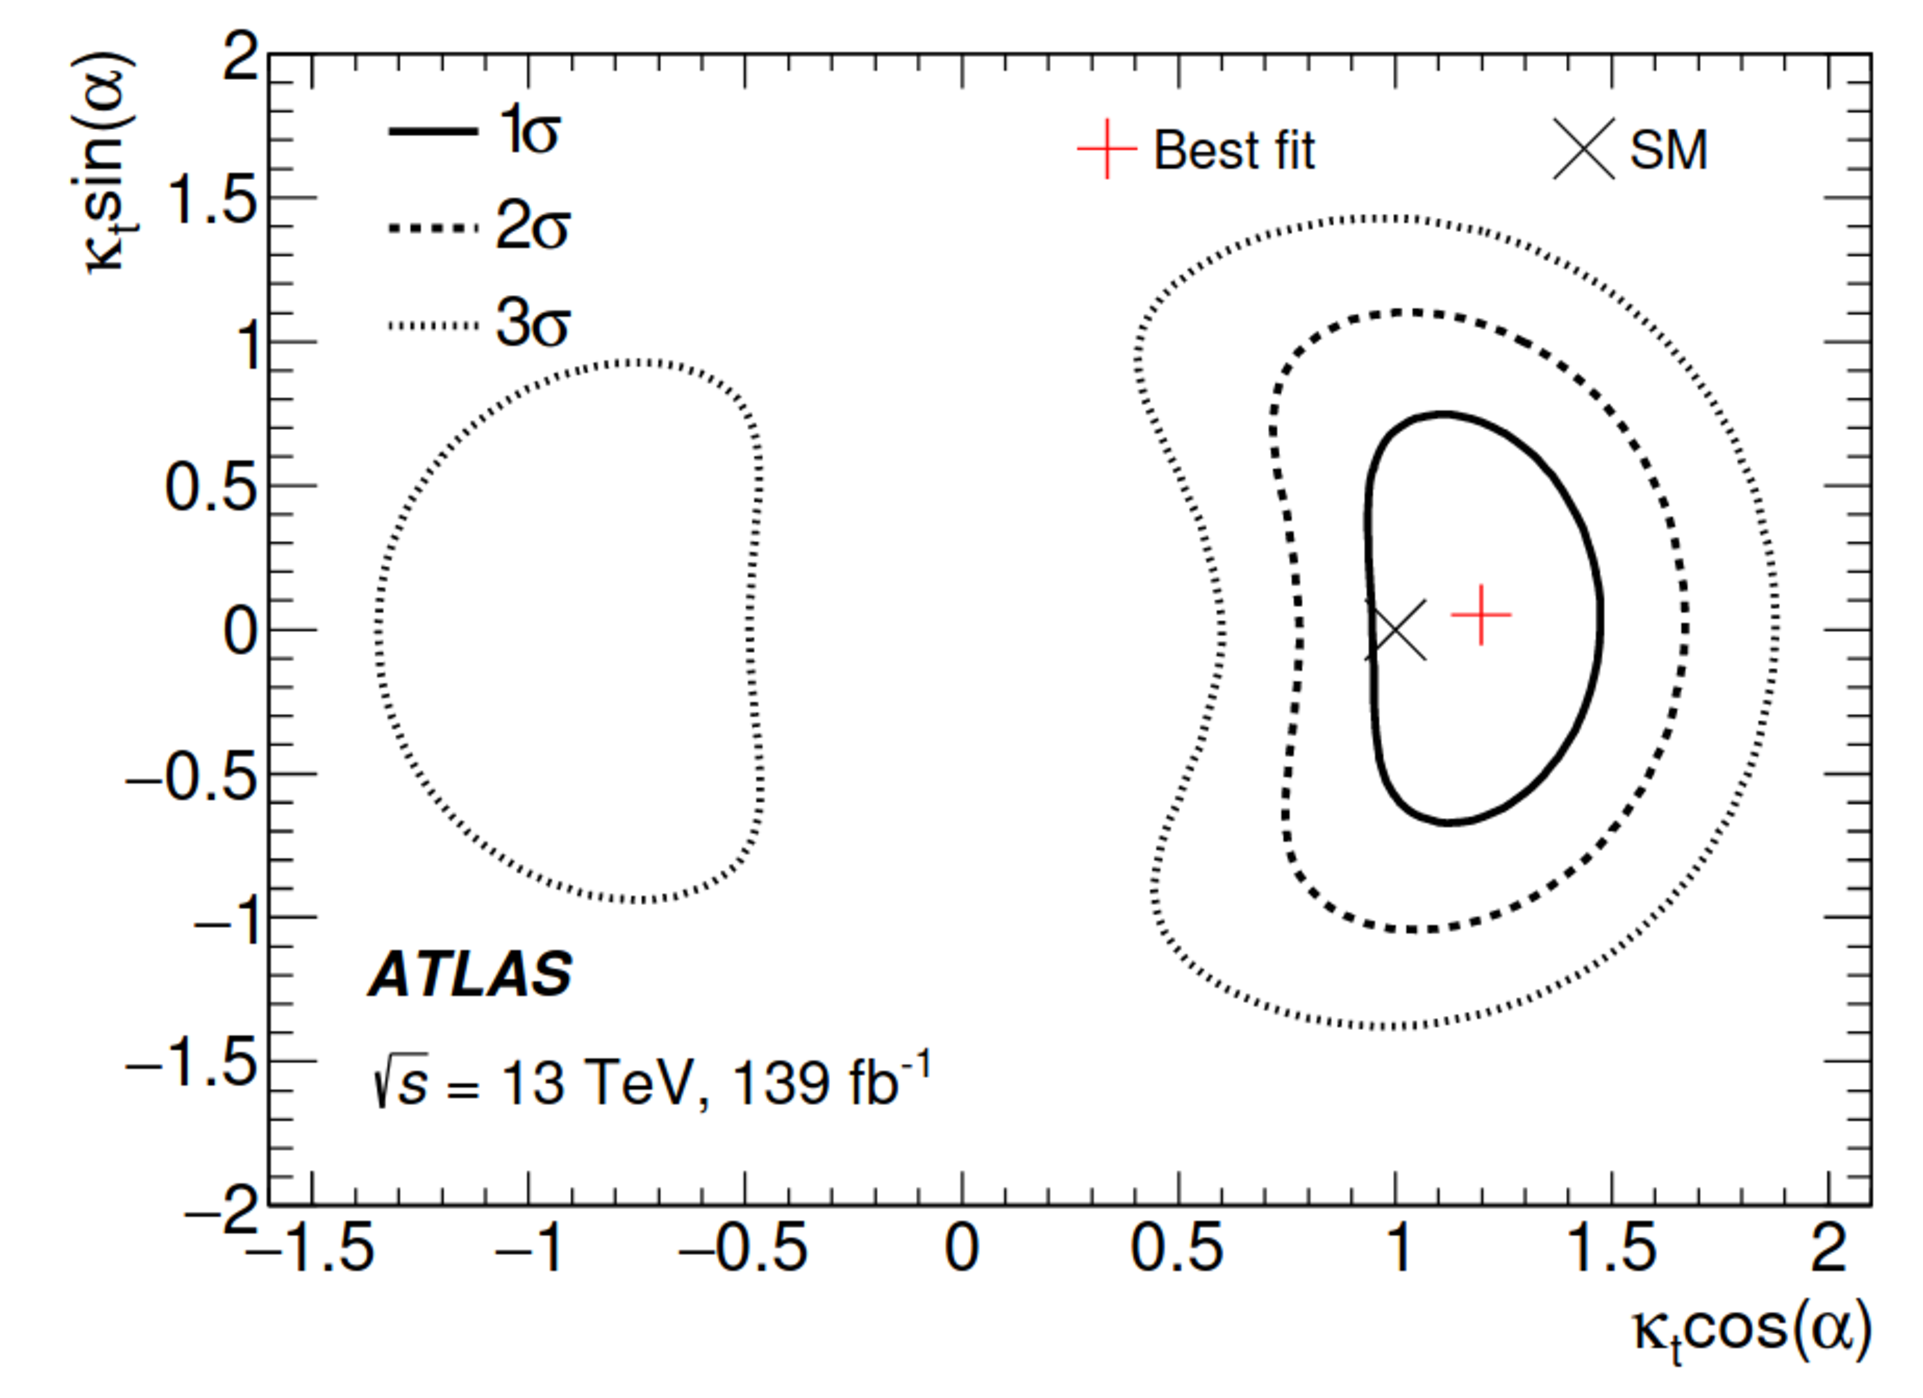
\includegraphics[width=0.4\textwidth]{figures/tthcp_results/kt_even_kt_odd_scale_obs.pdf}}
  \caption{Two-dimensional likelihood contour of $\kappa_t \cos\alpha$ and $\kappa_t \sin\alpha$, with $ggF$ and $H \rightarrow \gamma\gamma$ constrained by the existing Higgs coupling combination result, on (a) post-fit Asimov data and (b) observed data.
  \label{fig:s2:contours}}
\end{figure}

\subsubsection{1-D Constraint Using Previous Measurements}

The 1-D log-likelihood ratio scan performed using the Run-2 couplings combination constraint is shown in Figure \ref{fig:alphascan_expobs_scale}. We find that, assuming the CP-even scenario, the expected exclusion is $\alpha \in$ [$-63^{\circ}$, $63^{\circ}$] at 95\% confidence level. The observed exclusion limit is  $\alpha \in$ [$-40^{\circ}$, $43^{\circ}$] at 95\% confidence level, and the CP odd hypothesis is rejected at the $3.9\sigma$ level. The measured mixing angle is, in degrees, 

\begin{equation}
\alpha = 0.0^{+25.1}_{-21.2}(stat)^{+2.8}_{-1.7}(syst)
\end{equation}

\begin{figure}[htbp]
  \centering
  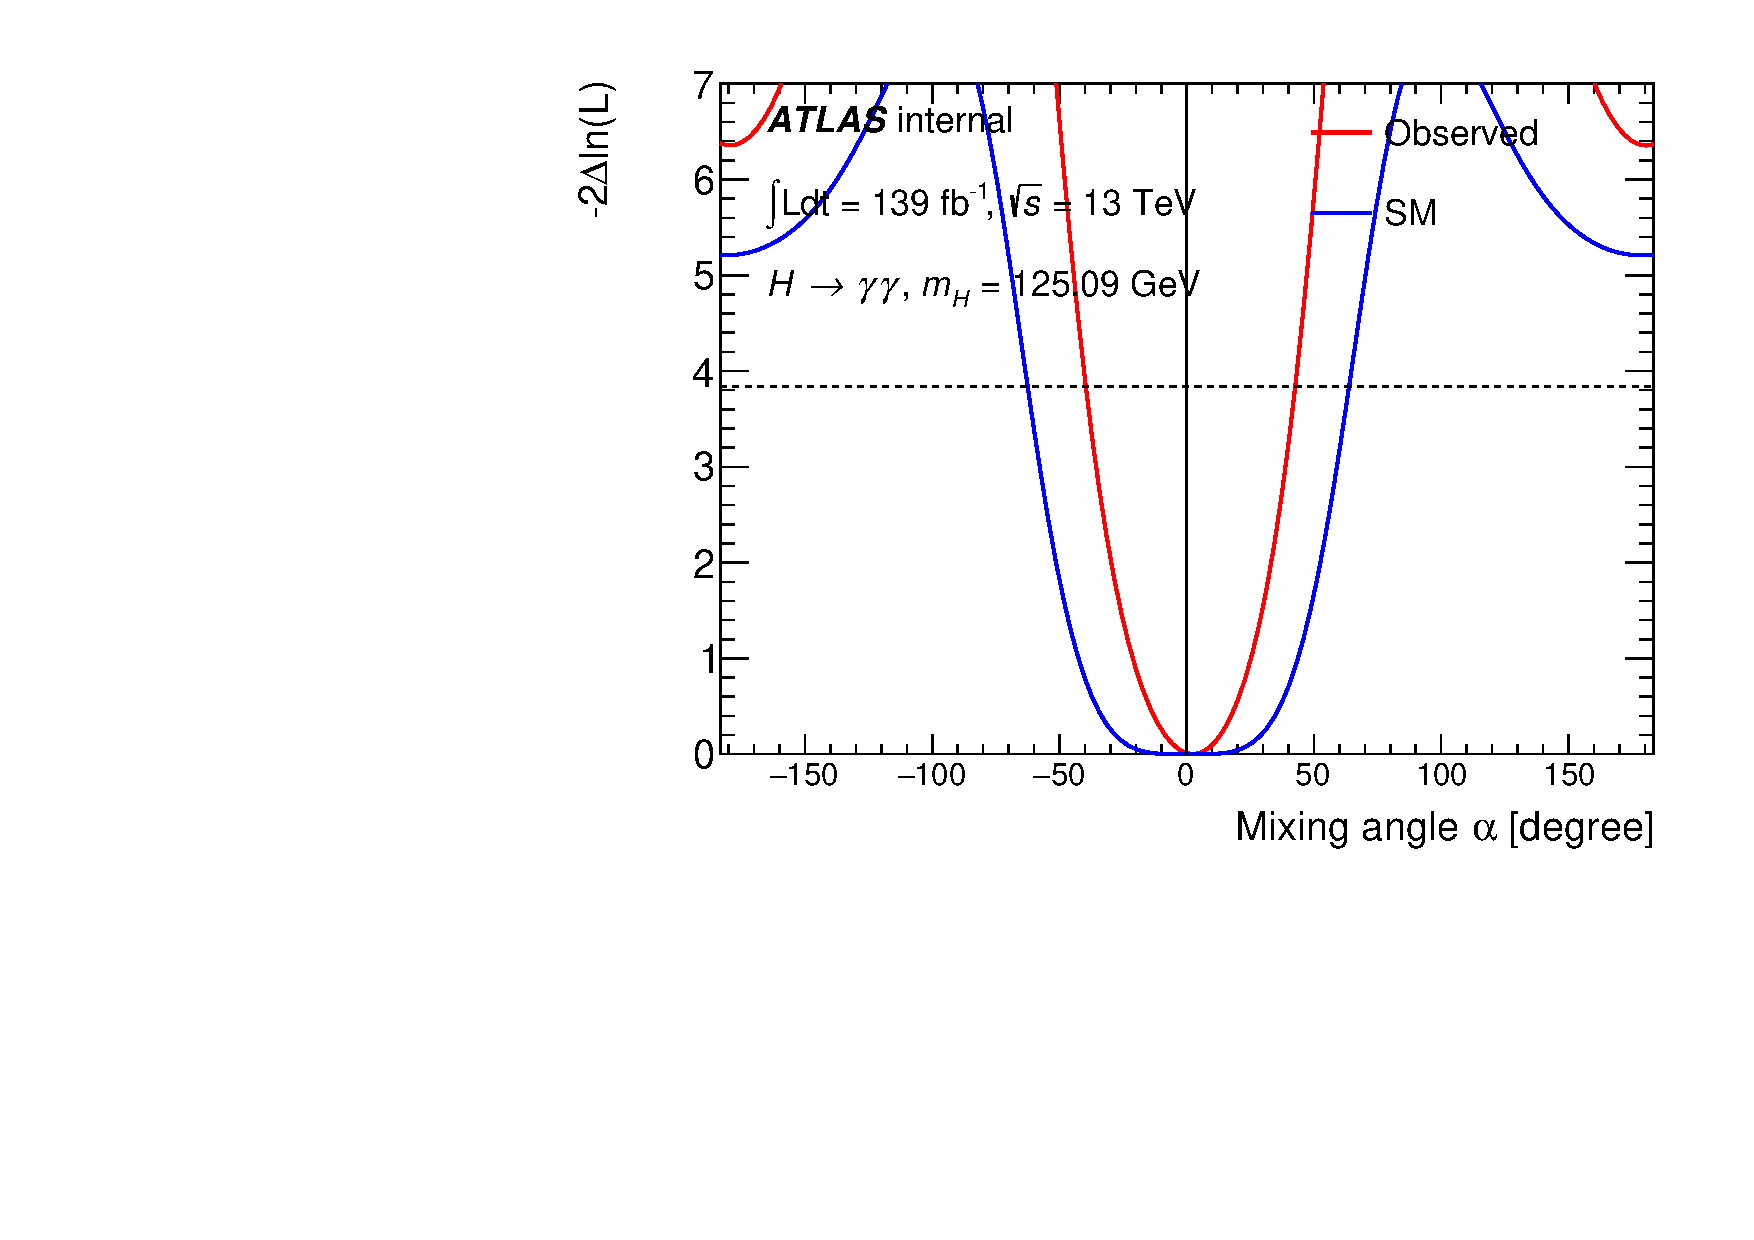
\includegraphics[width=0.4\textwidth]{figures/tthcp_results/nllscan_alpha_expobs_scale.pdf}
  \caption{One-dimensional likelihood scan over possible values of the CP-mixing angle $\alpha$ on post-fit Asimov data (blue) and observed data (red). $ggF$ and $H \rightarrow \gamma\gamma$ are constrained by the previous Higgs coupling combination result.
  \label{fig:alphascan_expobs_scale}}
\end{figure}

A test is also done to check whether allowing the Higgs-W coupling $\kappa_{V}$ to float in this manner rather than fixing it to the Standard Model value affects the results; effects were found to be negligible.

\subsubsection{2-D Constraint Using $\kappa_{t}$ Parameterization}

Parameterizing $\kappa_{g}$ and $\kappa_{\gamma}$ in terms of $\kappa_{t}$ is model-dependent, that is, it assumes that no other unknown physics phenomena enter the top-quark loops governing the $ggF$ and $H \rightarrow \gamma \gamma$ processes. The observed and expected contours are shown in Figure \ref{fig:s3:contours}: allowing $H \rightarrow \gamma \gamma$ to constrain the effects of $\alpha$ substantially increases the sensitivity of the analysis, in particular constraining negative values of $\kappa_{t} cos(\alpha)$.

In the observed results, the negative branch of $\kappa_{t}cos(\alpha)$ is rejected at $> 3\sigma$. Higher values of $\kappa_{t}$ are allowed in this interpretation since the existing constraints on $ggF$ and $H \rightarrow \gamma \gamma$ are not applied.

At values near $\kappa_{t} = 4.7$, the $H \rightarrow \gamma \gamma$ branching ratio drops to zero: the presence of a $H \rightarrow \gamma \gamma$ signal in observed data thus means this region is excluded, hence the large hole in the two-dimensional contour.

\begin{figure}[htbp]
  \centering
  \subfloat[Expected]{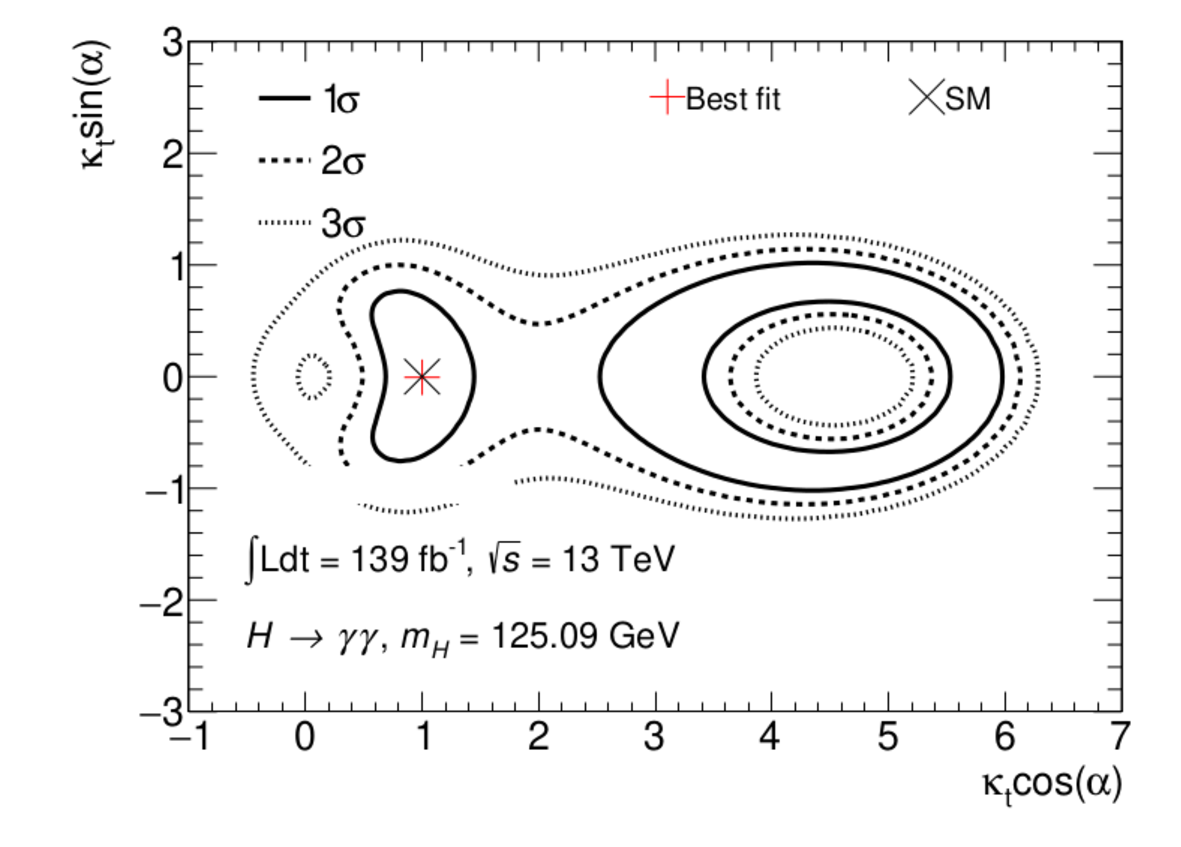
\includegraphics[width=0.4\textwidth]{figures/tthcp_results/kt_even_kt_odd_resolve_exp.pdf}}
  \subfloat[Observed]{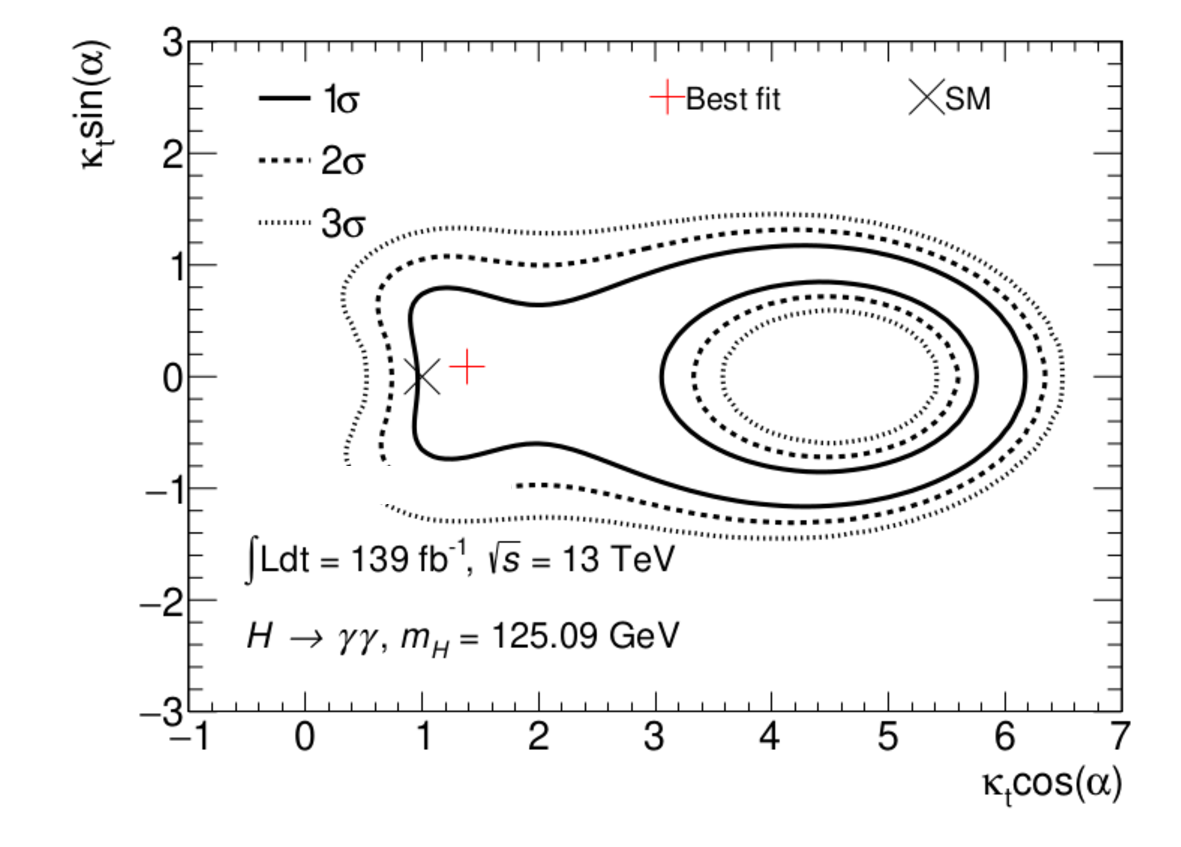
\includegraphics[width=0.4\textwidth]{figures/tthcp_results/kt_even_kt_odd_resolve_obs.pdf}}
  \caption{Two-dimensional likelihood contour of $\kappa_t \cos\alpha$ and $\kappa_t \sin\alpha$, with $ggF$ and $H \rightarrow \gamma\gamma$ parameterized as function of $\kappa_t$ and $\alpha$, on (a) post-fit Asimov data and (b) observed data.
  \label{fig:s3:contours}}
\end{figure}

\subsubsection{1-D Constraint Using $\kappa_{t}$ Parameterization}

The 1-D log-likelihood ratio scan performed using the Run-2 couplings combination constraint is shown in Figure \ref{fig:alphascan_expobs_resolve}. We find that, assuming the CP-even scenario, the expected exclusion is $\alpha \in$ [$-55^{\circ}$, $56^{\circ}$] at 95\% confidence level. The observed exclusion limit is  $\alpha \in$ [$-41^{\circ}$, $43^{\circ}$] at 95\% confidence level, and the CP odd hypothesis is rejected at the $4.0\sigma$ level. The measured mixing angle is, in degrees, 

\begin{equation}
\alpha = 0.1^{+26.6}_{-23.2}(stat)^{+7.4}_{-5.2}(syst)
\end{equation}

\begin{figure}[htbp]
  \centering
  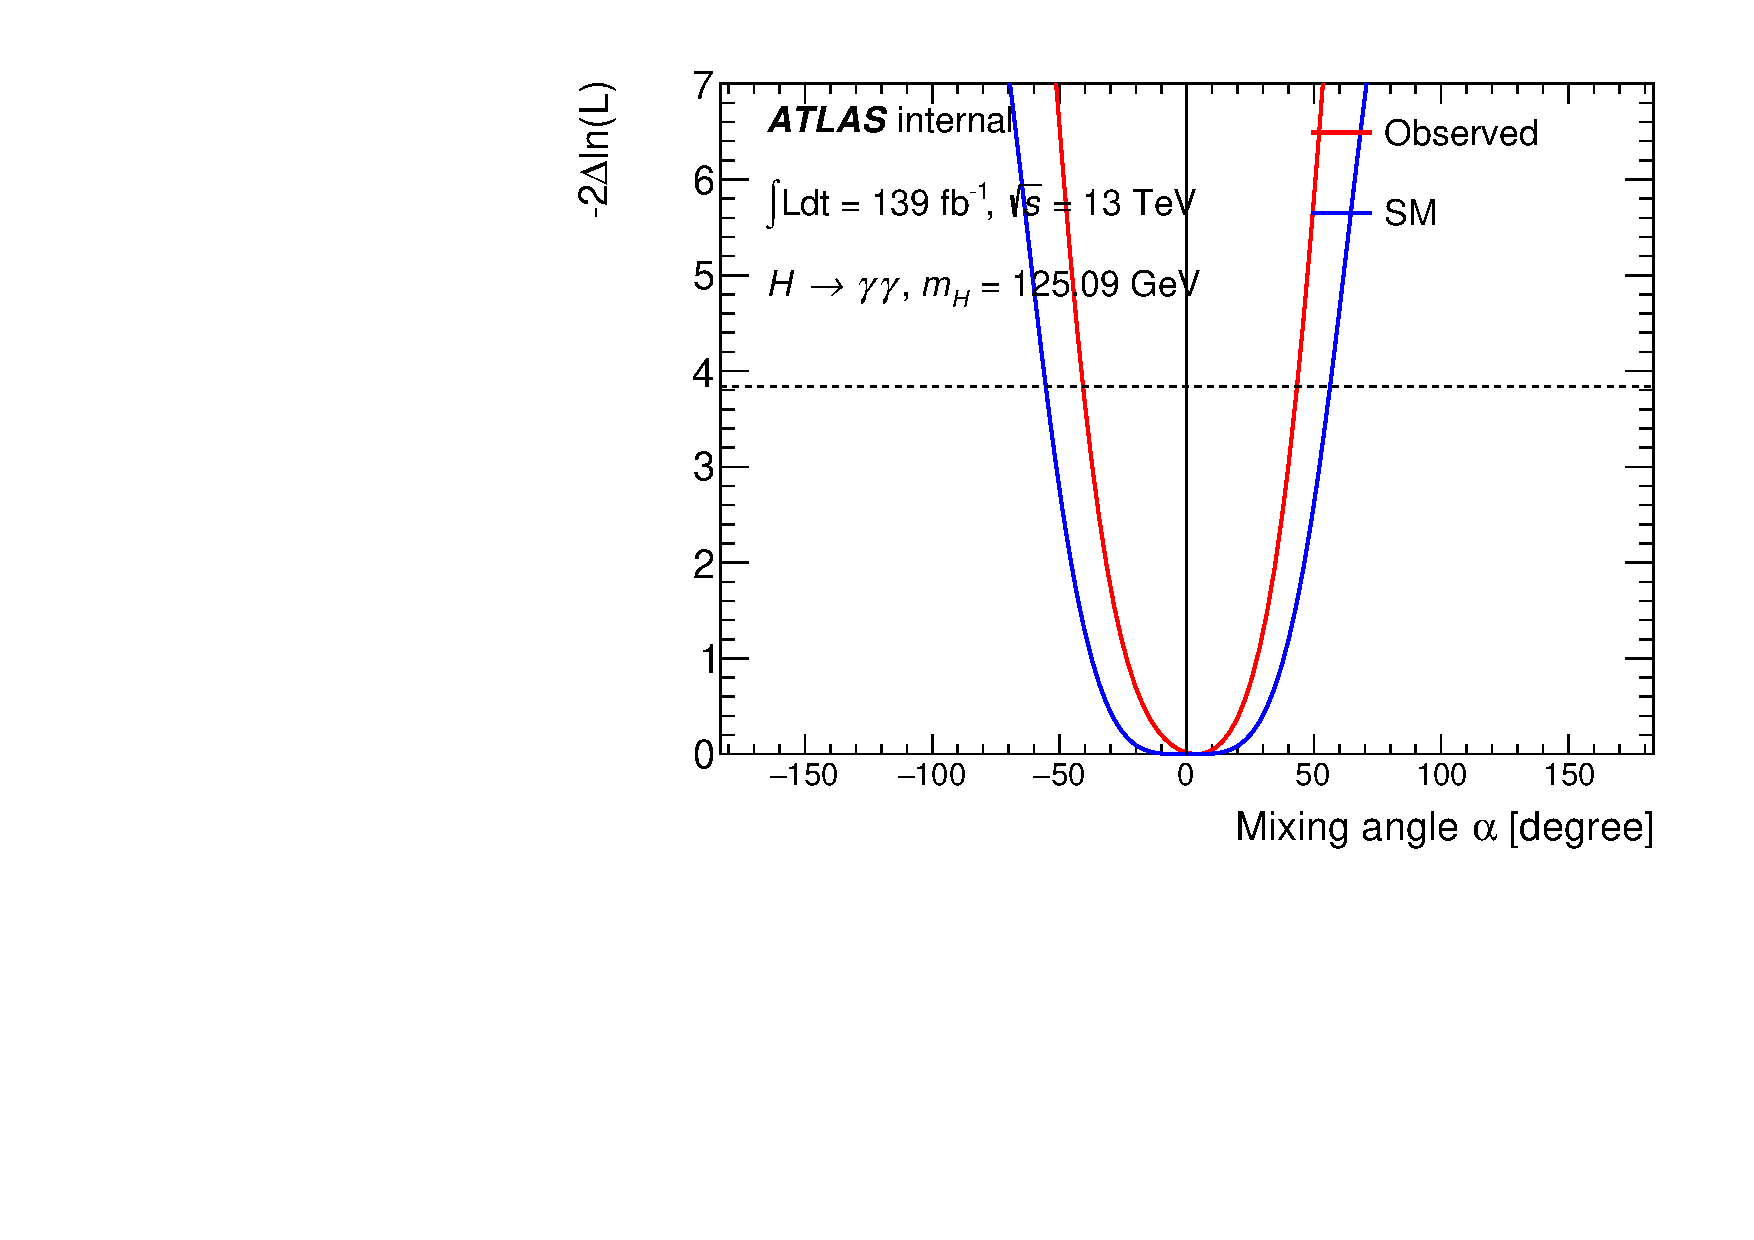
\includegraphics[width=0.4\textwidth]{figures/tthcp_results/nllscan_alpha_expobs_resolve.pdf}
  \caption{One-dimensional likelihood scan over possible values of the CP mixing angle $\alpha$ on post-fit Asimov data (blue) and observed data (red).  $ggF$ and $H \rightarrow \gamma\gamma$ are parameterized as functions of $\kappa_t$ and $\alpha$.
  \label{fig:alphascan_expobs_resolve}}
\end{figure}
